\documentclass[12pt,a4paper]{report}

% ===== BASIC PACKAGES =====
\usepackage[utf8]{inputenc}
\usepackage[T1]{fontenc}
\usepackage{fontspec}
\IfFontExistsTF{Times New Roman}{\setmainfont{Times New Roman}}{\setmainfont{Liberation Serif}}

% ===== VIETNAMESE CHAPTER/FIGURE/TABLE LABELS (manual, no polyglossia needed) =====
\renewcommand{\contentsname}{MỤC LỤC}
\renewcommand{\listfigurename}{DANH MỤC HÌNH VẼ}
\renewcommand{\listtablename}{DANH MỤC BẢNG}
\renewcommand{\figurename}{Hình}
\renewcommand{\tablename}{Bảng}
\renewcommand{\chaptername}{Chương}
\renewcommand{\bibname}{TÀI LIỆU THAM KHẢO}
\usepackage{titlesec}
\titleformat{\chapter}[display]
  {\normalfont\huge\bfseries}{\chaptertitlename\ \thechapter}{20pt}{\Huge}
\titlespacing*{\chapter}{0pt}{0pt}{30pt}

% ===== PAGE LAYOUT =====
\usepackage[a4paper,top=3cm,bottom=3cm,left=3.5cm,right=2cm]{geometry}
\usepackage{setspace}
\onehalfspacing

% ===== GRAPHICS AND TABLES =====
\usepackage{graphicx}
\usepackage[export]{adjustbox}
\usepackage{booktabs}
\usepackage{multirow}
\usepackage{longtable}
\usepackage{array}
\usepackage{tabularx}
\usepackage{caption}
\usepackage{float}
\usepackage{xcolor}
\usepackage{tikz}
\usetikzlibrary{shapes.callouts, positioning, arrows.meta, fit, backgrounds, shapes.arrows}

\newcolumntype{L}[1]{>{\raggedright\arraybackslash}p{#1}}
\newcolumntype{C}[1]{>{\centering\arraybackslash}p{#1}}
\newcolumntype{R}[1]{>{\raggedleft\arraybackslash}p{#1}}

% ===== MATHEMATICS =====
\usepackage{amsmath,amssymb}

% ===== GANTT CHART =====
\usepackage{pgfgantt}

% ===== HYPERLINKS =====
\usepackage[hidelinks]{hyperref}
\usepackage{url}

% ===== HEADER AND FOOTER =====
\usepackage{fancyhdr}
\setlength{\headheight}{15.1pt}
\pagestyle{fancy}
\fancyhf{}
\fancyhead[R]{\thepage}
\fancyhead[L]{\nouppercase{\leftmark}}
\renewcommand{\headrulewidth}{0.5pt}

\fancypagestyle{plain}{%
    \fancyhf{}
    \fancyfoot[C]{\thepage}
    \renewcommand{\headrulewidth}{0pt}
}

\definecolor{hustblue}{RGB}{0,60,113}
\definecolor{goodgreen}{RGB}{30,120,60}
\definecolor{warnorange}{RGB}{200,90,20}
\definecolor{badred}{RGB}{170,30,30}
\definecolor{hustgray}{RGB}{90,95,107}

% ===== BEGIN DOCUMENT =====
\begin{document}

% ===== TITLE PAGE =====
\begin{titlepage}
\thispagestyle{empty}
\begin{center}
    \normalsize{\textbf{ĐẠI HỌC BÁCH KHOA HÀ NỘI}}\\
    \normalsize{\textbf{TRƯỜNG CÔNG NGHỆ THÔNG TIN VÀ TRUYỀN THÔNG}}\\[0.3cm]

    \vspace{0.2cm}
    
\includegraphics[width=2.5cm]{figures/hust_logo.png}
    \vspace{0.2cm}

    \Large{\textbf{BÁO CÁO CUỐI KỲ}}\\[0.2cm]
    \Large{\textbf{HỌC PHẦN IT5427 — TÍCH HỢP VÀ XỬ LÝ DỮ LIỆU LỚN}}\\[1cm]

    \LARGE{\textbf{Hệ thống tích hợp và xử lý dữ liệu khí tượng}}\\[0.15cm]
    \LARGE{\textbf{đa nguồn phục vụ phát hiện dị thường khí hậu}}\\[0.15cm]
    \LARGE{\textbf{và hỗ trợ ra quyết định đa ngành}}\\[0.3cm]

    \large{\textbf{Khu vực Đông Nam Á}}\\[1.5cm]

    \begin{flushleft}
    \small
    \hspace{1.5cm}\begin{tabular}{@{}ll@{}}
    \textbf{Nhóm:} & 16 \\[0.15cm]
    \textbf{Thành viên:} & Ngô Văn Quang -- 20251243M \\
     & Nguyễn Cao Lương -- 20251244M \\
     & Trương Tuấn Nghĩa -- 20251196M \\[0.15cm]
    \textbf{Học phần:} & IT5427 -- Tích hợp và xử lý dữ liệu lớn \\[0.15cm]
    \textbf{Giảng viên hướng dẫn:} & TS. Vũ Tuyết Trinh \\[0.15cm]
    \textbf{Đơn vị:} & Trường Công nghệ Thông tin và Truyền thông \\[0.4cm]
    \end{tabular}
    \end{flushleft}

    \vfill

    \large{\textbf{Hà Nội, Tháng 11/2026}}

\end{center}
\end{titlepage}

% ===== FRONT MATTER =====
\pagenumbering{roman}
\setcounter{page}{1}

\tableofcontents
\clearpage

\listoffigures
\addcontentsline{toc}{chapter}{DANH MỤC HÌNH VẼ}
\clearpage

\listoftables
\addcontentsline{toc}{chapter}{DANH MỤC BẢNG}
\clearpage

\chapter*{DANH MỤC TỪ VIẾT TẮT}
\addcontentsline{toc}{chapter}{DANH MỤC TỪ VIẾT TẮT}

\begin{tabular}{@{}ll@{}}
\toprule
\textbf{Từ viết tắt} & \textbf{Giải nghĩa} \\
\midrule
API & Application Programming Interface \\
ASMC & ASEAN Specialised Meteorological Centre \\
CDS & Climate Data Store (Copernicus) \\
ĐNA & Đông Nam Á \\
ER & Entity Resolution \\
ERA5 & ECMWF Reanalysis v5 \\
ETL & Extract, Transform, Load \\
GAV & Global-as-View \\
GHCN & Global Historical Climatology Network \\
ISD & Integrated Surface Database (NOAA) \\
LAV & Local-as-View \\
LSH & Locality-Sensitive Hashing \\
PINN & Physics-Informed Neural Network \\
QC & Quality Control \\
SEA & Southeast Asia \\
TGD & Tuple Generating Dependency \\
TV & Thành viên \\
UAV & Unmanned Aerial Vehicle \\
\bottomrule
\end{tabular}

\clearpage
\pagenumbering{arabic}
\setcounter{page}{1}

% ==========================================================
\chapter{Giới thiệu}
% ==========================================================

\section{Bối cảnh và động lực}

Dữ liệu khí tượng minh hoạ rõ bài toán tích hợp dữ liệu lớn: khối lượng lớn (ERA5 sinh hàng chục
terabyte mỗi năm) đi cùng sự đa dạng cực đoan về nguồn gốc và định dạng, từ lưới liên tục của mô hình số
trị tới chuỗi thời gian rời rạc của hàng chục nghìn trạm mặt đất. Đông Nam Á là bối cảnh phù hợp: khí hậu
nhiệt đới gió mùa chịu nhiều hiện tượng cực đoan (mưa lớn, bão, hạn), trong khi mật độ trạm quan trắc
rất không đồng đều giữa các nước, buộc bài toán tích hợp phải được giải quyết thật sự.

Đề tài khớp trực tiếp với hai trụ cột của học phần IT5427: \textbf{Schema Alignment} (ánh xạ lược đồ
giữa các nguồn khác cấu trúc) và \textbf{Record Linkage / Entity Resolution} (liên kết bản ghi do các
nguồn độc lập đo cùng một hiện tượng), cùng các kỹ thuật xử lý phân tán bằng Apache Spark.

\section{Phát biểu bài toán}

Bài toán cốt lõi: \emph{hợp nhất năm nguồn khí tượng không tương thích (lưới ERA5; chuỗi trạm NOAA
GHCN-Daily và NOAA ISD; truy vấn điểm NASA POWER và Open-Meteo) thành một kho thống nhất, đáng tin cậy,
dùng trực tiếp được cho phân tích.}

Bài toán bộc lộ đủ 7/7 mức dị biệt của học phần: (1) \emph{nền tảng}: REST API JSON, CSV trên AWS S3,
Zarr/CDS API; (2) \emph{cú pháp}: NetCDF/GRIB2, CSV, JSON lồng; (3) \emph{lược đồ}: GHCN dạng ``long'',
bốn nguồn còn lại dạng ``wide''; (4) \emph{ngữ nghĩa}: áp suất bề mặt khác áp suất mực nước biển, bốn
định nghĩa ``nhiệt độ ngày''; (5) \emph{định danh}: cùng một trạm mang hai mã GHCN/ISD (Mục~6.2); (6)
\emph{thời gian}: giờ địa phương so với UTC, tần suất ngày so với giờ; (7) \emph{chất lượng}: mỗi nguồn
một cơ chế QC, cần quy tắc Survivorship (Mục~3.3).

\section{Mục tiêu đề tài}

Đề tài có năm mục tiêu:

\begin{enumerate}
    \item Xây dựng \textbf{kho dữ liệu khí tượng chuẩn hoá} (Mediated Schema) tích hợp đủ năm nguồn, dùng
    lại được cho nhiều bài toán phân tích.
    \item Áp dụng có kiểm chứng \textbf{GAV schema mapping} và \textbf{Survivorship-based Data Fusion} trên
    dữ liệu thật.
    \item Xây dựng pipeline \textbf{Apache Spark} hoàn chỉnh (batch và Structured Streaming), đạt tiêu chí
    5V bằng số liệu định lượng.
    \item Triển khai \textbf{phát hiện dị thường khí hậu} theo khu vực và thời điểm, đối chứng với sự kiện
    thật (Mục~6.8--6.10). Hai ứng dụng hỗ trợ nông nghiệp/năng lượng và khung giờ bay UAV chưa cài đặt
    (Chương~9).
    \item Xây dựng \textbf{dashboard trực quan hoá} theo không gian/thời gian (Direction 1 của đề cương).
\end{enumerate}

\section{Mục tiêu đo được}

Mỗi mục tiêu được gắn với một chỉ số đo (Bảng~\ref{tab:measurable-goals}), ghi rõ ngưỡng đặt trước
khi có kết quả hay chỉ biết sau khi đo. Đối chiếu với kết quả thật nằm ở Bảng~\ref{tab:goals-vs-results}
(Chương~9).

\begin{table}[H]
\centering
\caption{Mục tiêu đo được và ngưỡng đặt ra}
\label{tab:measurable-goals}
\begin{tabular}{@{}L{0.8cm}L{4.4cm}L{4.2cm}L{3.4cm}@{}}
\toprule
\textbf{Mã} & \textbf{Mục tiêu (Mục 1.3)} & \textbf{Chỉ số đo} & \textbf{Ngưỡng / thời điểm đặt} \\
\midrule
M1 & Kho dữ liệu chuẩn hoá đủ 5 nguồn, đúng phạm vi đề cương & Số nguồn tích hợp, đúng phạm vi thời gian/không gian & Đủ 5/5, đúng phạm vi -- đặt trước (Mục~1.4) \\
M2 & GAV schema mapping + Entity Resolution/Survivorship có kiểm chứng định lượng & Referential integrity (GAV); precision/recall Entity Resolution GHCN--ISD; tỷ lệ xung đột Survivorship theo biến & Phải kiểm chứng bằng số liệu thật, không chỉ minh hoạ -- đặt trước (Mục~1.3); tỷ lệ \% chỉ biết sau khi đo \\
M3 & Pipeline Spark tối ưu hoá có đo trước/sau, đạt 5V bằng số liệu & Tăng tốc khi \texttt{cache()} một truy vấn đại diện & $\geq 30\,\%$ -- đặt trước (Mục~1.4, cùng thời điểm với M1, M2) \\
M4 & Phát hiện dị thường khí hậu đối chứng được với sự kiện thật & Số sự kiện khí hậu đã biết được phát hiện đúng chiều & 3 sự kiện đối chứng chọn trước (nắng nóng 2024, bão Yagi, hạn Mekong); kết quả từng sự kiện chỉ biết sau khi đo \\
M5 & Dashboard hiển thị đúng kết quả tích hợp, kiểm chứng qua trình duyệt thật & Số thành phần hoạt động đúng trên dữ liệu thật, không lỗi runtime & Đặt trước (đề cương học phần, Direction 1) \\
\bottomrule
\end{tabular}
\end{table}

Mô hình PINN trường gió (hạng mục tuỳ chọn, Mục~5.3) được đánh giá bằng RMSE so với hồi quy thuần
trên tập kiểm tra giữ lại, không theo ngưỡng đạt/không đạt.

\section{Phạm vi và giới hạn}

Phạm vi không gian là Đông Nam Á lục địa và hải đảo (vĩ độ $-11^\circ$ đến $23^\circ$, kinh độ
$92^\circ$ đến $141^\circ$); cửa sổ kết quả là 2020--2024, giai đoạn cả năm nguồn bắt buộc (ERA5, GHCN-Daily,
ISD, NASA POWER, Open-Meteo) cùng có dữ liệu. Chuỗi GHCN dài hơn chỉ dùng làm khí hậu nền 1991--2020 và
tính xu hướng 30 năm. Himawari và CHIRPS là nguồn tuỳ chọn, ngoài phạm vi sáu tuần của nhóm ba người.

% ==========================================================
\chapter{Tổng quan tài liệu và cơ sở lý thuyết}
% ==========================================================

Chương này tóm tắt cơ sở lý thuyết theo các kỹ thuật được áp dụng ở Chương~3.

\section{Đối sánh lược đồ và ngôn ngữ ánh xạ (Schema Matching \& Mapping)}

Rahm và Bernstein~\cite{rahm2001survey} hệ thống hoá đối sánh lược đồ tự động theo cấp độ
(schema-level, instance-level) và theo kỹ thuật (ngôn ngữ, ràng buộc); đây là cơ sở chọn chiến lược ánh
xạ trường giữa năm nguồn (Mục~3.2).

Ba ngôn ngữ ánh xạ GAV, LAV và GLAV bắt nguồn từ các công trình về trả lời truy vấn qua view của
Ullman~\cite{ullman1997logical}, độ phức tạp \emph{certain answers} của Abiteboul và
Duschka~\cite{abiteboul1998complexity}, và được tổng hợp bởi Levy~\cite{levy2001survey} và
Lenzerini~\cite{lenzerini2002theoretical}. GAV định nghĩa mỗi quan hệ toàn cục $G$ bằng một truy vấn trên
các nguồn, $G \supseteq Q(\text{sources})$, nên trả lời truy vấn chỉ cần khai triển $Q$. Đề tài chọn GAV vì
số nguồn cố định và mỗi nguồn ánh xạ bằng một view duy nhất, không cần suy luận ngược như LAV.

Khi số nguồn lớn và thay đổi liên tục, Halevy và cộng sự đề xuất \emph{Dataspace}~\cite{halevy2006dataspace},
Das Sarma và cộng sự đề xuất \emph{pay-as-you-go}~\cite{dassarma2008payasyougo}; Cafarella và cộng
sự~\cite{cafarella2008webtables} và Talukdar và cộng sự~\cite{talukdar2008learning} tích hợp không cần
mediated schema tường minh. Với năm nguồn cố định, đề tài không cần độ linh hoạt này.

\section{Liên kết bản ghi và giải quyết thực thể (Record Linkage \& Entity Resolution)}

Mô hình xác suất của Fellegi và Sunter~\cite{fellegi1969theory} hình thức hoá ba kết luận
\emph{match}, \emph{non-match} và \emph{possible-match} cho một cặp bản ghi; Mục~6.2 áp dụng nó để quyết định hai mã trạm
GHCN/ISD có cùng một trạm vật lý. Survivorship (Bảng~\ref{tab:survivorship}) là bài toán khác: hợp giải giá
trị (\emph{data fusion}) sau khi đã xác định cùng thực thể.

Entity Resolution thường gồm Prepare, Block, Match, Cluster, được Köpcke và cộng
sự~\cite{kopcke2010evaluation} đánh giá có hệ thống. Với 26 trạm ISD $\times$ 41 trạm GHCN $=$ 1.066 cặp,
nhóm so toàn bộ cặp, vì Blocking/LSH~\cite{gionis1999similarity} chỉ có lợi khi số bản ghi lớn hơn nhiều bậc;
ràng buộc 1--1 cũng khiến Clustering~\cite{bansal2004correlation,hassanzadeh2009framework} không cần thiết.

Các hướng học sâu gồm DeepER~\cite{ebraheem2018deeper} và DeepMatcher~\cite{mudgal2018deep}; khi nhãn khan
hiếm, Kasai và cộng sự~\cite{kasai2019lowresource} kết hợp transfer learning và active learning. Burdick và
cộng sự~\cite{burdick2017expressive} hình thức hoá \emph{entity-linking framework} tổng quát; Gruenheid và
cộng sự~\cite{gruenheid2014incremental} đề xuất liên kết gia tăng cho dữ liệu cập nhật liên tục.

\section{Học máy ràng buộc vật lý (Physics-Informed Machine Learning)}

PINN của Raissi và cộng sự~\cite{raissi2019physics} nhúng phương trình vật lý chi phối (ở đây
Clausius--Clapeyron và phương trình liên tục) vào hàm mất mát của mạng nơ-ron thay vì chỉ học từ dữ liệu.
Đề tài dùng PINN như hạng mục tuỳ chọn nâng cao, có phương án lùi về hồi quy thông thường (Mục~5.3).

\section{Dữ liệu tái phân tích khí quyển ERA5}

ERA5~\cite{hersbach2020era5} là tái phân tích thế hệ thứ năm của ECMWF, đồng hoá quan trắc vệ tinh và
mặt đất qua mô hình số trị, độ phân giải $0{,}25°$ theo giờ từ 1940. Bản chất lưới của ERA5, đối lập với
điểm trạm rời rạc, là nguồn gốc của dị biệt cấu trúc trung tâm mà đề tài giải quyết.

\section{Khoảng trống dẫn tới đề tài}

Các công trình trên giải quyết \emph{riêng rẽ} từng bài toán con (schema matching, record linkage,
physics-informed learning) trên dữ liệu bảng quan hệ thông thường. Chưa có công trình nào trong danh mục
tham khảo áp dụng \emph{đồng thời} GAV, Entity Resolution kèm Survivorship và lấp khoảng trống có ràng
buộc vật lý trên dữ liệu khí tượng đa nguồn Đông Nam Á, nơi dị biệt lưới--điểm rõ nét. Đề tài không đề
xuất kỹ thuật mới mà kiểm chứng và tích hợp có hệ thống các kỹ thuật đã có, trên dữ liệu thật.

% ==========================================================
\chapter{Phương pháp luận và kiến trúc hệ thống}
% ==========================================================

\section{Kiến trúc tổng thể}

Hình~\ref{fig:pipeline} trình bày pipeline đã triển khai: năm nguồn qua Ingestion và kiểm soát chất
lượng 4 tầng, hội tụ về Mediated Schema và kho Parquet; từ kho rẽ nhánh xử lý theo lô (Entity Resolution,
dị thường, xu hướng, trôi cảm biến, PINN) và nhánh luồng giả lập qua Kafka, cùng phục vụ Dashboard. Mọi
con số trong hình là số liệu cuối cùng, chạy trên kho đầy đủ sau khi ERA5 tải đủ 540/540 file.

\begin{figure}[H]
\centering
\resizebox{\textwidth}{!}{%
\begin{tikzpicture}[
  chev/.style={signal, signal to=east, signal pointer angle=125, draw=white, line width=1.2pt, text=white, font=\bfseries\footnotesize, align=center, minimum height=1.0cm, minimum width=3.3cm, inner sep=1pt},
  stagebox/.style={rectangle, rounded corners=3pt, line width=1pt, minimum width=2.85cm, minimum height=5.4cm},
  boxtxt/.style={anchor=north, font=\fontsize{10}{11.2}\selectfont, align=center, text width=2.7cm, inner sep=0pt},
  badge/.style={rectangle, rounded corners=1.5pt, fill=#1, text=white, font=\scriptsize\bfseries, inner sep=1.6pt},
  arr2/.style={-{Stealth[length=2.6mm,width=2.2mm]}, line width=1.3pt, hustgray},
  kafkaarr/.style={-{Stealth[length=2.6mm,width=2.2mm]}, line width=1.3pt, badred},
  lbl/.style={font=\scriptsize\itshape, text=badred, inner sep=1.5pt}]

% --- Hàng tiêu đề giai đoạn (chevron) ---
\node[chev, fill=hustblue]      (c1) at (0,0) {Nguồn};
\node[chev, fill=hustblue!70]   (c2) at (3.3,0) {Thu thập + QC};
\node[chev, fill=goodgreen]     (c3) at (6.6,0) {Tích hợp};
\node[chev, fill=goodgreen!65]  (c4) at (9.9,0) {Phân tích};
\node[chev, fill=warnorange]    (c5) at (13.2,0) {Kho dữ liệu};
\node[chev, fill=hustgray]      (c6) at (16.5,0) {Khai thác};

% --- Hộp giai đoạn: viền cùng màu chevron, mọi chữ nằm trong hộp ---
\node[stagebox, draw=hustblue,     fill=hustblue!5]   (b1) at (0,-3.45) {};
\node[stagebox, draw=hustblue!70,  fill=hustblue!4]   (b2) at (3.3,-3.45) {};
\node[stagebox, draw=goodgreen,    fill=goodgreen!5]  (b3) at (6.6,-3.45) {};
\node[stagebox, draw=goodgreen!65, fill=goodgreen!4]  (b4) at (9.9,-3.45) {};
\node[stagebox, draw=warnorange,   fill=warnorange!5] (b5) at (13.2,-3.45) {};
\node[stagebox, draw=hustgray,     fill=hustgray!6]   (b6) at (16.5,-3.45) {};

% --- Logo thật (Simple Icons); cơ quan không có logo trong bộ này ghi bằng nhãn chữ ---
\node at (0,-1.08) {
\includegraphics[height=0.55cm]{figures/logos/nasa.png}};
\node at (0,-1.62) {\tikz[baseline=-0.6ex]\node[badge=hustblue]{NOAA};\hspace{3pt}\tikz[baseline=-0.6ex]\node[badge=hustblue!60!black]{ECMWF};};
\node at (0,-2.07) {\tikz[baseline=-0.6ex]\node[badge=goodgreen!80!black]{Open-Meteo};};
\node at (3.3,-1.55) {
\includegraphics[height=0.95cm]{figures/logos/python.png}\hspace{6pt}
\includegraphics[height=0.95cm]{figures/logos/pandas.png}};
\node at (6.6,-1.55) {
\includegraphics[height=1.0cm]{figures/logos/apachespark.png}};
\node at (9.9,-1.55) {
\includegraphics[height=0.95cm]{figures/logos/pytorch.png}\hspace{6pt}
\includegraphics[height=0.95cm]{figures/logos/scipy.png}};
\node at (13.2,-1.55) {
\includegraphics[height=0.95cm]{figures/logos/apacheparquet.png}\hspace{6pt}
\includegraphics[height=0.95cm]{figures/logos/duckdb.png}};
\node at (16.5,-1.55) {
\includegraphics[height=0.95cm]{figures/logos/streamlit.png}};

% --- Nội dung chữ dưới logo ---
\node[boxtxt] at (0,-2.5) {\textbf{5 nguồn thật}\\GHCN 655.164\\ISD 3.071.275\\NASA 10.962\\Open-Meteo\\263.088\\ERA5 4.954.824};
\node[boxtxt] at (3.3,-2.4) {\textbf{Ingestion}\\PIVOT/PARSE\\từng nguồn\\về một dạng\\QC 4 tầng\\Python, pandas};
\node[boxtxt] at (6.6,-2.4) {\textbf{PySpark}\\Mediated\\Schema\\Entity Resolution\\22/26 trạm\\Survivorship};
\node[boxtxt] at (9.9,-2.4) {\textbf{Phân tích}\\Dị thường\\2020--24: 5.515\\ca xác nhận\\PINN RMSE 1,058\\PyTorch, SciPy};
\node[boxtxt] at (13.2,-2.4) {\textbf{Kho Parquet}\\phân vùng\\\texttt{year/source}\\\textbf{8.955.313 dòng}\\truy vấn\\bằng DuckDB};
\node[boxtxt] at (16.5,-2.4) {\textbf{Dashboard}\\10 panel:\\bản đồ,\\chuỗi thời gian,\\cảnh báo\\Streamlit};

% --- Mũi tên chính: chỉ nằm trong khe giữa hai hộp ---
\foreach \i/\j in {1/2,2/3,3/4,4/5,5/6} {\draw[arr2] (b\i.east) -- (b\j.west);}

% --- Nhánh luồng: hoàn toàn bên dưới hàng hộp, hộp tự co theo nội dung ---
\node[rectangle, rounded corners=3pt, line width=1pt, draw=badred, fill=badred!5, inner sep=5pt] (kf) at (11.55,-7.5)
  {\begin{tabular}{@{}c@{\hspace{6pt}}l@{}}
   \raisebox{-0.45\height}{
\includegraphics[height=0.8cm]{figures/logos/apachekafka.png}\hspace{4pt}
\includegraphics[height=0.7cm]{figures/logos/docker.png}} &
   \fontsize{10}{11.2}\selectfont\begin{tabular}[c]{@{}l@{}}\textbf{Kafka + Spark Streaming (Docker)}\\179/179 cảnh báo khớp batch\end{tabular}
   \end{tabular}};
\draw[kafkaarr] (b3.south) |- node[lbl, pos=0.25, anchor=east, align=right, xshift=-3pt] {phát lại\\bản ghi} (kf.west);
\draw[kafkaarr] (kf.east) -| node[lbl, pos=0.75, anchor=west, align=left, xshift=3pt] {cảnh báo\\$|z|\ge 2$} (b6.south);
\end{tikzpicture}%
}
\caption[Kiến trúc pipeline tổng thể, logo công nghệ thật]{Kiến trúc pipeline tổng thể tại thời
điểm 14/11/2026, sáu tầng thật (Nguồn $\to$ Thu thập $\to$ Tích hợp $\to$ Phân tích $\to$ Kho dữ
liệu $\to$ Khai thác), kèm nhánh luồng giả lập Kafka/Spark Streaming. Logo là biểu trưng thật của
công cụ (Simple Icons); NOAA, ECMWF, Open-Meteo không có biểu trưng trong bộ này nên ghi bằng nhãn
chữ. Mọi con số là số liệu cuối cùng sau khi ERA5 tải đủ 540/540 file và toàn bộ Chương~6 chạy lại
trên kho đầy đủ 8.955.313 dòng}
\label{fig:pipeline}
\end{figure}

\section{Ánh xạ lược đồ theo GAV (Mediated Schema)}

Theo GAV (Mục~2.1), Mediated Schema trung tâm là:

\begin{quote}
\ttfamily\footnotesize
WeatherObs(location\_id, timestamp\_utc, source,\\
\hspace*{1.2cm} temp\_c, rh\_pct, dewpoint\_c, precip\_mm,\\
\hspace*{1.2cm} wind\_speed\_ms, wind\_dir\_deg,\\
\hspace*{1.2cm} pressure\_surface\_hpa, pressure\_msl\_hpa,\\
\hspace*{1.2cm} solar\_rad\_wm2, cloud\_cover\_pct)
\end{quote}

Mỗi nguồn ánh xạ vào schema qua một view, ví dụ NASA POWER:
$$\text{WeatherObs}(\text{loc},t,\text{'NASA\_POWER'},\text{temp},\ldots) \supseteq \text{POWER}(\text{loc},t,\text{T2M},\text{RH2M},\ldots)$$

GHCN-Daily lưu dạng ``long'' (một dòng/biến/ngày) nên cần \textbf{PIVOT}; ISD nén nhiều trường con
trong một chuỗi (ví dụ \texttt{TMP="+0250,1"} gồm giá trị và cờ QC) nên cần \textbf{PARSE} hai tầng.

\section{Xử lý dị biệt thực thể: Quy tắc Survivorship}

Khi nhiều nguồn cùng đo một đại lượng, quy tắc ưu tiên ở Bảng~\ref{tab:survivorship} chọn giá trị
thắng; bước này diễn ra sau Entity Resolution (Mục~6.2) và gắn cờ xung đột khi độ lệch giữa các nguồn
vượt ngưỡng.

\begin{table}[H]
\centering
\caption{Quy tắc Survivorship theo thứ hạng độ tin cậy nguồn}
\label{tab:survivorship}
\begin{tabular}{@{}clL{7cm}@{}}
\toprule
\textbf{Hạng} & \textbf{Nguồn} & \textbf{Lý do xếp hạng} \\
\midrule
1 (cao nhất) & ISD / GHCN & Đo trực tiếp tại điểm, có cờ kiểm soát chất lượng (QC flag) \\
2 & ERA5 & Đồng hoá quan trắc thật với mô hình vật lý, độ phân giải cao nhất trong nhóm mô hình \\
3 & Open-Meteo & Nội suy phái sinh từ ERA5 \\
4 (thấp nhất) & NASA POWER & Dữ liệu vệ tinh/MERRA-2, độ phân giải không gian thô nhất ($0.5°$) \\
\bottomrule
\end{tabular}
\end{table}

Áp suất bề mặt (NASA POWER, ERA5) và áp suất mực nước biển (Open-Meteo, ISD) là \textbf{hai đại lượng
khác nhau}, một ví dụ của dị biệt ngữ nghĩa, nên Mediated Schema giữ hai cột riêng và Survivorship không
gộp chúng. Ngưỡng xung đột đặt trước theo từng biến (Bảng~\ref{tab:conflict-threshold}), tính trên \%
chênh giữa giá trị lớn nhất và nhỏ nhất so với giá trị thắng, vì biên độ tự nhiên rất khác nhau (mưa đối
lưu lệch hàng chục lần trong vài km, áp suất gần đồng nhất trên vùng rộng).

\begin{table}[H]
\centering\small
\caption{Ngưỡng \% xung đột đặt trước theo từng biến (\texttt{warehouse/survivorship.py})}
\label{tab:conflict-threshold}
\begin{tabular}{@{}lr@{}}
\toprule
\textbf{Biến} & \textbf{Ngưỡng xung đột} \\
\midrule
Nhiệt độ (\texttt{temp\_c}) & 10\,\% \\
Độ ẩm (\texttt{rh\_pct}) & 20\,\% \\
Mưa (\texttt{precip\_mm}) & 50\,\% (biến thiên đối lưu tự nhiên lớn) \\
Gió (\texttt{wind\_speed\_ms}) & 30\,\% \\
Áp suất bề mặt (\texttt{pressure\_surface\_hpa}) & 2\,\% \\
Áp suất mực nước biển (\texttt{pressure\_msl\_hpa}) & 2\,\% \\
\bottomrule
\end{tabular}
\end{table}

\section{Nội suy không gian và vai trò của PINN}

Khoảng trống lưới--trạm được xử lý theo chi phí tăng dần: (1) nội suy song tuyến tính (bắt buộc);
(2) Kriging nếu còn thời gian; (3) PINN chỉ cho hai trường hợp cần ràng buộc vật lý: độ ẩm tương đối từ
điểm sương (Clausius--Clapeyron) và trường gió $(u,v)$ (phương trình liên tục).

\section{Công nghệ triển khai}

Hệ thống dùng Python (\texttt{cdsapi}, \texttt{xarray}) cho thu thập và tiền xử lý; PySpark (Spark SQL,
Structured Streaming) cho xử lý phân tán; Kafka cho luồng phát lại (Velocity); PyTorch cho PINN; Streamlit
cho trực quan hoá. Chỉ liệt kê công nghệ có chạy thật trong pipeline cuối.

% ==========================================================
\chapter{Nguồn dữ liệu}
% ==========================================================

\section{Bốn nguồn dữ liệu lõi -- đã kiểm chứng thực nghiệm}

Script \texttt{scripts/check\_data\_sources.py} đã gọi thử cả năm nguồn ngày 30/9/2026, không nguồn
nào cần đăng ký trừ kênh CDS của ERA5: NASA POWER~\cite{nasapower} và Open-Meteo~\cite{openmeteo} trả
HTTP 200 với 5 ngày dữ liệu thật (Hà Nội, Jakarta); GHCN-Daily~\cite{menne2012ghcnd} trên AWS S3 cho
44.560 bản ghi 1958--2025; ISD~\cite{smith2011isd} cho 16.741 bản ghi/năm ở một trạm mẫu. ERA5~\cite{hersbach2020era5}
có hai kênh: ARCO-ERA5~\cite{arcoera5} trên Google Cloud không cần tài khoản nhưng phải tải nguyên khối
toàn cầu rồi tự cắt vùng (tốn băng thông gấp 50--60 lần), dùng để dựng pipeline ngay tuần đầu; kênh
Copernicus CDS cắt vùng phía máy chủ, được dùng để tải đủ 5 năm ở cuối đợt.

\subsection{Uy tín, tổ chức quản lý và mức độ trùng lặp giữa các nguồn}
\label{sec:source-credibility}

Năm nguồn không ngang hàng: hai nguồn là quan trắc trực tiếp, hai nguồn là sản phẩm mô hình, và
Open-Meteo là lớp trung gian tổng hợp lại từ nguồn khác. Bản chất này quyết định nguồn nào làm
``ground truth'' và nguồn nào không được coi là độc lập khi đối chứng chéo
(Bảng~\ref{tab:source-credibility}, theo tài liệu kỹ thuật của từng tổ chức và \texttt{archived/docs/02},
\texttt{archived/docs/12}).

\begin{table}[!htbp]
\centering\footnotesize
\caption{Tổ chức quản lý, bản chất dữ liệu và mức độ trùng lặp giữa năm nguồn}
\label{tab:source-credibility}
\begin{tabular}{@{}L{1.6cm}L{3.0cm}L{1.8cm}L{3.9cm}L{3.4cm}@{}}
\toprule
\textbf{Nguồn} & \textbf{Tổ chức quản lý} & \textbf{Bản chất} & \textbf{Nội dung, độ uy tín} & \textbf{Trùng lặp} \\
\midrule
ERA5 & ECMWF qua Copernicus C3S (liên chính phủ châu Âu) & Mô hình (tái phân tích) &
Đồng hoá vệ tinh và trạm, lưới $0{,}25°$, theo giờ, 1940--nay; chuẩn tham chiếu khoa học khí hậu~\cite{hersbach2020era5}, nhưng là ước lượng mô hình &
Open-Meteo lấy một phần lịch sử trực tiếp từ ERA5 \\
GHCN-Daily & NOAA NCEI (Hoa Kỳ) & Quan trắc trực tiếp &
Trạm mặt đất, theo ngày, có cờ QC chuẩn hoá (\texttt{Q\_FLAG})~\cite{menne2012ghcnd}; thường làm ground truth &
22/26 trạm ISD trùng vật lý dù khác mã (Mục~6.2) \\
NOAA ISD & NOAA NCEI, gom bản tin METAR/SYNOP theo mạng WMO & Quan trắc trực tiếp &
Trạm mặt đất, theo giờ~\cite{smith2011isd}; QC gốc lỏng hơn GHCN (3.255 so với 406 giá trị NOAA tự gắn cờ, Mục~6.12) &
Trùng một phần với GHCN, độc lập với ba nguồn mô hình \\
NASA POWER & NASA Langley (Hoa Kỳ) & Mô hình (tái phân tích) &
Dẫn xuất từ MERRA-2/GEOS và vệ tinh, thiết kế cho nông nghiệp, năng lượng &
Khác hệ mô hình với ERA5, nên đối chứng chéo được \\
Open-Meteo & Dự án mã nguồn mở, không phải cơ quan nhà nước & Lớp trung gian &
Nội suy lại từ ERA5, ICON (DWD), GFS (NOAA)~\cite{openmeteo}, không tự sản xuất dữ liệu gốc &
Không phải nguồn độc lập thứ năm: nhiều biến thực chất là ERA5 \\
\bottomrule
\end{tabular}
\end{table}

Hệ quả thiết kế: (i) chỉ GHCN và ISD làm ``ground truth'' khi đối chứng dị thường (Mục~6.8), ERA5 là
đối chứng độc lập thứ hai chứ không thay trạm; (ii) ERA5 và Open-Meteo khớp nhau không được coi là hai
nguồn xác nhận lẫn nhau; (iii) NASA POWER và ERA5 dùng hai hệ đồng hoá khác nhau nên vẫn đối chứng chéo
được.

\subsection{Trường dữ liệu được chọn và độ phân giải không gian/thời gian theo từng nguồn}
\label{sec:source-fields}

Năm nguồn khác nhau cả về tập biến lẫn độ phân giải không gian và thời gian. Bảng~\ref{tab:source-fields}
liệt kê đúng các trường mà parser thực sự trích xuất (\texttt{ingestion/parsers.py}; với ERA5 là tập
biến trong \texttt{scripts/download\_era5\_cds.py}), tức chỉ các trường cần cho lược đồ chung
\texttt{WeatherObs} (Mục~3.2), không phải mọi trường nguồn gốc cung cấp.

\begin{table}[!t]
\centering\scriptsize
\caption{Trường dữ liệu được chọn và độ phân giải theo từng nguồn (đối chiếu trực tiếp với code)}
\label{tab:source-fields}
\begin{tabular}{@{}L{1.7cm}L{4.9cm}L{2.2cm}L{1.9cm}L{2.0cm}@{}}
\toprule
\textbf{Nguồn} & \textbf{Trường dữ liệu được chọn} & \textbf{Độ phân giải không gian} & \textbf{Độ phân giải thời gian} & \textbf{Phạm vi thời gian} \\
\midrule
GHCN-Daily &
\texttt{temp\_c} (TAVG, hoặc (TMAX+TMIN)/2 khi thiếu TAVG), \texttt{precip\_mm} &
Điểm (toạ độ trạm) &
Theo ngày &
1943--2026 (83 năm) \\
NOAA ISD &
\texttt{temp\_c}, \texttt{dewpoint\_c}, \texttt{rh\_pct} (suy từ điểm sương), \texttt{pressure\_msl\_hpa}, \texttt{pressure\_surface\_hpa}, \texttt{wind\_speed\_ms}, \texttt{wind\_dir\_deg} &
Điểm (toạ độ trạm) &
Theo giờ (bản tin METAR, SYNOP) &
2015--2024 (10 năm) \\
NASA POWER &
\texttt{temp\_c}, \texttt{rh\_pct}, \texttt{dewpoint\_c}, \texttt{precip\_mm}, \texttt{wind\_speed\_ms} (quy đổi từ 2\,m nếu thiếu 10\,m), \texttt{pressure\_surface\_hpa}, \texttt{solar\_rad\_wm2} &
Điểm (truy vấn API đúng toạ độ trạm) &
Theo ngày &
2020--2024 (5 năm) \\
Open-Meteo &
\texttt{temp\_c}, \texttt{rh\_pct}, \texttt{precip\_mm}, \texttt{wind\_speed\_ms}, \texttt{wind\_dir\_deg}, \texttt{pressure\_msl\_hpa}, \texttt{solar\_rad\_wm2} &
Điểm (API nội suy từ ERA5, ICON, GFS về toạ độ trạm) &
Theo giờ &
2020--2024 (5 năm) \\
ERA5 (CDS) &
\texttt{temp\_c} (t2m), \texttt{precip\_mm} (tp), \texttt{wind\_speed\_ms}, \texttt{wind\_dir\_deg} (từ u10, v10), \texttt{pressure\_surface\_hpa} (sp), \texttt{pressure\_msl\_hpa} (msl), \texttt{solar\_rad\_wm2} (ssrd, tisr), \texttt{cloud\_cover\_pct} (tcc); 9 biến CDS &
Lưới $0{,}25°$ ($\approx$28\,km), nội suy Bilinear về toạ độ trạm (Mục~6.6) &
Theo giờ &
2020--2024 (5 năm) \\
\bottomrule
\end{tabular}
\end{table}

\textbf{Mỗi trường chính đều có ít nhất hai nguồn báo cáo và đều đo được mức sai lệch giữa các nguồn},
điều kiện để Survivorship có ý nghĩa. Theo Bảng~\ref{tab:survivorship-conflict}, tỷ lệ nhóm (vị trí,
ngày) xung đột là: nhiệt độ 5 nguồn, 3,2\%; độ ẩm 3 nguồn, 9,0\%; mưa 4 nguồn, 91,6\% (cao nhất vì mỗi
nguồn tích luỹ theo chu kỳ khác nhau); gió 4 nguồn, 44,6\%; áp suất bề mặt 3 nguồn, 5,3\%; áp suất mực
nước biển 3 nguồn, 0,0\%.

\section{Trạm quan trắc}

Danh sách trạm được lọc trực tiếp từ metadata chính thức của GHCN và ISD (Bảng~\ref{tab:stations}).

\begin{table}[H]
\centering
\caption{Số lượng trạm GHCN-Daily theo quốc gia Đông Nam Á}
\label{tab:stations}
\begin{tabular}{@{}lccccccccc@{}}
\toprule
Nước & VN & Indo. & Thái & Phil. & Malay. & Lào & Myan. & Camp. & Brunei \\
\midrule
Số trạm & 56 & 104 & 54 & 34 & 16 & 15 & 5 & 1 & 1 \\
\bottomrule
\end{tabular}
\end{table}

Tập lõi ban đầu gồm 18 trạm ưu tiên (10 trạm ISD Việt Nam phủ ba miền, 8 trạm đại diện các nước khác).
Metadata có hai điểm không nhất quán phải xử lý khi thu thập: mã Việt Nam trong ISD có cả \texttt{VM}
và \texttt{VN}; mã Brunei là \texttt{BX}, dễ nhầm với \texttt{BS} (Bahamas).

\subsection{Bản đồ khu vực nghiên cứu: đã phủ hết ASEAN chưa?}
\label{sec:study-area-map}

Hình~\ref{fig:study-area} vẽ ranh giới thật (Natural Earth 10m) của mười một nước ASEAN (Timor-Leste là
thành viên thứ 11 từ 26/10/2025), khung bbox tải ERA5 ($92$--$141°$Đ, $-11$--$23°$B, Mục~6.1) và 119
toạ độ thật trong \texttt{warehouse/location.py}, để kiểm tra độ phủ bằng dữ liệu chứ không ước lượng.

\begin{figure}[!t]
\centering
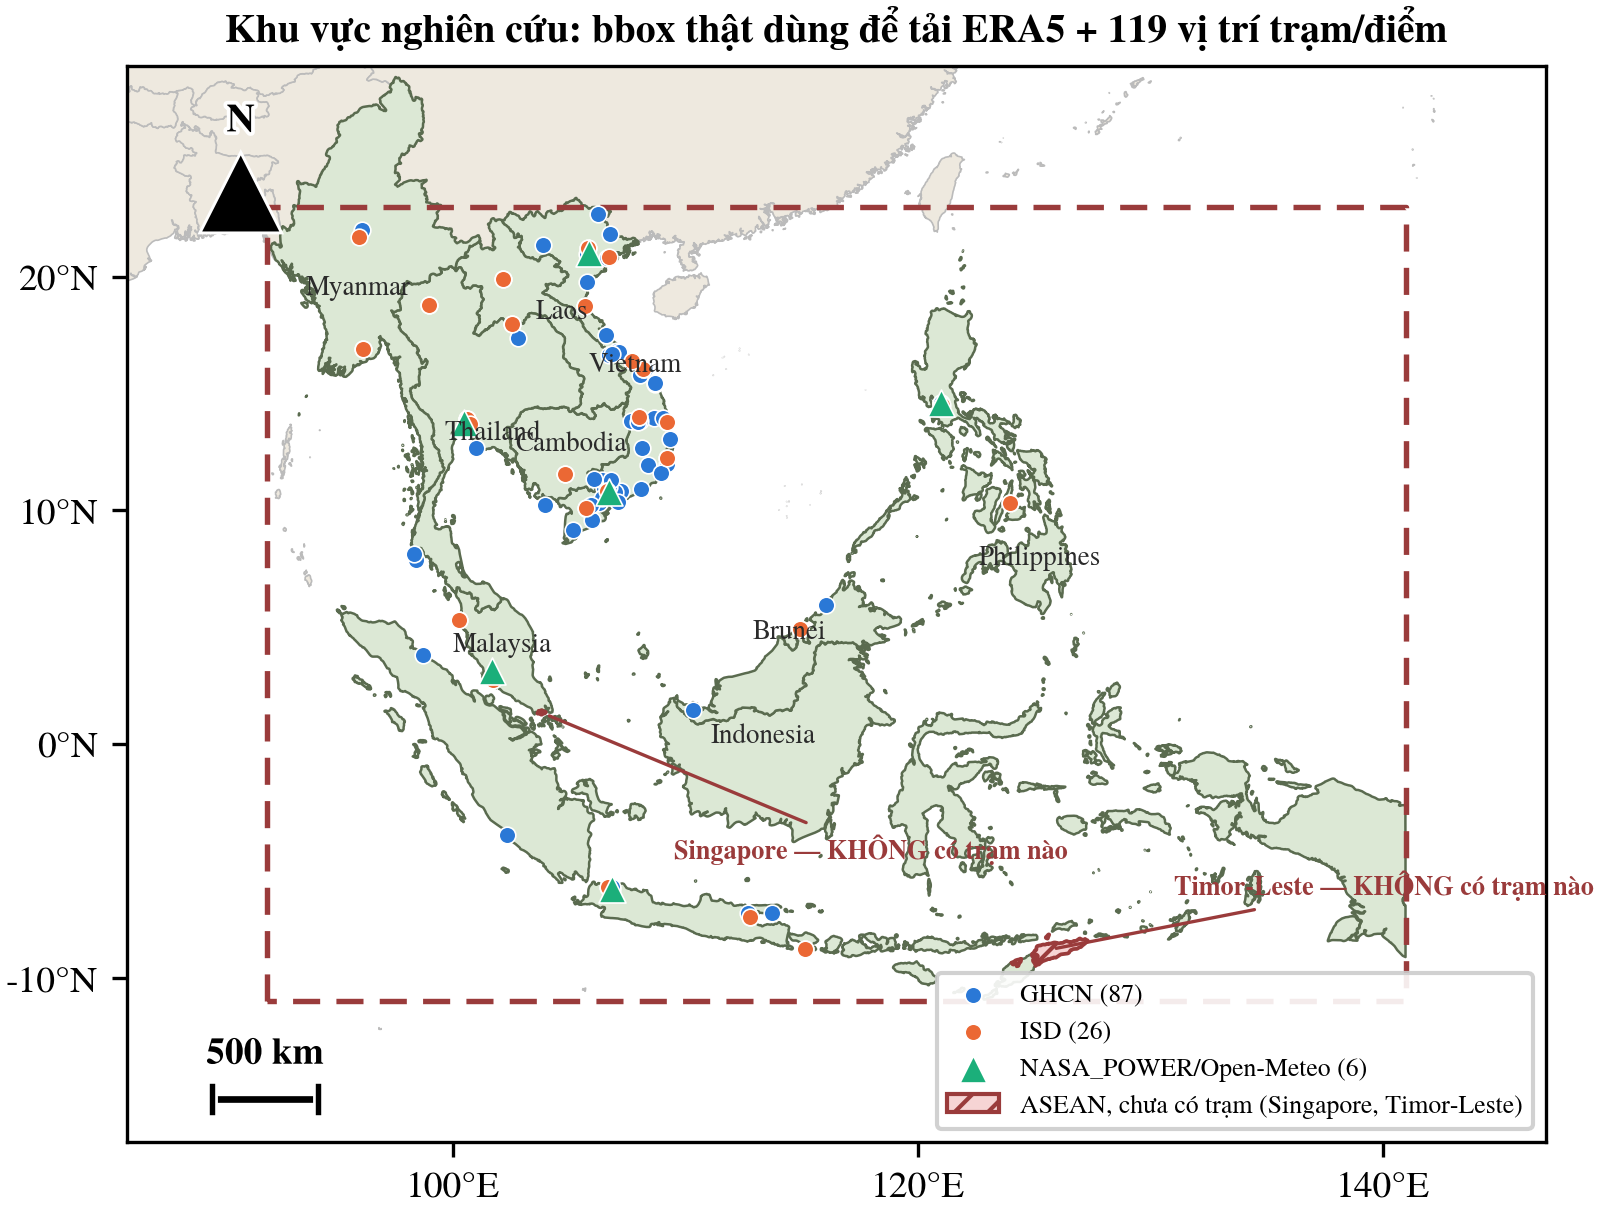
\includegraphics[max width=\linewidth]{figures/study_area_map.png}
\caption[Bản đồ khu vực nghiên cứu: bbox ERA5 và 119 vị trí trạm thật]{Khu vực nghiên cứu: khung nét đứt là bbox thật dùng để tải ERA5; 119 điểm là vị trí trạm/điểm thật, tô màu theo nguồn (GHCN 87, ISD 26, NASA POWER/Open-Meteo 6). Chín nước ASEAN tô xanh nhạt có ít nhất một trạm; Singapore và Timor-Leste (đánh số 1 và 2; Timor-Leste tô đỏ gạch chéo) nằm trong vùng bbox về mặt địa lý nhưng nhóm không chọn được trạm/điểm quan trắc nào tại hai nước này.}
\label{fig:study-area}
\end{figure}

Kết luận: bbox ERA5 phủ hình học đủ mười một nước, nhưng trạm thật chỉ phủ 9/11 nước. Singapore không có
trạm nào trong danh sách của nhóm (lãnh thổ nhỏ hơn nhiều so với một ô lưới $0{,}25°$); Timor-Leste gia
nhập ASEAN sau khi nhóm đã chốt phạm vi thu thập. Đây là giới hạn phủ dữ liệu, không phải lỗi mã; nếu
cần, phải lấy thêm từ nguồn ngoài năm nguồn hiện tại (ví dụ Meteorological Service Singapore).

\section{Ước tính dung lượng dữ liệu}

Bảng~\ref{tab:volume} là ước tính lập ở giai đoạn đề cương, từ số đo thực nghiệm (trạm) và hình dạng mảng thật (ERA5).

\begin{table}[H]
\centering
\caption{Ước tính dung lượng dữ liệu theo phạm vi đề xuất}
\label{tab:volume}
\begin{tabular}{@{}L{6cm}L{6.5cm}@{}}
\toprule
\textbf{Nguồn (phạm vi đề xuất)} & \textbf{Dung lượng} \\
\midrule
GHCN, 16 trạm VN, toàn lịch sử & 25,85 MB (đo thực nghiệm) \\
ISD, 10 trạm VN, 1 năm (2024) & 42,94 MB (đo thực nghiệm) \\
NASA POWER + Open-Meteo & Dưới 100 MB (truy vấn theo điểm) \\
ERA5 (ARCO), vùng ĐNA, 8 biến, 5 năm, tần suất giờ & Xấp xỉ 34,8 GB (tính từ hình dạng mảng thật: $1440 \times 721$ điểm lưới, kiểu \texttt{float32}) \\
\midrule
\textbf{Tổng ước tính} & \textbf{Xấp xỉ 35--36 GB} \\
\bottomrule
\end{tabular}
\end{table}

Khi tải thật (Mục~6.1), dữ liệu thô đạt 23,4~GB (ERA5 9 biến, 5 năm: 22~GB nén zlib; trạm/điểm 1,4~GB
do ISD mở rộng lên 10 năm). Sau khi nội suy ERA5 vào 113 điểm, kho \texttt{WeatherObs} chỉ còn 303~MB
Parquet (Bảng~\ref{tab:data-appendix}), vừa RAM một máy 36~GB. Spark được dùng vì bước nạp 22~GB Zarr
toàn cầu và để sẵn sàng mở rộng cho toàn lưới ERA5, không phải vì kho đã tích hợp vượt RAM; Mục~6.4
đo điểm hoà vốn giữa Spark và DuckDB trên cùng kho.

\section{Đánh giá theo tiêu chí 5V}

\textbf{Volume}: 23,4~GB thô, 303~MB sau tích hợp (Mục~4.3). \textbf{Variety}: ba dạng cấu trúc (lưới đa
chiều ERA5, bảng ``long'' GHCN, bản tin có trường nén ISD) và ba cú pháp (NetCDF/GRIB2, CSV, JSON).
\textbf{Velocity}: dữ liệu lịch sử, mô phỏng luồng bằng Kafka và Spark Structured Streaming.
\textbf{Veracity}: độ phủ trạm lệch giữa các nước và xung đột giữa nguồn trạm với nguồn mô hình, cần
Survivorship (Mục~3.3, 4.5). \textbf{Value}: phát hiện dị thường đã đối chứng với sự kiện thật
(Mục~6.8--6.10); ứng dụng nông nghiệp, năng lượng và UAV là hướng phát triển (Mục~9).

\section{Đặc trưng dữ liệu và yêu cầu xử lý}
\label{sec:data-characteristics}

Dữ liệu năm nguồn có ba nhóm vấn đề cần xử lý trước khi tích hợp: dữ liệu thiếu, giá trị ngoài
khoảng hợp lệ và đo lường không đồng nhất giữa các nguồn. Hình~\ref{fig:missing-rate} và
\ref{fig:outlier-rate} đo quy mô của hai nhóm đầu; Bảng~\ref{tab:sample-records} trích bản ghi thật
trước và sau xử lý bằng truy vấn DuckDB trên \texttt{data\_samples/} và kho \texttt{weatherobs.parquet}.

\subsection{Dữ liệu thiếu và giá trị bất thường theo biến, theo nguồn}

\begin{figure}[H]
\centering
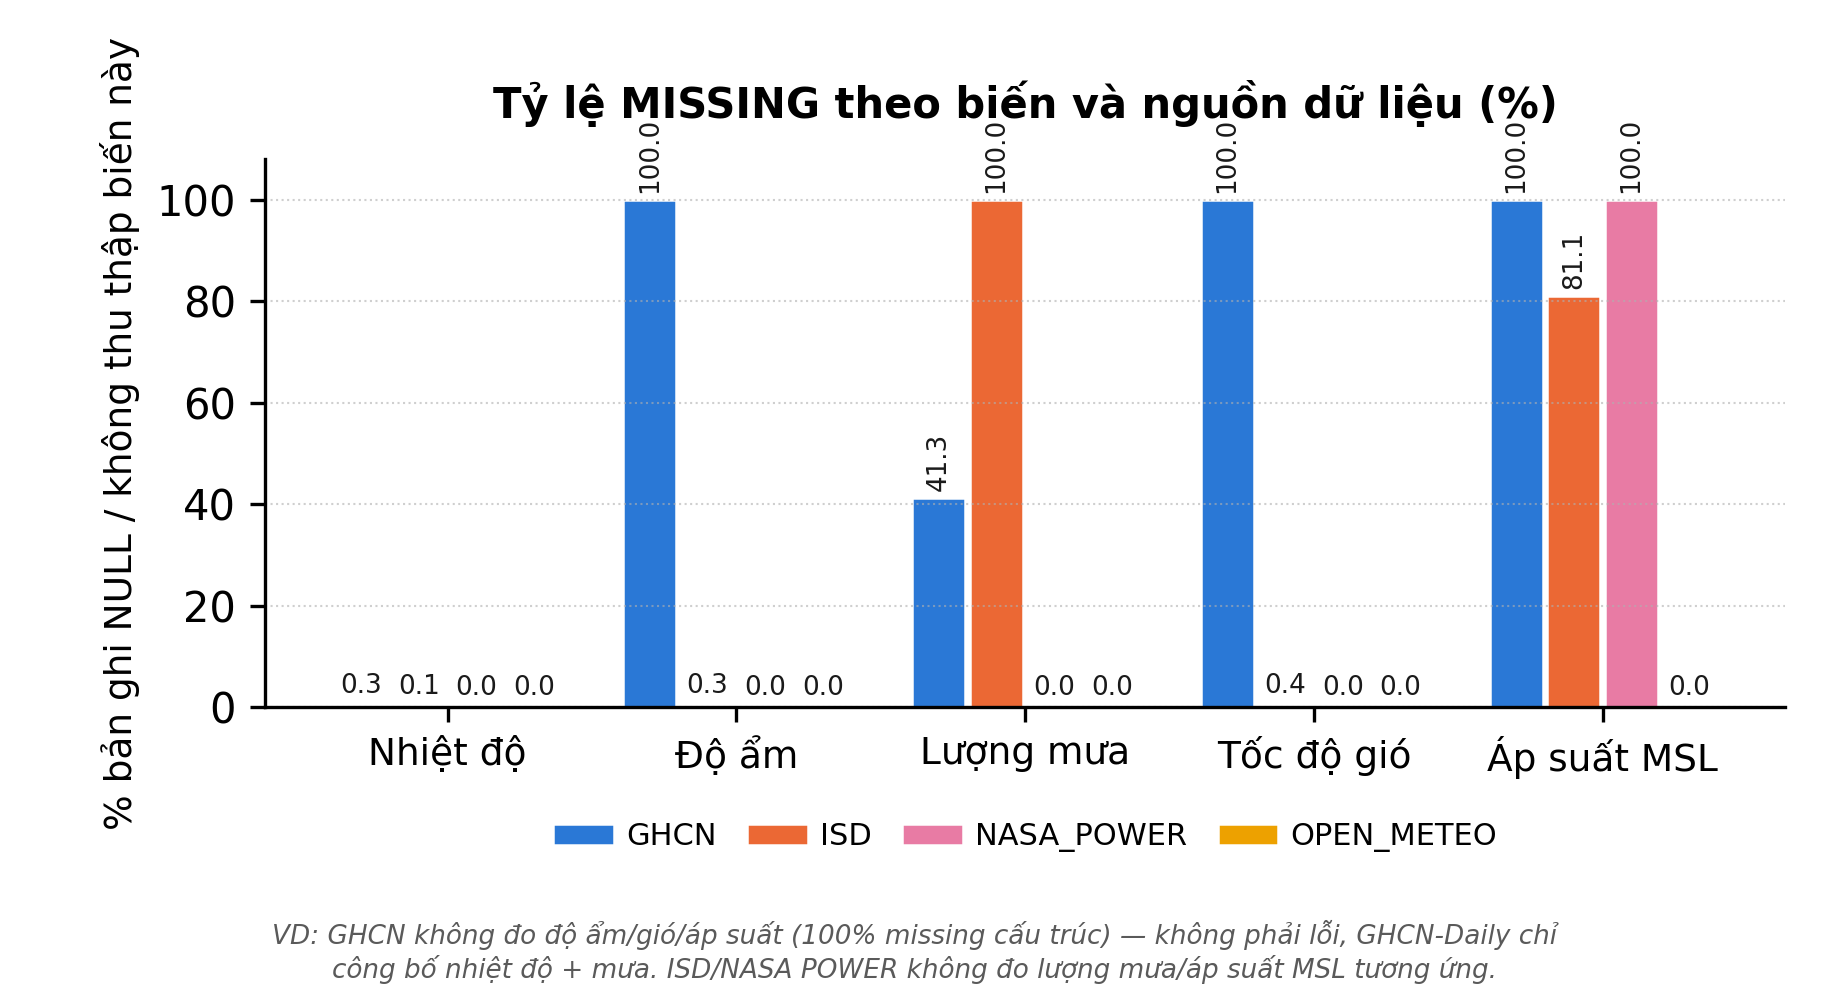
\includegraphics[width=0.78\linewidth]{figures/data_quality_missing_pct.png}
\caption[Tỷ lệ thiếu theo biến và nguồn]{Tỷ lệ thiếu (\%) theo biến và nguồn trên bốn nguồn điểm/trạm
(4.000.489 dòng: ISD 3.071.275, GHCN 655.164, Open-Meteo 263.088, NASA POWER 10.962). ERA5 không đưa
vào vì lưới đã nội suy đủ vào toạ độ trạm, luôn 0\% thiếu theo cấu trúc. Script:
\texttt{warehouse/plot\_data\_quality.py}.}
\label{fig:missing-rate}
\end{figure}

\begin{figure}[H]
\centering
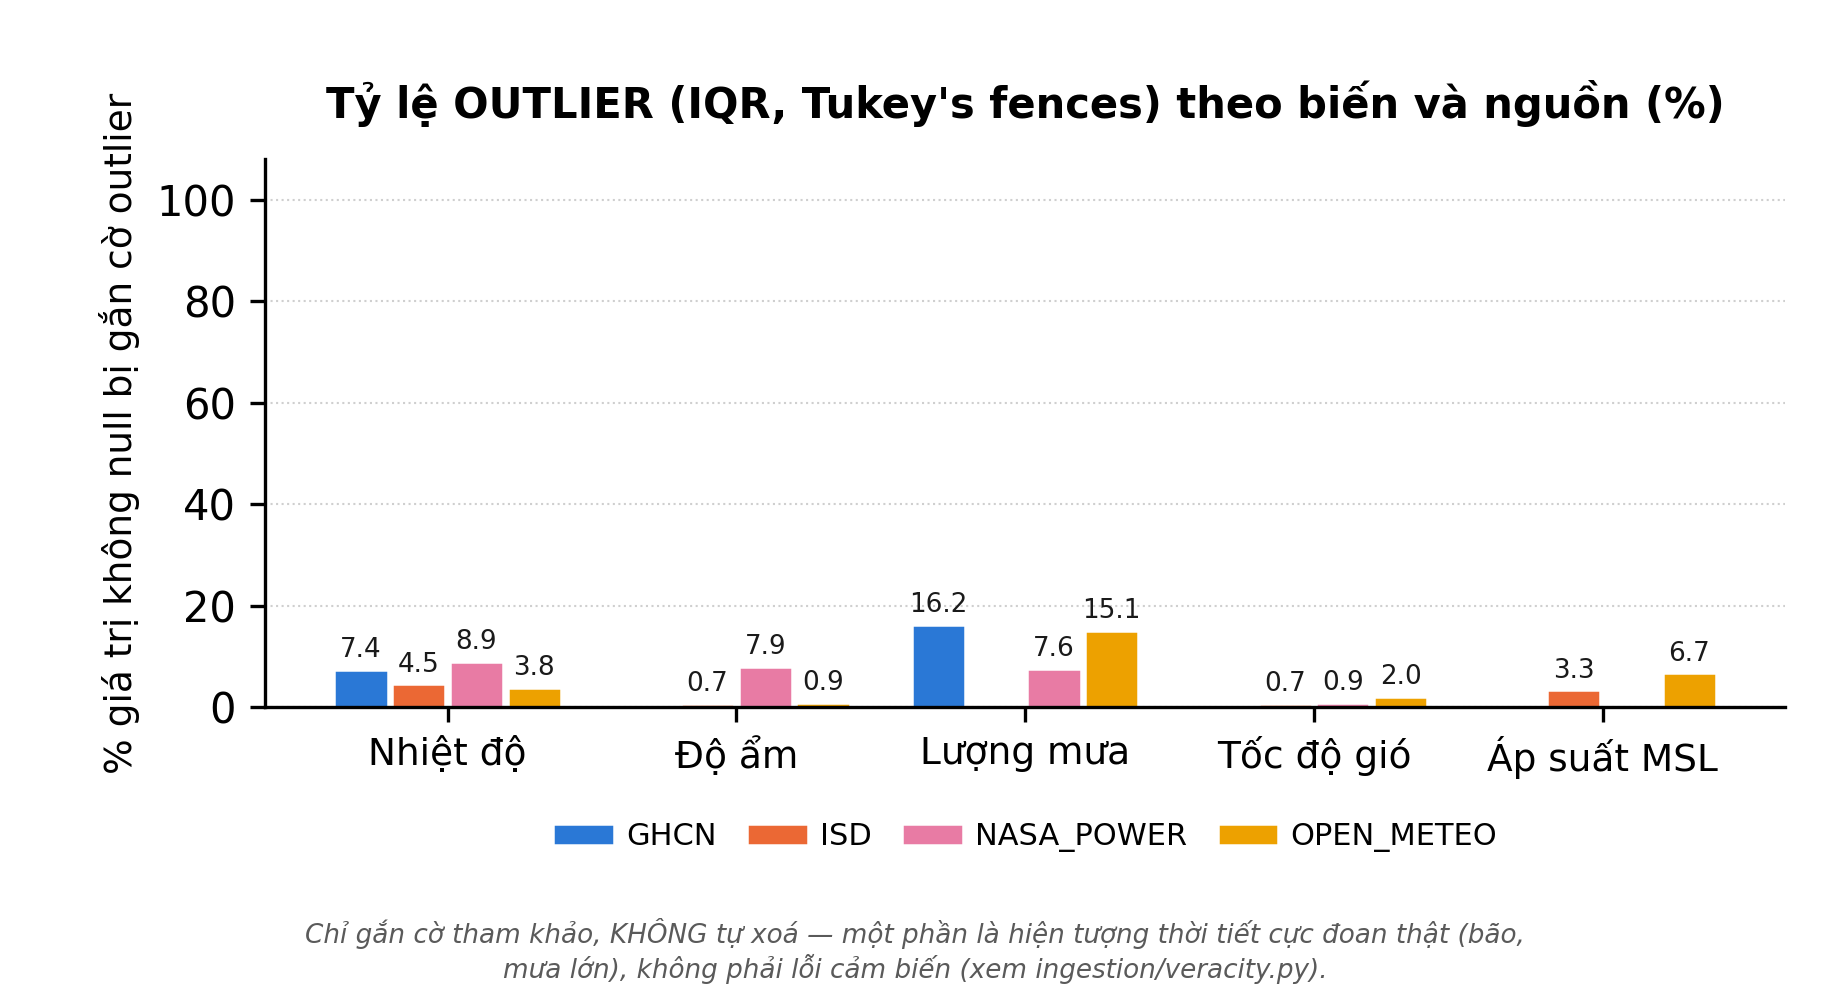
\includegraphics[width=0.78\linewidth]{figures/data_quality_outlier_pct.png}
\caption[Tỷ lệ outlier (IQR) theo biến và nguồn]{Tỷ lệ giá trị bị gắn cờ bất thường thống kê (IQR,
Tukey's fences) theo biến và nguồn, trên các giá trị không null. Chỉ gắn cờ tham khảo, không xoá
(\texttt{ingestion/veracity.py}).}
\label{fig:outlier-rate}
\end{figure}

Các cột thiếu 100\% là thiếu do cấu trúc nguồn chứ không phải thiếu theo thời gian: GHCN-Daily không
công bố độ ẩm, gió, áp suất; NASA POWER chỉ có áp suất bề mặt. Áp suất mực nước biển của ISD thiếu
81,1\% vì phần lớn bản tin METAR không mang trường này, chỉ SYNOP có (Mục~6.12). Mưa GHCN thiếu 41,3\%
nghĩa là trạm không báo PRCP, không phải 41,3\% số ngày không mưa. Tỷ lệ bất thường cao nhất rơi vào
lượng mưa (GHCN 16,2\%, Open-Meteo 15,1\%), phù hợp với phân bố lệch phải mạnh của mưa nhiệt đới.

\subsection{Bản ghi mẫu trước và sau xử lý}

\begin{table}[!htbp]
\centering\footnotesize
\caption{Bản ghi thật trước và sau xử lý cho ba nhóm vấn đề}
\label{tab:sample-records}
\begin{tabular}{@{}p{1.5cm}p{3.3cm}p{3.3cm}p{3.1cm}p{2.1cm}@{}}
\toprule
Nhóm & Nguồn, vị trí, thời điểm & Bản ghi gốc (nguyên văn) & Sau xử lý trong \texttt{WeatherObs} & Quy mô \\
\midrule
Missing &
ISD, trạm 48097099999 (Yangon), 1/1/2024 00:30 &
\texttt{SLP="99999,9"} &
\texttt{pressure\_msl\_hpa}\newline\texttt{= NULL} &
81,1\% dòng ISD (Hình~\ref{fig:missing-rate}) \\ \addlinespace[3pt]
Out of range &
GHCN, trạm RPW00041229, 29/1/1991 &
\texttt{TMAX="398"}, \texttt{Q\_FLAG="O"} (NOAA tự gắn cờ outlier) &
\texttt{temp\_c = NULL},\newline\texttt{qc\_flag=}\newline\texttt{'GHCN\_Q:TMAX=O'} &
406 giá trị GHCN bị loại (Mục~6.12) \\ \addlinespace[3pt]
Không đồng nhất (đơn vị) &
Open-Meteo, Hà Nội, 1/1/2024 00:00 &
\texttt{"wind\_speed\_10m": 4,9}, \texttt{"hourly\_units": \{"wind\_speed\_10m": "km/h"\}} &
\texttt{wind\_speed\_ms = 4,9 / 3,6 = 1,36} &
Toàn bộ 263.088 dòng Open-Meteo trong kho đầy đủ \\ \addlinespace[3pt]
Không đồng nhất (định nghĩa) &
GHCN, trạm BMM00048042, 16/2/1950 &
\texttt{TMAX="317"}, \texttt{TMIN="111"}, \texttt{TAVG="218"} (M\_FLAG=H) &
\texttt{temp\_c = 21,8}, \texttt{temp\_def='TAVG'} (≠ (31,7+11,1)/2 = 21,4) &
Lệch trung bình 0,25\,°C toàn kho (Mục~6.12) \\
\bottomrule
\end{tabular}
\end{table}

Hàng thứ tư là không đồng nhất về ngữ nghĩa: GHCN dùng \texttt{TAVG} đo trực tiếp khi có, nếu không
mới lấy $(TMAX+TMIN)/2$, và hai cách lệch nhau trung bình 0,25\,°C trên toàn kho. Nhóm không hiệu
chỉnh độ lệch này mà ghi định nghĩa vào cột \texttt{temp\_def}, để phân tích xu hướng (Mục~6.9) tự
quyết định. Bảng~\ref{tab:heterogeneity} liệt kê đầy đủ các đặc trưng không đồng nhất của bốn nguồn
điểm và cách xử lý, đọc trực tiếp từ \texttt{ingestion/parsers.py}.

{\footnotesize
\begin{longtable}{@{}L{1.7cm}L{6.4cm}L{6.1cm}@{}}
\caption{Đo lường không đồng nhất giữa 4 nguồn điểm: đặc trưng và yêu cầu xử lý bắt buộc}
\label{tab:heterogeneity} \\
\toprule
\textbf{Nguồn} & \textbf{Đặc trưng gây không đồng nhất} & \textbf{Xử lý bắt buộc} \\
\midrule
\endfirsthead
\toprule
\textbf{Nguồn} & \textbf{Đặc trưng gây không đồng nhất} & \textbf{Xử lý bắt buộc} \\
\midrule
\endhead
\bottomrule
\endfoot
GHCN & Định dạng LONG (1 dòng/biến/ngày); giá trị ở phần mười (1/10°C, 1/10mm) &
PIVOT thành 1 dòng/ngày; chia 10 \\
 & Nhiệt độ ngày là TAVG hoặc (TMAX+TMIN)/2 trong cùng một cột &
Gắn nhãn \texttt{temp\_def} (TAVG / TMAX\_TMIN\_MID) \\
 & \texttt{DATE} theo giờ địa phương, không phải UTC & Gán 00:00 UTC theo quy ước \\
NOAA ISD & Trường nén nhiều giá trị con dạng ``a,b,c'' (TMP, DEW, SLP, MA1, WND), đơn vị phần mười &
Tách từng sub-field theo vị trí kèm mã QC; chia 10 theo từng trường \\
 & Không có sẵn RH\% & Tính từ nhiệt độ và điểm sương theo Clausius--Clapeyron \\
 & Một quan trắc gửi trùng qua METAR (FM-15) và SYNOP (FM-12) &
Khử trùng, ưu tiên FM-15 rồi FM-12 \\
 & MA1 chứa cả áp suất trạm lẫn altimeter/QNH &
Chỉ lấy áp suất trạm; không dùng altimeter thay SLP (lệch $-0{,}4$ đến $+1{,}5$ hPa) \\
NASA POWER & Áp suất PS ở kPa; bức xạ ở MJ/m²/ngày & Nhân 10 ra hPa; $\times 10^6/86400$ ra W/m² \\
 & File cũ chỉ có gió 2m (WS2M) &
Ưu tiên WS10M, thiếu thì quy đổi theo hồ sơ gió logarit, gắn cờ \texttt{WIND\_2M\_TO\_10M} \\
 & Giá trị thiếu là sentinel $-999{,}0$ & Đọc \texttt{fill\_value} từ header JSON, thay bằng NaN \\
 & Nhiệt độ ngày là trung bình của sản phẩm mô hình & Gắn nhãn \texttt{temp\_def = DAILY\_MEAN} \\
Open-Meteo & Đơn vị gió đổi theo tham số API (km/h mặc định) &
Đọc \texttt{hourly\_units} rồi mới quy đổi \\
\end{longtable}
}

Chữ ``range'' trong đồ án mang ba nghĩa khác nhau. Khoảng vật lý hợp lệ (ví dụ nhiệt độ $-10$ đến
$50°$C, áp suất MSL 870 đến 1085\,hPa) là ranh giới tuyệt đối ở QC tầng 2 trước khi vào kho
(Mục~6.12). Khoảng bách phân vị (p95, p99 riêng từng trạm) được tính sau, để phát hiện mưa lớn và
cực đoan theo ETCCDI (Mục~6.8). Độ trải phân phối (mưa lệch phải mạnh, nhiệt độ gần đối xứng,
Mục~6.11) là căn cứ chọn $z$-score hay IQR/bách phân vị cho từng biến.

% ==========================================================
\chapter{Kế hoạch thực hiện}
% ==========================================================

\section{Đội hình dự án}

Nhóm 16 có ba thành viên: Ngô Văn Quang (Ingestion Lead: thu thập, làm sạch dữ liệu), Nguyễn Cao
Lương (Schema Lead: Mediated Schema, Record Linkage) và Trương Tuấn Nghĩa kiêm Spark/PINN Lead và
Dashboard/PM Lead (xử lý phân tán, PINN, trực quan hoá, điều phối).


\section{Tiến độ tổng thể}

Học phần có ba mốc chính thức: đề cương (5/10), báo cáo tiến độ (20/10) và báo cáo cuối kỳ (15/11).
Nhóm thêm ba mốc nội bộ (chốt nhóm 26/9, kiểm thử 27/10, hội tụ hệ thống 2/11) để chia nhỏ quãng
20/10--15/11. Hình~\ref{fig:gantt} và Bảng~\ref{tab:team-progress} trình bày tiến độ thật theo người.

\begin{figure}[H]
\centering
\resizebox{\textwidth}{!}{%
\begin{ganttchart}[
    vgrid, hgrid,
    x unit=0.3cm,
    y unit chart=0.55cm,
    bar height=0.55,
    bar/.append style={fill=hustblue!55},
    bar label font=\scriptsize,
    milestone/.append style={fill=badred},
    milestone label font=\scriptsize,
    title height=1,
    time slot format=isodate
    ]{2026-09-26}{2026-11-15}
    \gantttitlecalendar{year, month=shortname} \\
    \ganttbar{Quang -- script tải mẫu, 4 nguồn lõi}{2026-09-26}{2026-10-05} \\
    \ganttbar{Quang -- tải đủ 5 nguồn, QC 4 tầng, sửa 4 lỗi}{2026-10-20}{2026-11-15} \\
    \ganttbar{Lương -- Mediated Schema nháp}{2026-09-26}{2026-10-05} \\
    \ganttbar{Lương -- schema chính thức, ER, Survivorship}{2026-10-20}{2026-11-15} \\
    \ganttbar{Nghĩa -- dựng môi trường Spark/Docker}{2026-09-26}{2026-10-05} \\
    \ganttbar{Nghĩa -- cụm Spark+Kafka, dashboard khung}{2026-10-05}{2026-10-20} \\
    \ganttbar{Nghĩa -- PINN, tối ưu, dashboard 10 panel, báo cáo}{2026-10-20}{2026-11-15} \\
    \ganttmilestone{Chốt nhóm (nội bộ) 26/9}{2026-09-26} \\
    \ganttmilestone{Nộp đề cương (chính thức) 5/10}{2026-10-05} \\
    \ganttmilestone{Báo cáo tiến độ (chính thức) 20/10}{2026-10-20} \\
    \ganttmilestone{Kiểm thử (nội bộ) 27/10}{2026-10-27} \\
    \ganttmilestone{Hội tụ hệ thống (nội bộ) 2/11}{2026-11-02} \\
    \ganttmilestone{Báo cáo cuối kỳ (chính thức) 15/11}{2026-11-15}
\end{ganttchart}%
}
\caption{Tiến độ thật theo người: mỗi thanh là một sản phẩm đã hoàn thành trong đúng khoảng thời
gian đó (cùng dữ liệu với Bảng~\ref{tab:team-progress})}
\label{fig:gantt}
\end{figure}

\begin{table}[H]
\centering\footnotesize
\caption{Sản phẩm cụ thể theo người tại ba mốc chính thức}
\label{tab:team-progress}
\begin{tabular}{@{}L{2.6cm}L{1.3cm}L{6.3cm}L{3.2cm}@{}}
\toprule
\textbf{Người} & \textbf{Mốc} & \textbf{Sản phẩm} & \textbf{Bằng chứng} \\
\midrule
Ngô Văn Quang & 5/10 & Script tải GHCN/ISD/ERA5 mẫu, kiểm chứng 4 nguồn lõi & \path{check_data_sources.py} \\
Ngô Văn Quang & 20/10--15/11 & Tải đầy đủ 5 nguồn, QC 4 tầng, sửa 4 lỗi pipeline & \path{ingestion/}, Mục~6.12 \\
Nguyễn Cao Lương & 5/10 & Thiết kế Mediated Schema nháp & \texttt{archived/docs/06} \\
Nguyễn Cao Lương & 20/10--15/11 & Schema chính thức, Survivorship, Entity Resolution & \path{entity_resolution.py}, \path{survivorship.py} \\
Trương Tuấn Nghĩa & 5/10 & Dựng môi trường Spark, Docker & \path{docker-compose.*.yml} \\
Trương Tuấn Nghĩa & 20/10 & Cụm Spark+Kafka, dashboard khung, streaming cơ bản & Mục~6.6 \\
Trương Tuấn Nghĩa & 15/11 & PINN, tối ưu Spark, dashboard 10 panel, báo cáo/slide hoàn thiện & Mục~6.4--6.7 \\
\bottomrule
\end{tabular}
\end{table}

\section{Kế hoạch chi tiết theo tuần}

Mỗi tuần có một mốc kết thúc và mỗi hạng mục có tiêu chí hoàn thành (Definition of Done): tuần 1
tải mẫu, schema nháp, môi trường Spark (đến 5/10); tuần 2 tải batch đầy đủ, schema chính thức, cụm
Spark, streaming cơ bản (đến 20/10); tuần 3 xử lý outlier, Record Linkage, PINN nếu khả thi (đến 2/11);
tuần 4 chốt dữ liệu, hoàn thiện báo cáo và slide (đến 15/11).

\section{Chiến lược giảm tải cho vai trò kiêm nhiệm}

Vì một thành viên gánh gấp đôi khối lượng, nhóm áp dụng ba nguyên tắc: (1) PINN là hạng mục điểm
cộng có thể bỏ, phương án lùi là hồi quy MLlib thông thường; (2) điều phối dự án giữ ở mức tối thiểu
(roadmap và board công việc); (3) hai hạng mục bắt buộc là pipeline Spark chạy đúng và Dashboard đủ dữ
liệu thật được làm xong trước mọi hạng mục nâng cao.

% ==========================================================
\chapter{Kết quả thực nghiệm}
% ==========================================================

Mọi số liệu trong chương này lấy từ các lần chạy thật trên dữ liệu thật, đối chiếu với kiến trúc ở
Chương~3 và kế hoạch ở Chương~5. Chi tiết và script tái lập nằm tại \texttt{archived/docs/10} và
\texttt{archived/docs/14} trong kho mã nguồn.

\section{Quy mô dữ liệu đã tích hợp}

Bảng~\ref{tab:final-volume} là số bản ghi theo nguồn ở lần build cuối của kho
\texttt{weatherobs.parquet}.

\begin{table}[H]
\centering
\caption{Số bản ghi thật theo nguồn (tổng 8.955.313 dòng, sau kiểm soát chất lượng)}
\label{tab:final-volume}
\begin{tabular}{@{}L{4cm}R{2.4cm}L{6.8cm}@{}}
\toprule
\textbf{Nguồn} & \textbf{Số bản ghi} & \textbf{Phạm vi} \\
\midrule
ERA5 (CDS, nội suy Bilinear) & 4.954.824 & 113 trạm $\times$ 43.848 giờ (2020--2024), 9 biến \\
NOAA ISD/Global Hourly & 3.071.275 & 26 trạm, 10 năm 2015--2024, đã gộp bản tin trùng \\
GHCN-Daily & 655.164 & 41 trạm (VN + ĐNA), toàn lịch sử 1943--2026 \\
Open-Meteo Historical & 263.088 & 6 điểm đại diện, 2020--2024, theo giờ \\
NASA POWER & 10.962 & 6 điểm đại diện, 2020--2024, theo ngày \\
\bottomrule
\end{tabular}
\end{table}

Kho dữ liệu phủ 119 vị trí (113 trạm quan trắc thật, định danh qua bảng \textit{Location}) trên 9
quốc gia Đông Nam Á, đạt 100\% tính toàn vẹn tham chiếu (referential integrity) khi kiểm tra tự
động bằng bộ 83 unit/integration test đi kèm mã nguồn. Kho được ghi qua Spark thành 109 partition
(\texttt{year/source}), số dòng đọc lại khớp 100\% số dòng ghi vào; toàn bộ quá trình build mất
khoảng 3 phút.

Số trạm GHCN xuất hiện với bốn giá trị vì chúng đo bốn tập khác nhau: \textbf{87} trạm có trong
metadata chín nước, là tập ứng viên cho Entity Resolution (Hình~\ref{fig:study-area}, Mục~6.2);
\textbf{41} trạm trong số đó thực sự có dữ liệu trong kho (Bảng~\ref{tab:final-volume}); \textbf{27}
trạm trong 41 trạm có đủ $\geq 30$ năm nhiệt độ cho kiểm định Mann--Kendall (Mục~6.9). Như vậy
$27 \subseteq 41 \subseteq 87$. Riêng \textbf{61} (Mục~6.3) là số trạm thuộc mọi nguồn điểm có ít
nhất một cặp (vị trí, ngày) trùng ERA5, không lồng vào ba tập trên.

ERA5 đủ 540/540 tệp (9 biến $\times$ 60 tháng), mỗi biến đủ 43.848/43.848 giờ, 0\% giá trị thiếu,
khoảng giá trị hợp lý về vật lý (nhiệt độ $-0{,}4$ đến 46\textdegree{}C; áp suất thấp nhất 932~hPa và
gió khoảng 40~m/s tại tâm bão). Toàn bộ tải qua kênh CDS chính thức, cắt vùng phía máy chủ (Mục~4.1);
nút thắt là hàng đợi máy chủ (có yêu cầu chờ hơn một giờ), nên nhóm chạy song song hai tài khoản theo
hai chiều. Kênh ARCO chỉ dùng thử ban đầu: mỗi khối của nó chứa một giờ dữ liệu toàn cầu, nên lấy 22~GB
vùng Đông Nam Á phải tải khoảng 1~TB, xấp xỉ 27,8 giờ ở 10~MB/s. Script tải theo tháng và chạy tiếp
được sau khi bị ngắt.

\section{Giải quyết dị biệt định danh: Entity Resolution GHCN--ISD}

GHCN và ISD gán hai hệ mã độc lập cho cùng một trạm vật lý, nên không thể nối qua khoá
\texttt{location\_id}. Nhóm liên kết theo khoảng cách (Haversine, lân cận gần nhất 1--1, ngưỡng
5\,km), đúng kỹ thuật \textit{Record Linkage} dựa trên thuộc tính ở Chương~2: 22/26 trạm ISD
(84,6\%) khớp được một trạm GHCN, khoảng cách trung bình 0,53\,km, nhiều cặp trùng toạ độ tuyệt đối.

\textbf{Precision/recall theo nhãn số WMO.} Nhãn độc lập với toạ độ lấy từ số WMO: 5 chữ số cuối
của mã GHCN (\texttt{VMM00048820} $\to$ 48820) và 5 chữ số đầu của mã USAF khi USAF kết thúc bằng 0
(\texttt{48820099999} $\to$ 48820). Quy ước này cho 15 cặp, cách nhau 0--2,76\,km; chỉ 23/26 trạm ISD
gán được nhãn, và hai mã có thể cùng tra từ một danh bạ WMO. Cả 15/15 cặp nằm trong 22 cặp Haversine
và không cặp nào bị ghép sai (precision, recall 100\% trên tập có nhãn). Bốn trạm ISD không khớp
không trùng số WMO với trạm GHCN nào; riêng \texttt{48825199999} trùng 5 chữ số với một mã GHCN nhưng
cách 100,9\,km, tức là hai trạm khác nhau chứ không phải một cặp bị bỏ sót.

\textbf{Survivorship: hai lỗi phương pháp đã sửa.} Lần đo đầu cho 0\% xung đột áp suất, nhưng đó là
0 trên 0 nhóm so sánh được vì ERA5 khi ấy chưa tải đủ. Hàm gốc còn so sánh từng bản ghi giờ, nên
biến thiên trong ngày của ISD bị tính nhầm thành xung đột giữa các nguồn. Sau khi gộp mỗi nguồn về
một giá trị/ngày rồi mới so sánh giữa các nguồn, đo lại trên kho đủ 8.955.313 dòng
(Bảng~\ref{tab:survivorship-conflict}): xung đột từ 0,0\% ở áp suất mực nước biển (37.479 nhóm, nay
là số 0 có ý nghĩa) đến 91,6\% ở mưa do chu kỳ tích luỹ khác nhau (Mục~6.12); gió 44,6\% là biến đo
trực tiếp mà các nguồn bất đồng nhiều nhất.

\begin{table}[H]
\centering\footnotesize
\caption{Tỷ lệ xung đột Survivorship thật theo biến, đo trên kho đầy đủ 8.955.313 dòng}
\label{tab:survivorship-conflict}
\begin{tabular}{@{}L{2.9cm}L{5.6cm}R{1.5cm}R{1.3cm}R{1.1cm}@{}}
\toprule
\textbf{Biến} & \textbf{Nguồn có $\geq 2$ bản ghi thật} & \textbf{Nhóm so sánh} & \textbf{Xung đột} & \textbf{Tỷ lệ} \\
\midrule
Nhiệt độ & ERA5, GHCN, ISD, NASA POWER, Open-Meteo & 119.504 & 3.872 & 3,2\,\% \\
Độ ẩm & ISD, NASA POWER, Open-Meteo & 10.962 & 990 & 9,0\,\% \\
Mưa & ERA5, GHCN, NASA POWER, Open-Meteo & 41.529 & 38.053 & 91,6\,\% \\
Gió & ERA5, ISD, NASA POWER, Open-Meteo & 58.101 & 25.926 & 44,6\,\% \\
Áp suất bề mặt & ERA5, ISD, NASA POWER & 33.921 & 1.803 & 5,3\,\% \\
Áp suất mực nước biển & ERA5, ISD, Open-Meteo & 37.479 & 0 & 0,0\,\% \\
\bottomrule
\end{tabular}
\end{table}

\textbf{Bảng giá trị đã hợp giải thật.} Hàm \path{resolve_survivorship()} gốc lặp từng nhóm bằng
Python, mất 9 giờ 37 phút cho 1,08 triệu dòng, nên trước đây chưa từng sinh bảng kết quả. Bản viết lại
vector hoá bằng pandas chạy 8,96 triệu dòng trong 15 giây (\path{warehouse/survivorship_resolve.py}),
ghi \path{weatherobs_fused.parquet}: 856.452 dòng, đúng 1 dòng/vị trí/ngày, kèm cột nguồn được chọn và
cờ xung đột; đếm lại xung đột trên bảng này khớp tuyệt đối Bảng~\ref{tab:survivorship-conflict}. Ví dụ
Hà Nội (\texttt{VMM00048820}) ngày 7/9/2024: nhiệt độ 25,9\textdegree{}C lấy từ GHCN; mưa 8,48\,mm,
áp suất bề mặt 989,2\,hPa và mực biển 992,5\,hPa lấy từ ERA5 vì GHCN thiếu; không biến nào bị gắn cờ.

\subsection{Fellegi--Sunter, luật phủ quyết và liên kết trạm với lưới ERA5}
\label{sec:er-fs}

Ngưỡng 5\,km là một quyết định cứng. Nhóm chạy thêm mô hình Fellegi--Sunter~\cite{fellegi1969theory}
trên đúng 2.262 cặp ứng viên ($87 \times 26$, \path{warehouse/er_fellegi_sunter.py}) với ba đặc
trưng rời rạc hoá: khoảng cách (5 mức, từ $<1$ đến $\ge 100$\,km), chênh độ cao (4 mức) và độ giống
tên trạm. Số WMO không làm đặc trưng vì đó là nhãn đánh giá. Xác suất $m$, $u$ ước lượng bằng EM
không giám sát (80 vòng, tỷ lệ khớp tiên nghiệm $p = 0{,}0137$); trọng số $w = \sum\log_2(m/u)$, ví
dụ cách dưới 1\,km được $+10{,}99$, tên giống được $+11{,}42$. Ngưỡng theo định nghĩa gốc:
$\theta_h = 6{,}64$ ứng với tỷ lệ ghép nhầm $\mu \le 0{,}05\%$, $\theta_l = -1{,}31$ ứng với tỷ lệ
bỏ sót $\lambda \le 1\%$.

\textbf{Luật phủ quyết} áp trước khi chấm điểm, ngưỡng lấy từ dữ liệu: cặp khớp thật cách nhau tối
đa 2,76\,km và lệch độ cao tối đa 9,3\,m, nên nhóm đặt khoảng cách $>10$\,km, chênh độ cao $>100$\,m
và khác quốc gia. Ba luật loại tuần tự $1.625 + 608 + 1 = 2.234$ cặp, còn 28 cặp được chấm: 25
\emph{khớp}, 3 \emph{cần xem xét}; không cặp khớp thật nào bị loại. Luật chặn 2 cặp mà mô hình đã xếp
\emph{khớp} chỉ vì tên giống (\texttt{SURABAYA/PERAK}--\texttt{SURABAYA JUANDA}, 19,7\,km;
\texttt{MANDALAY}--\texttt{MANDALAY INTL}, 33,7\,km), đều là hai trạm khác nhau, cùng 53 cặp lẽ ra
rơi vào vùng cần xem xét.

\begin{table}[H]
\centering\footnotesize
\caption{Haversine và Fellegi--Sunter (FS) trên cùng hai tập nhãn WMO}
\label{tab:er-fs-compare}
\begin{tabular}{@{}L{4.6cm}R{1.0cm}R{1.4cm}R{2.3cm}R{2.3cm}R{1.3cm}@{}}
\toprule
\textbf{Phương pháp} & \textbf{Số cặp} & \textbf{Recall L15} & \textbf{Precision Lmeta} & \textbf{Recall Lmeta} & \textbf{Chưa có nhãn} \\
\midrule
Haversine 5\,km, 1--1 (hiện tại) & 22 & 15/15 & 17/17 (100\%) & 17/17 (100\%) & 5 \\
FS, \emph{khớp}, 1--1 & 22 & 14/15 & 16/16 (100\%) & 16/17 (94,1\%) & 6 \\
FS, \emph{khớp}, nhiều--một & 25 & 15/15 & 17/17 (100\%) & 17/17 (100\%) & 8 \\
\bottomrule
\end{tabular}
\end{table}

L15 là quy ước mã ở trên, chỉ dùng đo recall vì nhãn âm của nó không tin được. Lmeta lấy trường
\texttt{WMO\_ID} của danh bạ GHCN, gán nhãn cho 943 cặp với 17 cặp dương, vì mã dạng
\texttt{VMW000410xx} không mã hoá WMO (\texttt{VMW00041010} Nha Trang mang WMO 48877). Kết quả trung
thực (Bảng~\ref{tab:er-fs-compare}): FS \textbf{không chính xác hơn} Haversine, bằng ở biến thể
nhiều--một và kém một cặp ở biến thể 1--1, nơi mô hình chọn \texttt{THW00041001} (chuỗi 1964--1967)
thay cho \texttt{TH000048456} (1943--2025), dù cả hai đều là sân bay Don Mueang. Gộp thêm vùng cần
xem xét vào 1--1 sinh một cặp sai (Manila--NAIA); bỏ luật phủ quyết không đổi precision/recall nhưng
thêm một cặp chưa có nhãn.

Giá trị của FS nằm ở chỗ khác: trọng số có nghĩa xác suất, ngưỡng gắn với tỷ lệ lỗi tường minh thay
cho con số 5\,km chọn theo kinh nghiệm, và vùng xem xét thủ công chỉ còn 3 cặp. Mô hình còn lộ ra cấu
trúc nhiều--một mà ràng buộc 1--1 che mất: Đà Nẵng, Tân Sơn Nhất và Don Mueang đều có hai chuỗi GHCN
của cùng một sân bay. Luật Haversine 1--1 lại phụ thuộc thứ tự duyệt: ở Tân Sơn Nhất nó ghép
\texttt{VM000048900} (1,969\,km) dù \texttt{VMW00041008} gần hơn (0,336\,km); kết quả đúng nhãn,
nhưng do thứ tự chứ không do tiêu chí.

\textbf{Liên kết trạm với lưới, không gộp.} Trạm là một điểm đo, còn ô ERA5 là giá trị trung bình
của một ô $0{,}25°$ trên địa hình mô hình: hai thực thể khác nhau cùng quan trắc một hiện tượng. Vì
vậy nhóm ghi lại quan hệ thay vì hợp nhất: \path{warehouse/output/station_grid_link.parquet} nối 119
vị trí với tâm ô gần nhất (trung vị 9,42\,km), kèm độ cao địa hình ERA5 và độ lệch độ cao. Kho chưa
tải trường địa thế vị \texttt{z}~\cite{hersbach2020era5}, nên độ cao địa hình được ước lượng bằng
phương trình thuỷ tĩnh từ SP, MSL và T2m năm 2020; các ô biển khơi cho 0,2--1,8\,m, xác nhận cách
ước lượng dùng được.

Độ lệch độ cao trạm trừ ERA5 trải từ $-465{,}8$ đến $+303{,}9$\,m, 19/119 vị trí lệch quá 100\,m.
Trạm ISD Luang Prabang ở 291\,m trong khi ô ERA5 ở 749\,m, và trạm ấm hơn ERA5 trung bình
3,53\textdegree{}C. Trên 61 trạm có chuỗi bias nhiệt 2020--2024, bias theo độ lệch độ cao có độ dốc
$-5{,}66$\textdegree{}C/km ($r = -0{,}69$), gần gradient chuẩn $-6{,}5$\textdegree{}C/km
(Hình~\ref{fig:er-fs-grid}b); hiệu chỉnh theo gradient chuẩn giảm bias tuyệt đối trung bình từ 0,63
xuống 0,44\textdegree{}C. Phần lớn chênh lệch trạm--ERA5 là khác biệt về tính đại diện.

Gộp hai thực thể sẽ biến chênh lệch 3,5\textdegree{}C ở Luang Prabang thành một ``xung đột'' cần chọn
bên thắng. Bước xác nhận chéo dị thường (Mục~6.8) đã làm đúng kiểu liên kết: mỗi nguồn tính $z$ trên
khí hậu nền của chính nó tại cùng \texttt{location\_id}, nên độ lệch cố định triệt tiêu. Bảng hợp giải
thì chưa: tại 19 vị trí lệch quá 100\,m, 16.748/162.255 ngày (10,3\%) lấy nhiệt độ từ ERA5 khi trạm
thiếu mà chưa hiệu chỉnh độ cao. Đề xuất (chưa cài đặt): dùng bảng liên kết để hiệu chỉnh theo
gradient hoặc gắn cờ các giá trị thay thế này.

\begin{figure}[H]
\centering
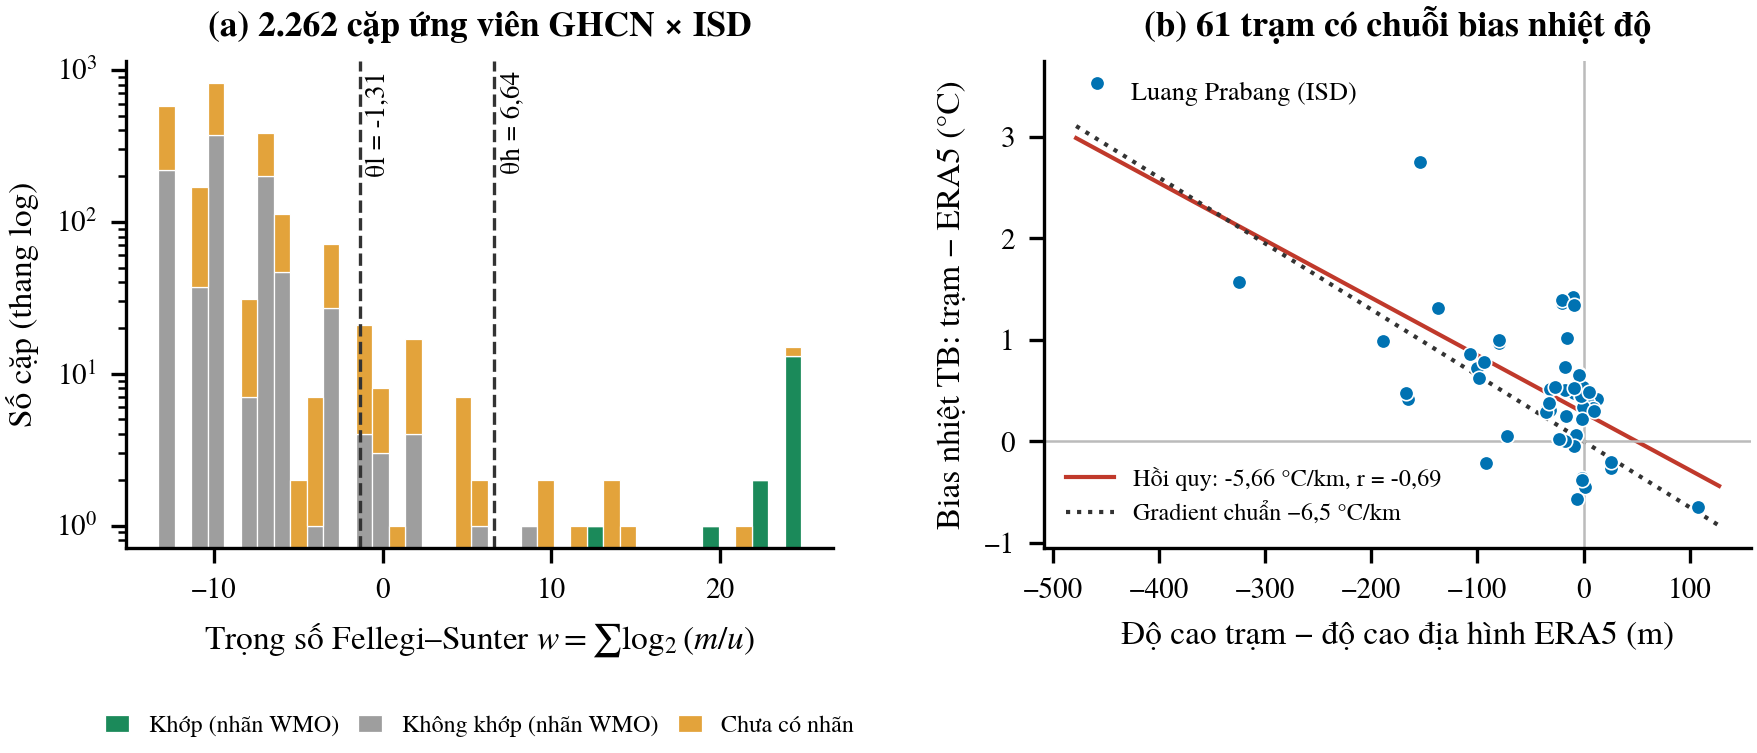
\includegraphics[max width=\linewidth]{figures/er_fs_station_grid.png}
\caption[Trọng số Fellegi--Sunter và độ lệch độ cao trạm--ERA5]{(a) Trọng số Fellegi--Sunter của
2.262 cặp \emph{trước} khi áp luật phủ quyết, tô theo nhãn WMO của danh bạ GHCN; đường đứt là
$\theta_l$ và $\theta_h$; cột xám bên phải $\theta_h$ là cặp Surabaya/Perak--Juanda, bị luật khoảng
cách chặn. (b) Độ lệch độ cao trạm trừ địa hình ERA5 so với bias nhiệt độ trung bình trạm trừ ERA5
(2020--2024, 61 trạm); đường đỏ là hồi quy, đường chấm là gradient chuẩn $-6{,}5$\textdegree{}C/km.}
\label{fig:er-fs-grid}
\end{figure}

\section{Kiểm chuẩn sai số nội suy không gian}

ERA5 nội suy Bilinear vào toạ độ trạm được so với giá trị trạm đo cùng ngày (trạm không làm đầu vào
nội suy). Trên 108.542 cặp nhiệt độ (61 trạm, 2020--2024), RMSE nhiệt độ 1,14\textdegree{}C (MAE
0,85\textdegree{}C), RMSE gió 1,05~m/s (MAE 0,78~m/s), chấp nhận được với lưới 0,25\textdegree{}. RMSE
mưa 19,83~mm (MAE 7,75~mm, 30.567 cặp), đúng hạn chế đã biết của tái phân tích với mưa (Chương~2). Sai
số nhiệt độ lớn nhất ở nhóm trạm cao nhất (0,99 / 0,94 / 1,42\textdegree{}C theo tercile độ cao), vì
lưới thô không nắm được địa hình chi tiết.

\section{Tối ưu hiệu năng Spark}

\texttt{cache()} giảm thời gian một truy vấn tổng hợp đại diện (nhiệt độ trung bình theo trạm/tháng,
GHCN) từ 0,36s xuống 0,11s (trung bình ba lần, kho 9,0 triệu dòng), cải thiện 69,4\%, vượt ngưỡng
30\%. Thêm \texttt{month} vào khoá partition giảm tỷ lệ partition lớn nhất từ 11,08\% xuống 0,94\%
nhưng tăng số partition 12 lần (109 $\to$ 1.306), làm nặng vấn đề tệp nhỏ. Đo lại (một lần làm nóng,
trung vị năm lần), dữ liệu đã partition vẫn chậm hơn 1,5--2,5 lần so với không partition trên bốn loại
truy vấn, vì Parquet đã lọc tốt nhờ thống kê min/max theo row-group còn 109 thư mục phát sinh chi phí
liệt kê tệp. Nhóm giữ chiến lược partition hiện tại; \textit{partition pruning} chỉ có lợi rõ ở quy mô
lớn hơn hoặc trên object storage.

\subsection{Thí nghiệm mở rộng quy mô: Spark so với một công cụ đơn máy}
\label{sec:scale-benchmark}

Để trả lời câu hỏi ``có thật sự cần Spark ở quy mô này'' (Mục~4.3), nhóm đo cùng truy vấn trên dữ
liệu nhân bản 1$\times$ đến 8$\times$ (655.164 $\to$ 5.241.312 dòng, bằng \texttt{UNION ALL}; dữ liệu
lặp làm nén và cache đẹp hơn thực tế) với Spark \texttt{local[1]}, \texttt{local[4]},
\texttt{local[*]} (14 core) và DuckDB, mỗi cấu hình một lần làm nóng và năm lần đo
(\texttt{warehouse/scale\_benchmark.py}).

\begin{figure}[H]
\centering
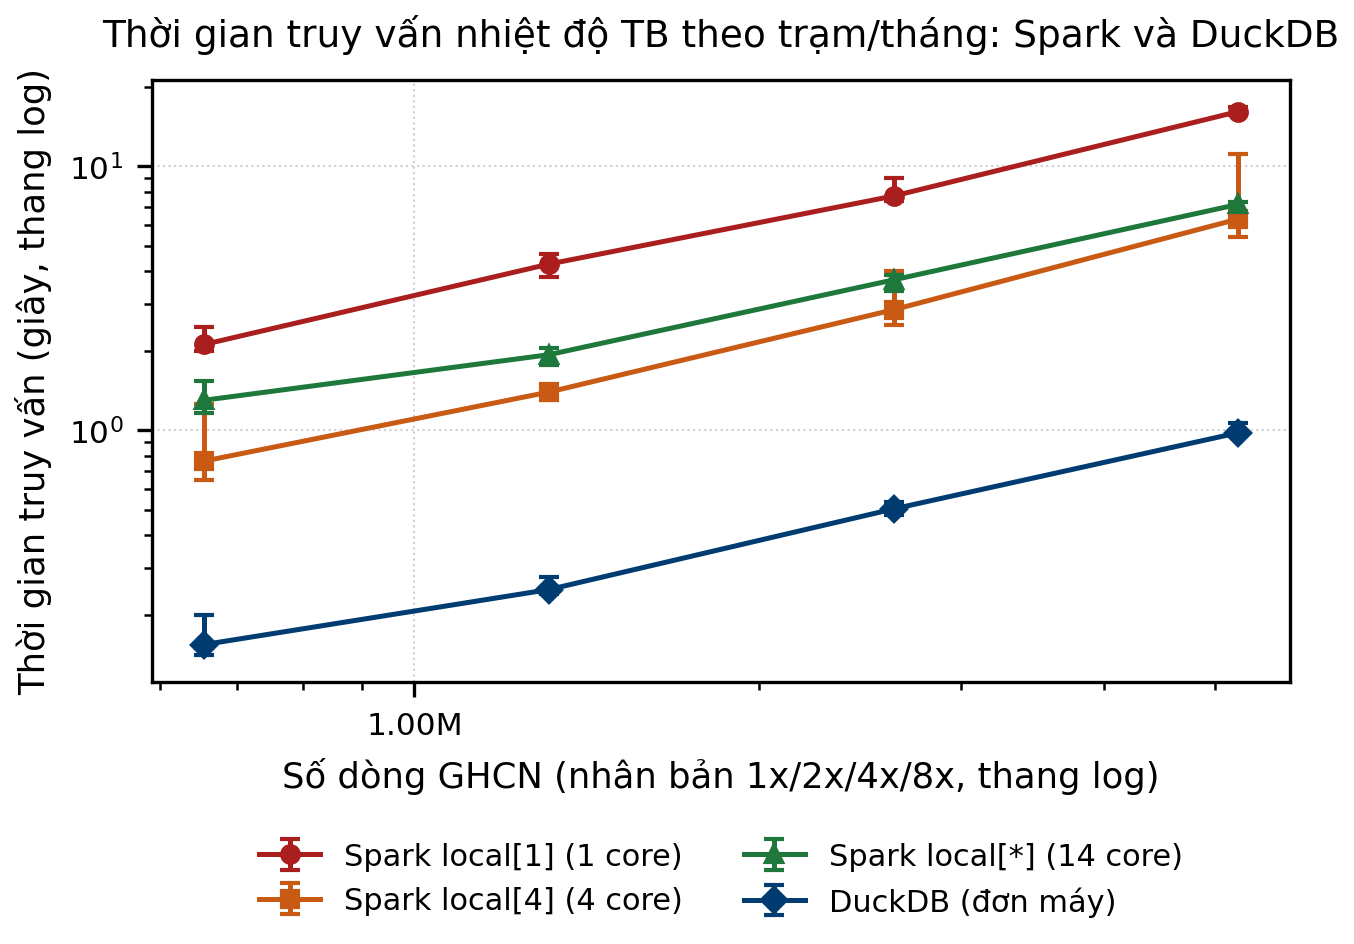
\includegraphics[max width=\linewidth]{figures/scale_benchmark.png}
\caption{Thời gian truy vấn trung vị (thang log-log) theo kích thước dữ liệu, 4 cấu hình}
\label{fig:scale-benchmark}
\end{figure}

Ở mọi mức (Hình~\ref{fig:scale-benchmark}), DuckDB nhanh hơn Spark \texttt{local[*]} 7,3--8,4 lần
(1$\times$: 0,155s so với 1,300s; 8$\times$: 0,979s so với 7,168s), và khoảng cách thu hẹp rất chậm,
nên điểm hoà vốn nằm xa ngoài phạm vi đã thử. Trong Spark, \texttt{local[*]} luôn chậm hơn
\texttt{local[4]} (8$\times$: 7,17s so với 6,31s): hiệu suất trên mỗi core chỉ 0,116--0,16 với 14 core
so với 0,64--0,76 với 4 core, tức chi phí điều phối vượt lợi ích song song. \texttt{local[4]} nhanh hơn
\texttt{local[1]} ổn định 2,6--3,1 lần. Dưới 10 triệu dòng, DuckDB nhanh hơn Spark; nhóm vẫn dùng Spark
vì mục tiêu học phần và để chuẩn bị cho toàn bộ lưới ERA5 (Mục~9).

\section{Mô hình học máy ràng buộc vật lý (PINN)}
\label{sec:pinn-full}

Hai mô hình PINN được huấn luyện trên dữ liệu thật, đều là mạng truyền thẳng nhỏ vì bài toán chỉ có
hai biến đầu vào và mục tiêu là minh chứng kỹ thuật physics loss.

\subsection{Mô hình (i): độ ẩm tương đối từ điểm sương}

\textbf{Bài toán.} Nhiều bản tin ISD chỉ có điểm sương, không có RH\%. Pipeline sản xuất tính RH\%
trực tiếp bằng Clausius--Clapeyron (\texttt{parsers.py}, Mục~3.2); mô hình (i) là thí nghiệm bổ sung:
mạng dự đoán RH\% từ $(T, T_d)$, có physics loss ép tuân thủ phương trình đó.

\begin{sloppypar}
\textbf{Kiến trúc.} Lớp \texttt{RHNet} (tệp \path{model/pinn_rh_from_dewpoint.py}): 2 đầu vào
$(T, T_d)$ $\to$ \texttt{Linear(2,16)} $\to$ Tanh $\to$ \texttt{Linear(16,16)} $\to$ Tanh $\to$
\texttt{Linear(16,1)} $\to$ Sigmoid $\to$ nhân 100: 2 lớp ẩn 16 nơ-ron, Tanh ở lớp ẩn, Sigmoid ở đầu ra
để ép RH\% về $(0,100)$.
\end{sloppypar}

\textbf{Phương trình vật lý.} Áp suất hơi bão hoà theo Clausius--Clapeyron (xấp xỉ Magnus):
\begin{equation}
e_s(T) = 6{,}112 \exp\!\left(\frac{17{,}67\,T}{T + 243{,}5}\right) \quad \text{(hPa, } T \text{ tính bằng } ^\circ\text{C)}
\end{equation}
Theo định nghĩa $\mathrm{RH} = 100 \times e_s(T_d)/e_s(T)$; physics loss ép đầu ra thoả định nghĩa này:
\begin{equation}
\mathcal{L}_{phys} = \frac{1}{N}\sum_i \left[\left(\frac{\widehat{\mathrm{RH}}_i}{100}\, e_s(T_i) - e_s(T_{d,i})\right)^2\right] \Big/ \overline{e_s(T_d)}^2, \qquad
\mathcal{L} = \mathcal{L}_{data} + 0{,}1\,\mathcal{L}_{phys}
\end{equation}
(chia cho bình phương trung bình $e_s(T_d)$ để physics loss không thứ nguyên).

\textbf{Huấn luyện và kết quả.} Adam, tốc độ học $5\times10^{-3}$, 200 epoch, 5.000 bản ghi ISD thật;
nhãn RH\% lấy từ chính công thức C-C vì ISD không có RH\% đo trực tiếp. Hàm mất mát giảm từ 1068 xuống
2,9, MAE cuối 1,07 điểm phần trăm: tốt cho mục đích minh chứng, nhưng không thay được công thức trực
tiếp (rẻ hơn, chính xác tuyệt đối).

\subsection{Mô hình (ii): trường gió hai chiều}

\textbf{Kiến trúc} (\texttt{model/pinn\_wind\_field\_v2.py::WindFieldNet}): 2 đầu vào $(lon, lat)$ đã
chuẩn hoá $\to$ \texttt{Linear(2,32)} $\to$ Tanh $\to$ \texttt{Linear(32,32)} $\to$ Tanh $\to$
\texttt{Linear(32,2)} $\to$ $(u,v)$: 2 lớp ẩn 32 nơ-ron, Tanh, lớp ra tuyến tính vì vận tốc không bị
chặn miền giá trị.

\textbf{Phương trình vật lý} (phương trình liên tục 2D, bảo toàn khối lượng cho chất lỏng không nén):
\begin{equation}
\frac{\partial u}{\partial x} + \frac{\partial v}{\partial y} = 0,
\qquad
\mathcal{L}_{phys} = \overline{\left(\frac{\partial u}{\partial x} + \frac{\partial v}{\partial y}\right)^{2}},
\qquad
\mathcal{L} = \mathcal{L}_{data} + \lambda\,\mathcal{L}_{phys}
\end{equation}
với đạo hàm riêng tính bằng \texttt{torch.autograd.grad} qua đồ thị của mạng, không dùng sai phân.

\textbf{Huấn luyện.} Adam, tốc độ học $10^{-3}$, 300 epoch, 113 trạm có gió ERA5 trung bình vector
15--17/6/2021 (91 trạm luyện, 22 trạm kiểm tra, seed cố định), quét
$\lambda \in \{0;\,0{,}01;\,0{,}1;\,1{,}0\}$. Tiền xử lý đổi từng bản ghi sang $(u,v)$ rồi mới lấy
trung bình theo trạm; bản cũ lấy trung bình cộng hướng gió theo độ, sai với đại lượng vòng tròn
($350^\circ$ và $10^\circ$ cho ra $180^\circ$), lỗi do Ngô Văn Quang phát hiện ngày 10/11/2026.

\textbf{Kết quả.} Trên tập kiểm tra, hồi quy thuần ($\lambda=0$) đạt RMSE \textbf{1,0473}, tốt hơn PINN
tốt nhất ($\lambda=0{,}1$, RMSE 1,0577). Data Loss hội tụ gần như giống nhau giữa hai $\lambda$, nhưng
Physics Loss ở $\lambda=0{,}1$ tăng từ $\approx$0,002 lên $\approx$0,14 rồi chững lại: mạng khởi tạo
gần như hằng số nên độ phân kỳ ban đầu gần 0 một cách ngẫu nhiên, và khi mạng học biến thiên không gian
thật thì độ phân kỳ xuất hiện, còn $\lambda=0{,}1$ quá yếu để ép nó về 0.

Kết luận: \textbf{với một lát cắt không-thời gian, không có chuỗi thời gian, PINN chưa vượt baseline}.
Giá trị của physics loss ở quy mô này là đảm bảo tính hợp lý vật lý của đầu ra, chưa phải giảm sai số;
đây là câu hỏi mở (Mục~\ref{sec:contributions}). Kết quả tái lập được: cài lại môi trường từ
\texttt{requirements.txt} cho RMSE giống hệt đến bốn chữ số thập phân.

\subsection{Mức độ toàn diện: PINN giải quyết được bao nhiêu trường dữ liệu?}

PINN chỉ chạm \textbf{2 trong 12 trường} của lược đồ \texttt{WeatherObs}: độ ẩm tương đối
(\texttt{rh\_pct}) và gió (tốc độ và hướng). Mười trường còn lại nội suy bằng Bilinear thuần
(Mục~6.6). Đây là lựa chọn có chủ đích, vì kế hoạch xếp PINN vào hạng mục tuỳ chọn (Mục~2.4).
Bảng~\ref{tab:pinn-summary} tóm tắt yêu cầu tính toán, đầu ra và kết quả đo được của hai mô hình.

\begin{table}[H]
\centering\footnotesize
\caption{Hai mô hình PINN: yêu cầu tính toán, đầu ra và kết quả đo được}
\label{tab:pinn-summary}
\begin{tabular}{@{}L{2.6cm}L{5.6cm}L{5.6cm}@{}}
\toprule
& \textbf{(i) RHNet: độ ẩm từ điểm sương} & \textbf{(ii) WindFieldNet: trường gió 2D} \\
\midrule
Dữ liệu vào & 5.000 bản ghi ISD thật, đầu vào $(T, T_d)$ & 113 trạm, gió ERA5 trung bình vector 15--17/6/2021; 91 luyện, 22 kiểm tra \\
Kiến trúc & 2--16--16--1, Tanh, đầu ra Sigmoid$\times$100; \textbf{337 tham số} & 2--32--32--2, Tanh, đầu ra tuyến tính $(u,v)$; \textbf{1.218 tham số} \\
Ràng buộc vật lý & Clausius--Clapeyron (6.1), hệ số 0,1 & Liên tục $\partial_x u + \partial_y v = 0$ (6.3), đạo hàm bằng autograd \\
Huấn luyện & Adam, lr $5\times10^{-3}$, 200 epoch & Adam, lr $10^{-3}$, 300 epoch, quét $\lambda \in \{0;\,0{,}01;\,0{,}1;\,1\}$ \\
Đầu ra & RH\% dự đoán cho từng bản ghi & \path{pinn_wind_field_output.parquet}: 113 dòng, $u,v$ dự đoán/quan trắc, phần dư, $\lambda=0{,}1$ \\
Kết quả & Loss 1068 $\to$ 2,9; MAE 1,07 điểm \% & RMSE kiểm tra: $\lambda=0$ đạt 1,0473, PINN tốt nhất 1,0577 \\
Giải quyết được & Trường \texttt{rh\_pct} cho 3.063.576 bản ghi ISD chỉ có điểm sương; mạng học lại đúng phương trình C--C & Điền gió tại điểm chưa có số liệu (thử trên 22 vị trí giữ lại: RMSE 1,06~m/s, sai số còn cao); phần dư đánh dấu 4 vị trí gió lệch trường vật lý $>$2,62~m/s \\
Chưa giải quyết & Nhãn sinh từ chính công thức, chưa có RH\% đo độc lập & PINN chưa thắng hồi quy thuần; chưa có chiều thời gian \\
\bottomrule
\end{tabular}
\end{table}

\textbf{PINN giải quyết được gì cho bài toán dị thường?} Bộ dò ở Mục~6.8 làm việc trên nhiệt độ và áp suất
(22.446 giá trị gắn cờ trong 2020--2024); PINN phủ thêm \textbf{2/12 trường} mà bộ dò chưa chạm tới, nên mở
rộng phạm vi phát hiện thay vì trùng lặp. Mô hình (i) cho trường \texttt{rh\_pct} ở 3.063.576 bản ghi ISD chỉ có
điểm sương, sai số 1,07 điểm \%. Mô hình (ii) nhận vào toạ độ nên \textbf{điền được gió} tại bất kỳ điểm nào
giữa các ô lưới ERA5 hoặc tại trạm thiếu số liệu; trên 22 vị trí giữ lại không dùng để luyện, RMSE là 1,06~m/s
so với tốc độ gió trung bình 2,26~m/s, tức sai số còn cao và cần thêm chiều thời gian. Cũng ở mô hình (ii), phần dư giữa gió quan trắc và trường PINN (trung bình
1,03~m/s) đánh dấu \textbf{4/113 vị trí} lệch quá 2,62~m/s (trung bình + 2$\sigma$): Mandalay (cả mã ISD
48600199999 và GHCN BMM00048042), Đồng Hới và Phú Quốc, đều là thung lũng, ven biển hoặc đảo. Đây là các ứng
viên \emph{dị thường gió cục bộ} mà phép $z$ trên nhiệt độ, áp suất không thấy; trạm ISD Mandalay cũng nằm trong
nhóm nhiều cờ QC nhất (Mục~6.12).

Bước tiếp theo có chỉ tiêu đo được: 93,3\% trong 5.910 ca tại trạm đã được ERA5 hoặc trạm lân cận xác nhận
(Hình~\ref{fig:anomaly-confirmation}), còn 375 ca \emph{dị thường cục bộ} (6,3\%) mà lưới ERA5 khoảng 28~km
không bắt được. Một trường PINN cho nhiệt độ và áp suất, phân giải cao hơn và nhất quán vật lý giữa các trạm,
sẽ dùng để phân xử các ca này; chỉ tiêu là số ca cục bộ giảm mà tỉ lệ nghi lỗi không tăng giả.

\textbf{Hướng phát triển và các công trình liên quan.} Kashinath và cộng sự~\cite{kashinath2021physics}
tổng hợp mười ca áp dụng ML có ràng buộc vật lý cho thời tiết và khí hậu. Bihlo và
Popovych~\cite{bihlo2022pinn} giải phương trình nước nông trên mặt cầu bằng PINN, đúng loại ràng
buộc có thời gian mà mô hình (ii) đang thiếu. GraphCast~\cite{lam2023graphcast} và
FourCastNet~\cite{pathak2022fourcastnet} học trực tiếp từ ERA5 ở quy mô toàn cầu, cho mốc so sánh
nếu mở rộng. Nhóm dự định ba bước: thêm chiều thời gian cho mô hình (ii), đối chiếu mô hình (i) với
RH\% độc lập của NASA POWER/Open-Meteo, rồi dùng PINN phân xử các ca dị thường cục bộ (Mục~\ref{sec:future-work}).

\section{Hạ tầng tính toán phân tán}

Cụm Spark ba node (một master, hai worker) và một Kafka broker chạy bằng Docker Compose: Spark Master
xác nhận hai worker \texttt{ALIVE}, một tác vụ thật (tổng 0 đến 999.999) chạy phân tán cho kết quả
đúng, Kafka consumer đọc lại đúng bản ghi JSON producer đã phát. Spark Structured Streaming đọc từ
Kafka (\texttt{spark\_streaming\_consumer.py}) tính đúng nhiệt độ trung bình theo trạm trên cửa sổ
trượt một phút, bước 30 giây. Hạ tầng được dựng lại trên Linux bằng image chính thức
\texttt{apache/spark:4.2.0} và \texttt{apache/kafka:3.7.0} sau khi image Bitnami bị gỡ khỏi Docker Hub.

Phát hiện dị thường theo luồng (\path{warehouse/spark_streaming_anomaly.py}) lấy tối đa 150 bản ghi mỗi
micro-batch, join tĩnh với khí hậu nền tính bằng batch (Mục~6.8), tính $z$ và cảnh báo $|z| \ge 2$.
Phát lại đợt nắng nóng 1/4--15/5/2024 (1.407 bản ghi) cho 179 cảnh báo qua 10 micro-batch, khớp 179/179
với batch và cùng giá trị $z$, vì hai đường dùng chung logic. Cấu hình:
\texttt{trigger(processingTime="3 seconds")}, \texttt{shuffle.partitions=4} (tránh 200 task rỗng mặc
định), checkpoint cục bộ. Không dùng watermark vì dữ liệu phát lại gán \texttt{event\_time} bằng giờ xử
lý; ngữ nghĩa đạt gần \emph{at-least-once}, chưa thử kill driver giữa chừng.

\begin{sloppypar}
Spark batch (Mục~6.1--6.4, 6.8--6.12) chạy \texttt{local[*]} trên máy 14 nhân,
\texttt{driver.memory=4g}, shuffle và AQE theo mặc định Spark 4.2.0 (Mục~\ref{sec:infra-limits}).
Kiểm thử thật phát hiện hai sự cố môi trường: Spark không khởi tạo được vì tên máy phân giải sang địa
chỉ LAN (sửa bằng \texttt{SPARK\_LOCAL\_IP}), và connector Kafka cố định 4.0.0 không tương thích PySpark
4.2.0 (\texttt{NoSuchMethodError}; sửa bằng cách lấy phiên bản connector theo môi trường cài đặt).
\end{sloppypar}

\section{Trực quan hoá và cảnh báo}

Dashboard Streamlit đọc trực tiếp kho Parquet (9,0 triệu bản ghi) với mười thành phần: chuỗi thời gian
theo trạm, tổng hợp theo nguồn, bản đồ có thanh trượt thời gian, so sánh NASA POWER với Open-Meteo
(2020--2024), cảnh báo bất thường theo IQR, đầu ra PINN trường gió, dị thường khí hậu (bản đồ $z$, đợt
nóng, SPI-3, mưa cực đoan; Mục~6.8), xu hướng dài hạn (Mục~6.9), trôi cảm biến (Mục~6.10) và cảnh báo
theo luồng. Bảng trung bình ngày được tính sẵn và cache nên đổi ngày hoặc trạm mất khoảng 0,6 giây. Cả
mười thành phần đã được chạy thật trên trình duyệt, không có lỗi runtime.

\section{Phát hiện dị thường khí hậu}

\path{warehouse/anomaly_detection.py} phát hiện dị thường khí hậu, mục tiêu chính của đề tài, theo chuẩn
khí tượng thay vì ngưỡng tự đặt. Spark gộp 9,0 triệu bản ghi thành 977.239 ngày--vị trí--nguồn
(nguồn theo giờ phải phủ đủ bốn khối 6 giờ mỗi ngày), rồi tính khí hậu nền theo ngày-trong-năm với cửa sổ
trượt $\pm$15 ngày; nền của GHCN là chuẩn WMO 1991--2020. Nhiệt độ và áp suất dùng dị thường chuẩn hoá
$z$ ($|z|\ge2$ bất thường, $|z|\ge3$ cực đoan); lượng mưa không có phân bố chuẩn nên dùng SPI~\cite{mckee1993spi}
và các chỉ số ETCCDI (Bảng~\ref{tab:anomaly-standards}).

\textbf{Cửa sổ kết quả là 2020--2024}: giai đoạn cả năm nguồn cùng có dữ liệu và có ERA5 để xác nhận chéo.
Chuỗi GHCN dài chỉ dùng làm khí hậu nền và cho xu hướng 30 năm ở Mục~6.9. Trong cửa sổ có 588.888 giá trị
ngày có nền; hệ thống gắn cờ 22.446 giá trị (3,8\%), gồm 20.627 bất thường và 1.819 cực đoan, trong đó
nhiệt độ 12.209 và áp suất 10.237. Theo nguồn: ERA5 15.283, ISD 3.241, GHCN 2.669, Open-Meteo 848, NASA
POWER 405. Bảng~\ref{tab:anomaly-events} đối chiếu kết quả với bốn sự kiện có thật.

{\footnotesize
\begin{longtable}{@{}L{1.3cm}L{2.7cm}L{3.0cm}L{4.4cm}L{2.4cm}@{}}
\caption[Các loại dị thường khí hậu đã triển khai]{Các loại dị thường khí hậu đã triển khai (xu hướng dài hạn và trôi cảm biến: Mục~6.9, 6.10)}
\label{tab:anomaly-standards} \\
\toprule
\textbf{Nhóm} & \textbf{Loại dị thường} & \textbf{Biến đầu vào} & \textbf{Tiêu chuẩn / ngưỡng} & \textbf{Nguồn} \\
\midrule
\endfirsthead
\toprule
\textbf{Nhóm} & \textbf{Loại dị thường} & \textbf{Biến đầu vào} & \textbf{Tiêu chuẩn / ngưỡng} & \textbf{Nguồn} \\
\midrule
\endhead
\bottomrule
\endfoot
Nhiệt độ & Bất thường / cực đoan & \texttt{temp\_mean} (TB ngày) &
$z=(x-\mu)/\sigma$, nền $\pm15$ ngày; $|z|\ge2$, $|z|\ge3$ & Cả 5 nguồn \\
Nhiệt độ & Đợt nóng & \texttt{temp\_mean} liên tiếp & ETCCDI TG90p: từ 3 ngày liên tiếp vượt bách phân vị 90 của nền & Cả 5 nguồn \\
Áp suất & Áp thấp bất thường (bão) & \texttt{pmsl\_min} (thấp nhất ngày) & Cùng công thức $z$ như nhiệt độ & Cả 5 nguồn \\
Mưa & Mưa lớn / cực đoan theo ngày & \texttt{precip\_sum}, ngày ướt $\ge1$~mm & ETCCDI: vượt bách phân vị 95 / 99 riêng từng vị trí--nguồn & Cả 5 nguồn \\
Mưa & Chỉ số năm & PRCPTOT, Rx1day, R95p, R99p, R95pTOT & ETCCDI; chỉ năm có $\ge90\%$ số ngày có mưa & Từng vị trí--nguồn \\
Mưa & Hạn (SPI-1, SPI-3) & Tổng mưa 1 và 3 tháng & Khớp phân phối Gamma trên nền WMO 1991--2020 & GHCN \\
Xác nhận chéo & Độ tin cậy dị thường tại trạm & $z$ trạm so với ERA5 cùng vị trí và trạm lân cận $\le200$~km &
4 nhãn: xác nhận khí hậu / cục bộ / nghi lỗi / không đối chứng & GHCN, ISD \\
\end{longtable}
}

\begin{table}[!htbp]
\centering\small
\caption{Kiểm chứng phát hiện dị thường với sự kiện có thật (2020--2024)}
\label{tab:anomaly-events}
\begin{tabular}{@{}L{3.3cm}L{10.4cm}@{}}
\toprule
\textbf{Sự kiện} & \textbf{Kết quả của hệ thống} \\
\midrule
Nắng nóng 4--5/2024 (34 trạm GHCN) & 12,3\% số ngày 1/4--15/5/2024 có $z\ge2$, gấp 10 lần cùng kỳ 1991--2020
(1,2\%); tính cả tháng 4--5, năm 2024 là 11,2\% so với 0,4--4,1\% của 2020--2023. 29/34 trạm có đợt nóng, dài
nhất 30 ngày (Phuket) và 27 ngày (TP.HCM). Ngày nóng nhất: 30/4 tại THW00041018, 38,6°C, $z=+3{,}53$ \\
Bão Yagi 6--8/9/2024 (ERA5, 8 trạm Bắc Bộ) & Áp suất thấp nhất 978,8~hPa tại Hải Phòng, $z=-7{,}2$, đúng vùng
bão đổ bộ; 88\% số trạm có $z\le-3$ \\
Mưa bão Yagi 6--11/9/2024 & 7/9 là ngày mưa lớn nhất 2020--2024 tại 4 trạm Bắc Bộ (Hà Đông 222,6~mm, Nội Bài
203,5~mm, Phù Liễn 187,4~mm, Cát Bi 176,5~mm; gấp 2,6--3,1 lần p99); 11/13 cặp trạm--nguồn vượt p99 \\
Hạn Mekong 2019--2020 (SPI-3) & Chỉ đuôi 1--5/2020 nằm trong cửa sổ: SPI-3 trung bình $-0{,}78$, 4/7 tháng--trạm
$\le-1$ (cả đợt 6/2019--5/2020: $-0{,}59$ và 22\%). Đúng chiều nhưng chỉ hai trạm đủ số liệu mưa \\
\bottomrule
\end{tabular}
\end{table}

\subsection{Phân bố dị thường theo không gian và thời gian}
\label{sec:anomaly-distribution}

Hình~\ref{fig:anomaly-spatial} dùng \emph{tỉ lệ} ngày bị gắn cờ trên tổng số giá trị của từng vị trí, vì số
đếm tuyệt đối tự nhiên gấp đôi ở vị trí có hai nguồn (trạm và ERA5). Tỉ lệ khá đều: trung vị 3,78\%, từ
2,82\% đến 6,69\%, thấp hơn mức 4,6\% của phân bố chuẩn, tức ngưỡng $|z|\ge2$ không gắn cờ quá tay. Nổi
bật là Penang (MYM00048601, 6,7\%) và Tân Sơn Nhất (VM000048900, 5,1\%). Theo nước, Việt Nam có nhiều ca
nhất (11.249) chỉ vì chiếm 68/119 vị trí.

\begin{figure}[!htbp]
\centering
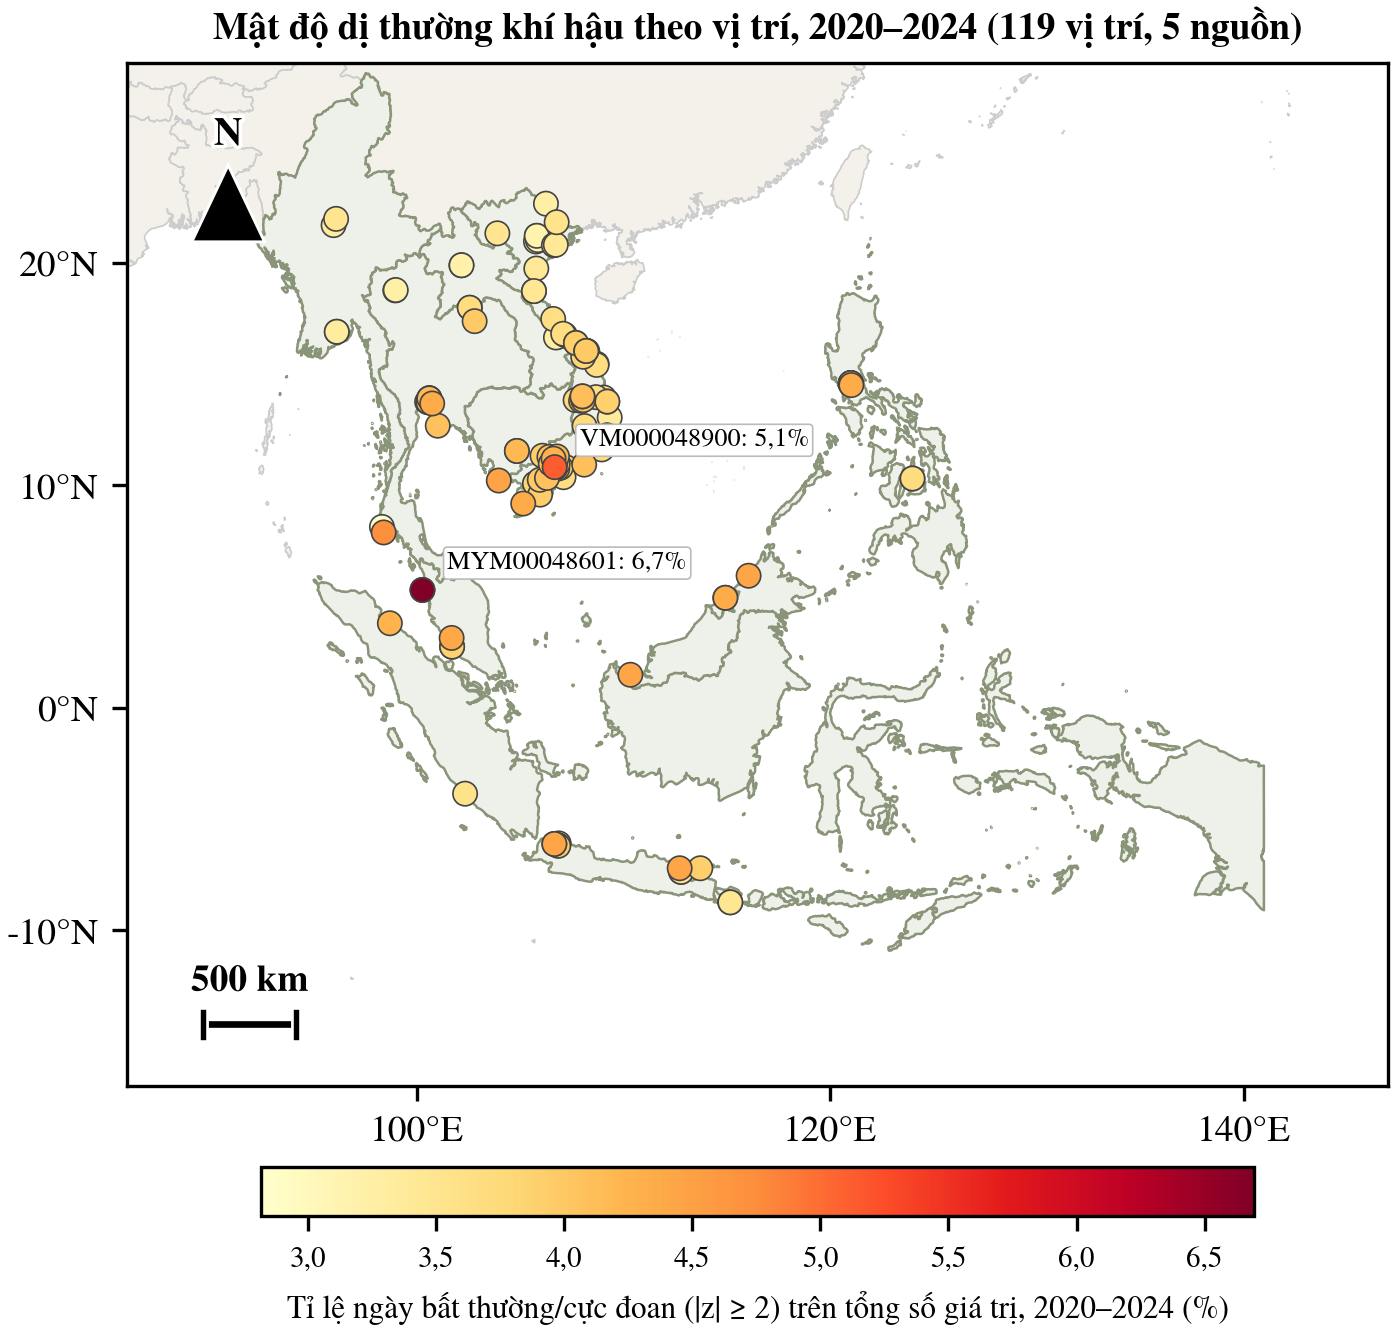
\includegraphics[width=0.78\linewidth]{figures/anomaly_spatial_density.png}
\caption[Mật độ dị thường khí hậu theo vị trí, 2020--2024]{Tỉ lệ ngày bất thường/cực đoan tại 119 vị trí, 2020--2024 (số giá trị bị gắn cờ chia tổng số giá trị có khí hậu nền, gộp \texttt{temp\_mean} và \texttt{pmsl\_min}, mọi nguồn). Ranh giới: Natural Earth 10m, WGS84.}
\label{fig:anomaly-spatial}
\end{figure}

Theo tháng (Hình~\ref{fig:anomaly-time}), tháng nhiều ca nhất là 9/2024 với 880 ca, trong đó 528 ca áp suất do
bão Yagi. Tháng 4/2024 có 371 ca nhiệt độ, 98,4\% lệch dương, nhiều nhất kể từ 2/2023. Đỉnh nhiệt độ lớn nhất
lại là 1/2021 (652 ca), nhưng 96,6\% là ngày \emph{lạnh} bất thường. Vì vậy số ca theo tháng phải đọc kèm dấu
của $z$: cùng một cột cao có thể là nắng nóng hoặc rét đậm.

\begin{figure}[!htbp]
\centering
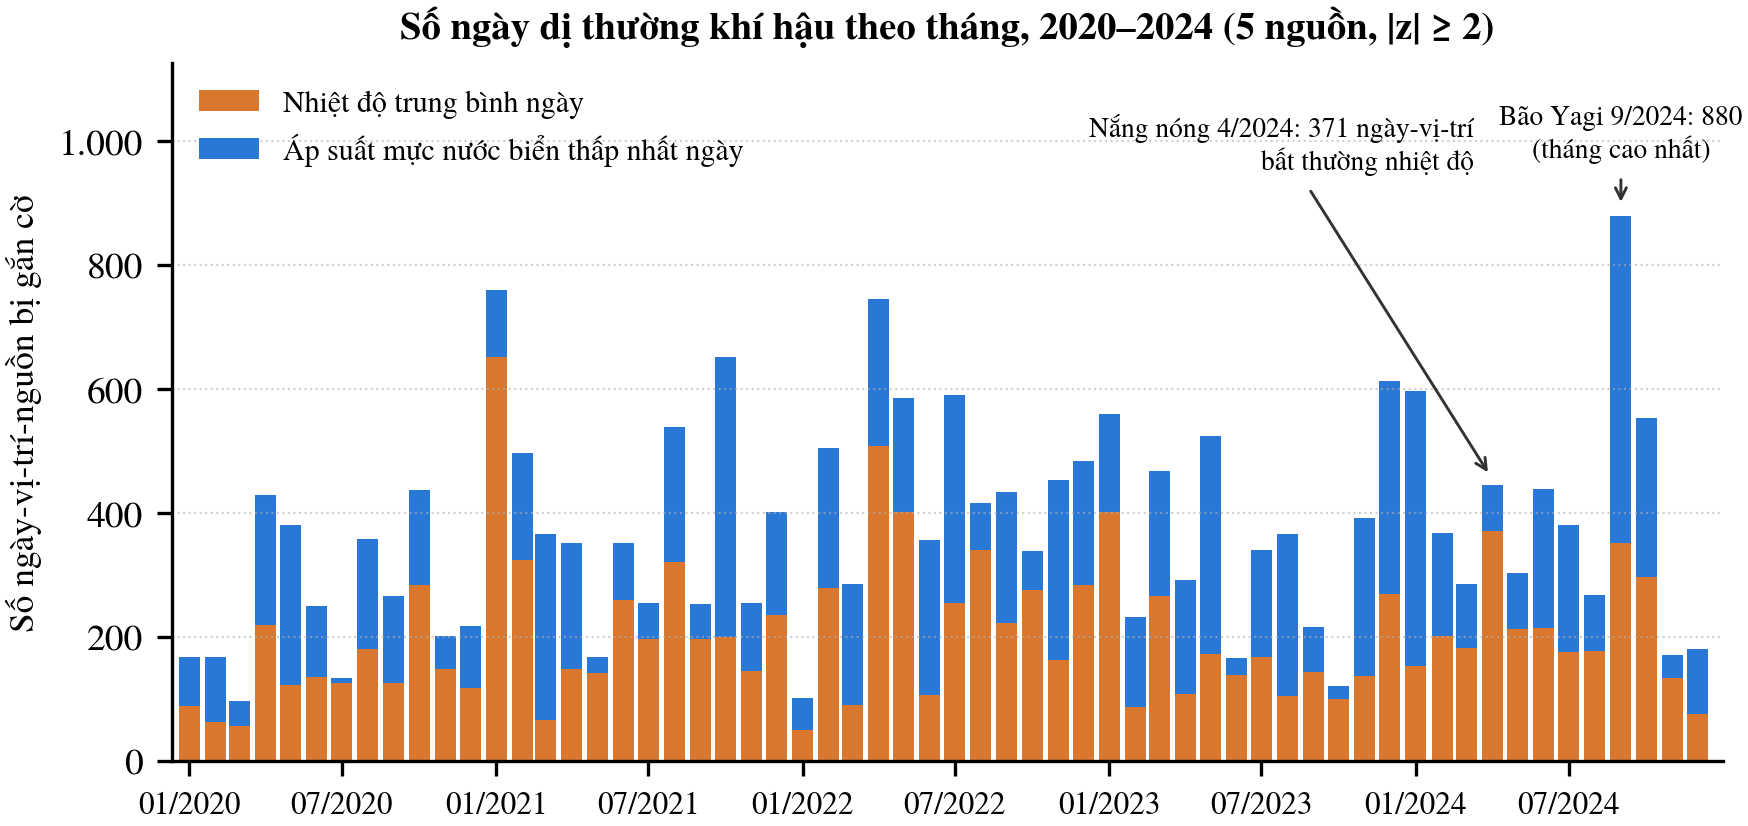
\includegraphics[width=0.9\linewidth]{figures/anomaly_time_distribution.png}
\caption[Số ngày dị thường khí hậu theo tháng, 2020--2024]{Số giá trị ngày bị gắn cờ ($|z|\ge2$) theo tháng, 2020--2024, tách nhiệt độ và áp suất, cả năm nguồn.}
\label{fig:anomaly-time}
\end{figure}

\subsection{Điểm dị thường trong hai sự kiện thật}
\label{sec:anomaly-points}

Hình~\ref{fig:anomaly-event-maps} vẽ từng điểm dị thường trong một ngày của hai sự kiện ở
Bảng~\ref{tab:anomaly-events}. Ngày 30/4/2024, 176/179 giá trị nhiệt độ (98,3\%) lệch dương, 46 giá trị
có $|z|\ge2$ và 4 giá trị có $|z|\ge3$: THW00041018 ($+3{,}53$), MYM00048601 ($+3{,}27$) và trạm WMO 48845
với hai mã GHCN ($+3{,}22$) và ISD ($+3{,}02$); hai mã của cùng một trạm cho cùng kết luận, đúng như Entity
Resolution đã ghép. Ngày 7/9/2024, 11 giá trị áp suất có $z\le-3$, đều ở Bắc Bộ quanh Hải Phòng (978,8~hPa,
$z=-7{,}2$), trong khi Nam Bộ gần như không lệch.

\begin{figure}[!htbp]
\centering
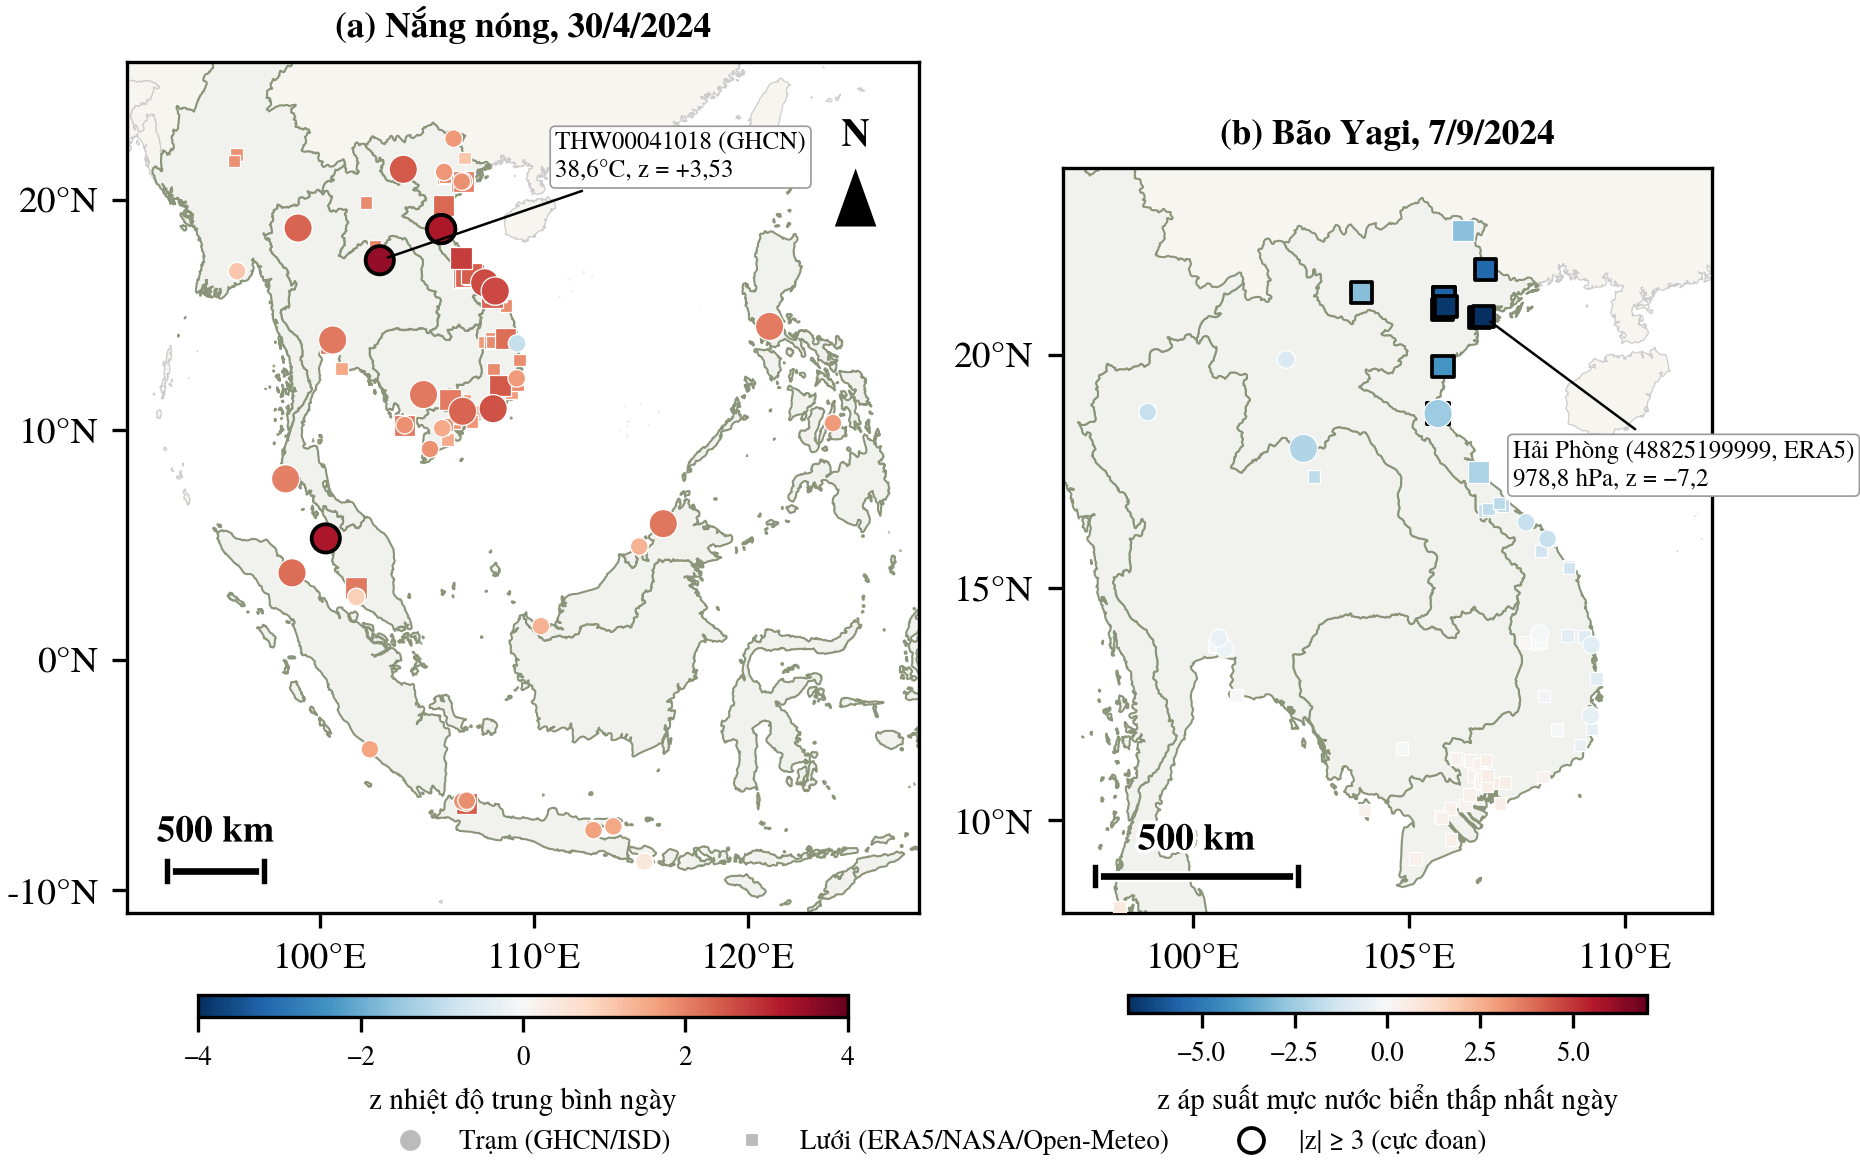
\includegraphics[width=0.9\linewidth]{figures/anomaly_event_maps.png}
\caption[Bản đồ điểm dị thường: nắng nóng 30/4/2024 và bão Yagi 7/9/2024]{Từng điểm dị thường chuẩn hoá $z$ trong một ngày. (a) Nhiệt độ trung bình ngày 30/4/2024, 179 giá trị tại 119 vị trí. (b) Áp suất mực nước biển thấp nhất ngày 7/9/2024, phóng to lục địa. Hình tròn là trạm (GHCN/ISD), hình vuông là lưới (ERA5, NASA POWER, Open-Meteo); viền đen: $|z|\ge3$. Mỗi panel một thang màu đối xứng quanh 0.}
\label{fig:anomaly-event-maps}
\end{figure}

Ở mức một trạm (Hình~\ref{fig:anomaly-station-series}), dị thường là các điểm rơi ra ngoài dải nền $\pm2\sigma$.
Tại Bangkok, nắng nóng 4/2024 chỉ có một ngày vượt ngưỡng (21/4, 33,8\,°C, $z=+2{,}01$); sáu ngày còn lại bị
gắn cờ đều là ngày mát bất thường, mạnh nhất 4/7 (26,1\,°C, $z=-3{,}00$). Nắng nóng ở đây là nhiều tuần sát cận
trên của dải nền, nên cần thêm chỉ số đợt nóng TG90p bên cạnh $z$. Tại Hải Phòng, áp suất rơi từ 992,6~hPa
ngày 6/9 ($z=-3{,}25$) xuống 978,8~hPa ngày 7/9 rồi về lại dải nền sau hai ngày, đúng dạng bão đi qua.

\begin{figure}[!htbp]
\centering
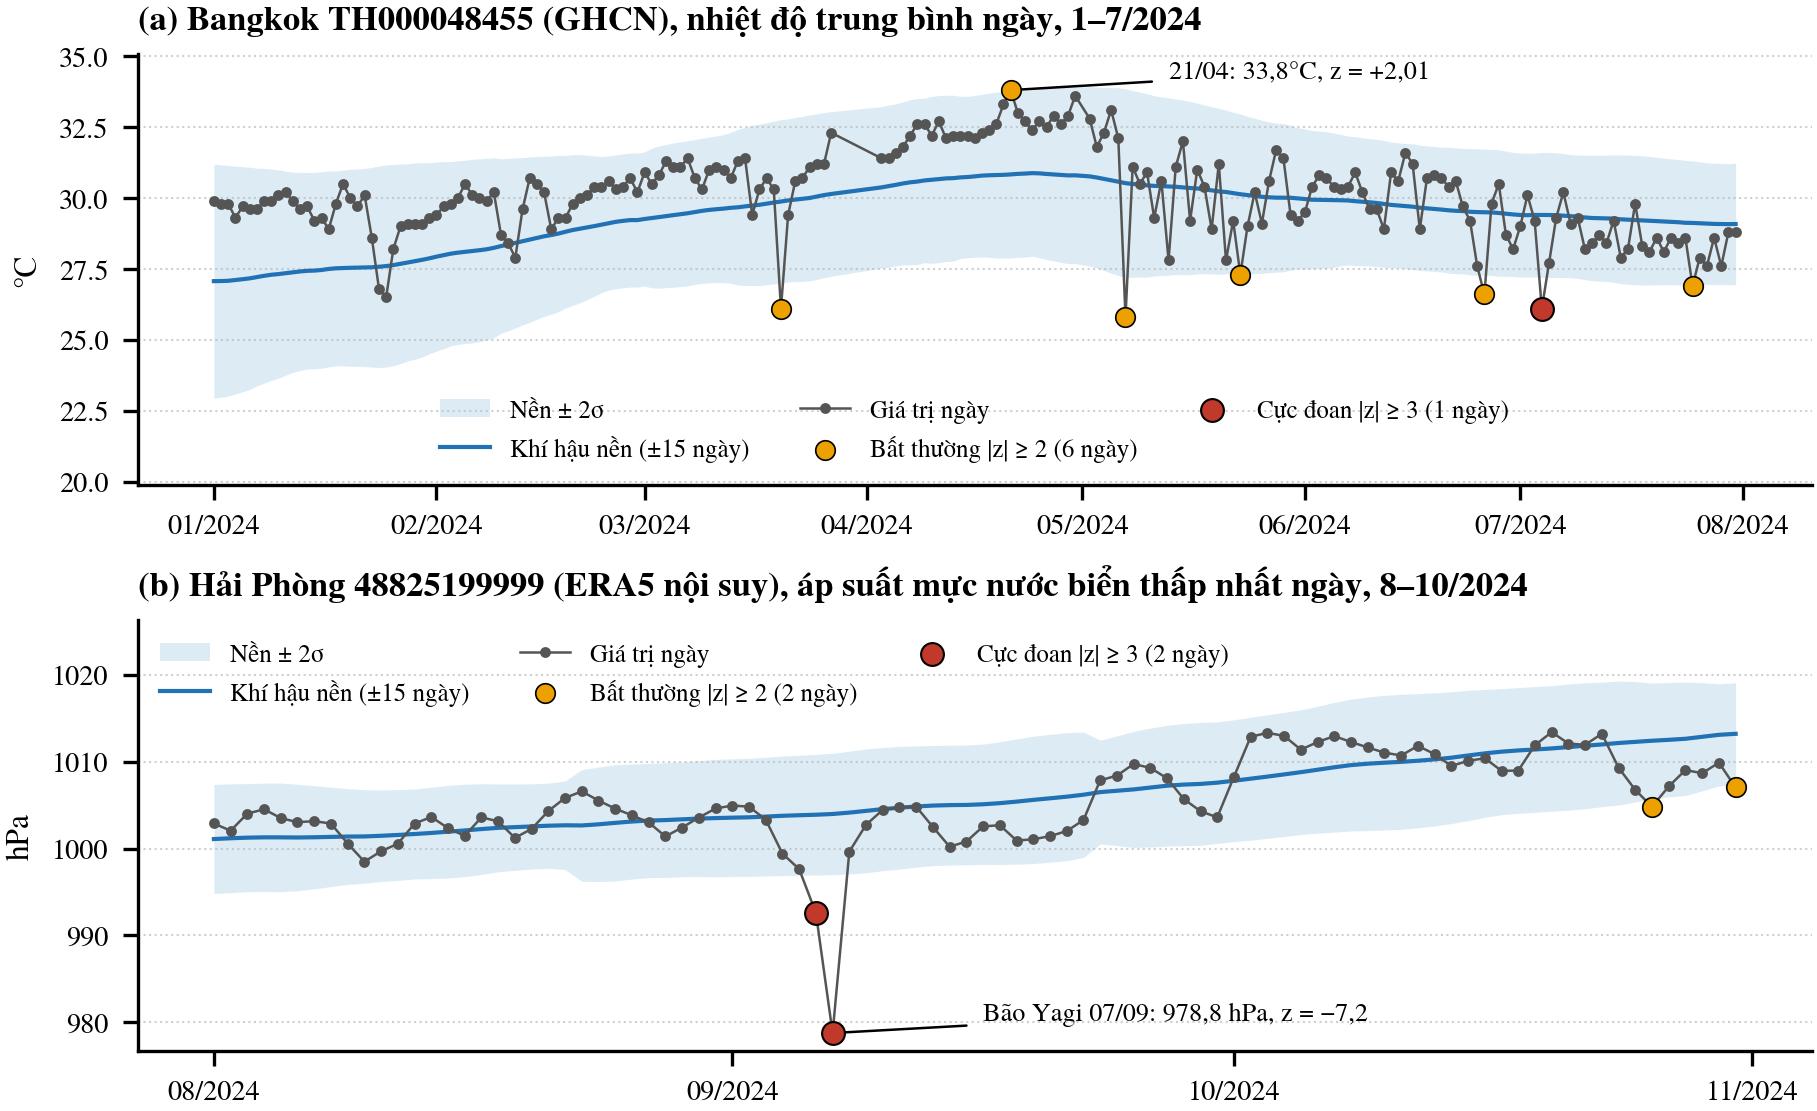
\includegraphics[width=0.9\linewidth]{figures/anomaly_station_timeseries.png}
\caption[Chuỗi ngày tại trạm kèm các điểm dị thường]{(a) Bangkok TH000048455 (GHCN), nhiệt độ trung bình ngày 1--7/2024. (b) Hải Phòng 48825199999 (ERA5 nội suy), áp suất mực nước biển thấp nhất ngày 8--10/2024. Đường xanh: khí hậu nền $\pm15$ ngày; dải nhạt: nền $\pm2\sigma$; điểm cam: bất thường; điểm đỏ: cực đoan.}
\label{fig:anomaly-station-series}
\end{figure}

\subsection{Đợt nóng, hạn và mưa cực đoan}
\label{sec:heat-drought-rain}

Trong 2020--2024 có 3.832 đợt nóng bắt đầu (ERA5 2.064; GHCN 1.134; ISD 423; Open-Meteo 107; NASA POWER 104).
Phân bố độ dài lệch phải (Hình~\ref{fig:heatwave-duration}): trung vị 4 ngày, 68,6\% số đợt chỉ 3--4 ngày, 116
đợt từ 10 ngày trở lên. Hai đợt dài nhất cùng ở Phuket (TH000048564): 43 ngày từ 26/1/2024 và 30 ngày từ
3/4/2024; tiếp theo là Jakarta, 29 ngày từ 25/9/2023 (IDM00096749), và Tân Sơn Nhất, 27 ngày từ 7/4/2024. Các
đợt dài dồn vào cuối 2023 và nửa đầu 2024, khớp với đợt nắng nóng ở Bảng~\ref{tab:anomaly-events}.

\begin{figure}[!htbp]
\centering
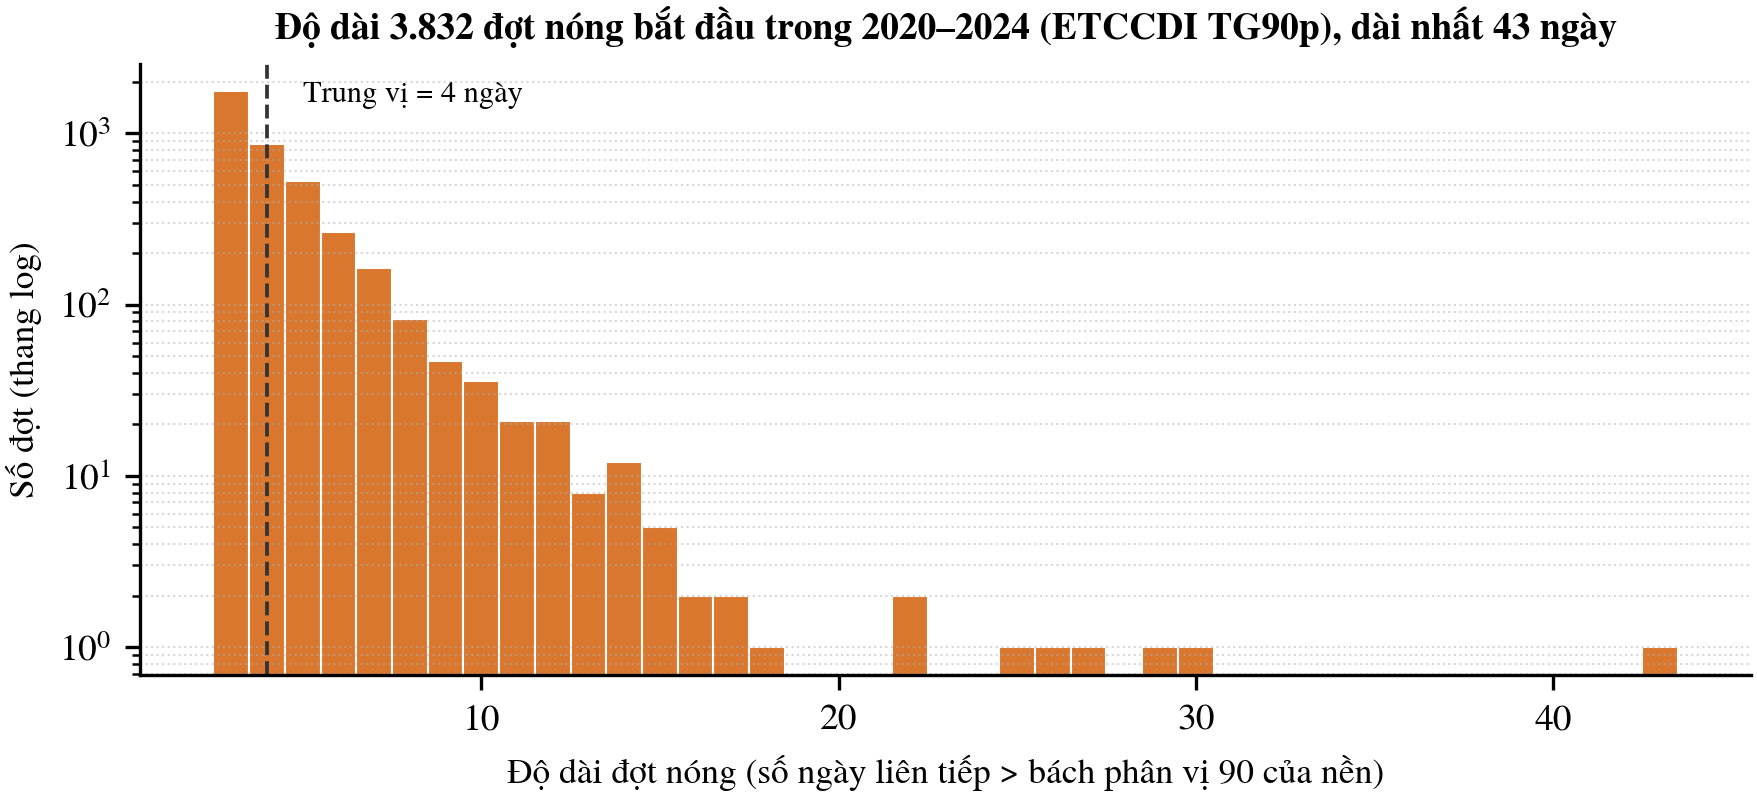
\includegraphics[width=0.82\linewidth]{figures/heatwave_duration_hist.png}
\caption[Phân bố độ dài các đợt nóng, 2020--2024]{Độ dài 3.832 đợt nóng bắt đầu trong 2020--2024 (ETCCDI TG90p), trục tung thang log.}
\label{fig:heatwave-duration}
\end{figure}

Hình~\ref{fig:spi3-mekong} cho SPI-3 của hai trạm duy nhất trong vùng Mekong đủ chuỗi mưa tháng, Cà Mau và
Phan Thiết (71 tháng--trạm trong 2020--2024). Chỉ đuôi 1--5/2020 của đợt hạn 2019--2020 nằm trong cửa sổ, và
4/7 tháng--trạm của đoạn này có SPI-3 $\le-1$, so với 9,9\% của cả 2020--2024; cả giai đoạn không tháng nào
xuống dưới $-1{,}5$. Hệ thống bắt được đúng chiều tín hiệu hạn, nhưng hai trạm ven biển với nhiều tháng thiếu
số liệu chưa đủ đại diện cho cả lưu vực.

\begin{figure}[!htbp]
\centering
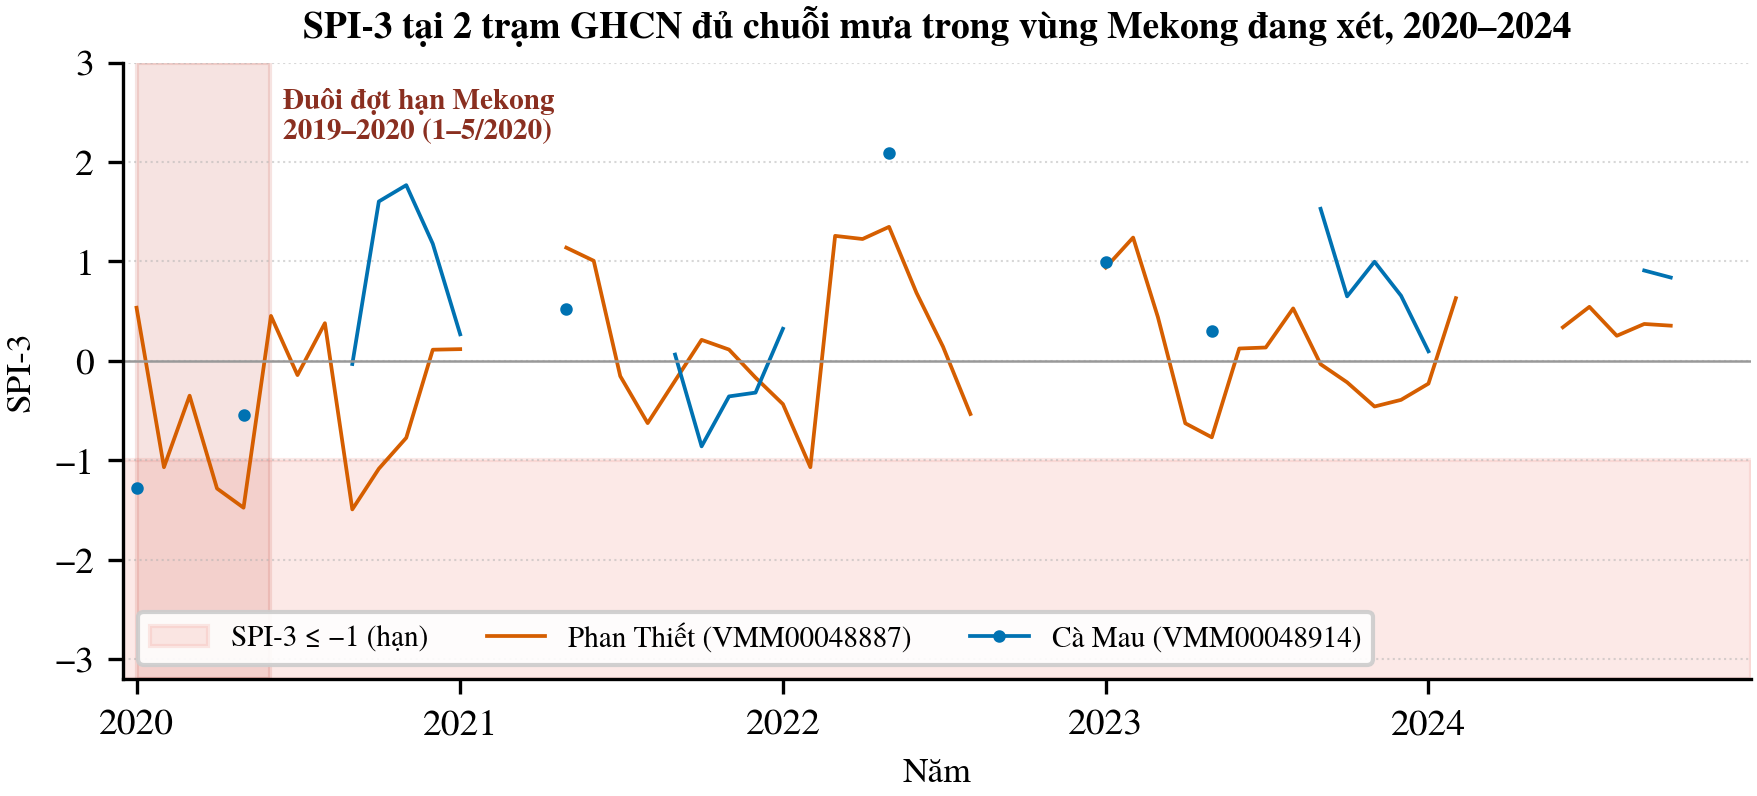
\includegraphics[width=0.82\linewidth]{figures/spi3_mekong_timeseries.png}
\caption[SPI-3 tại hai trạm vùng Mekong, 2020--2024]{SPI-3 (nền GHCN 1991--2020) tại Cà Mau (VMM00048914) và Phan Thiết (VMM00048887), 2020--2024. Đường ngắt ở khoảng trống trên 3 tháng (tháng thiếu trên 10\% số ngày bị loại). Vùng đỏ dọc: 1--5/2020, phần đuôi của đợt hạn Mekong 6/2019--5/2020 nằm trong cửa sổ.}
\label{fig:spi3-mekong}
\end{figure}

Về mưa (Hình~\ref{fig:r95ptot-country}), trong 2020--2024 khoảng một phần năm đến một phần tư lượng mưa năm
rơi vào những ngày vượt bách phân vị 95: cao nhất Philippines (27,6\%, 40 năm--vị trí) và Việt Nam (24,6\%,
371), thấp nhất Campuchia (19,2\%, 10). Chênh lệch chỉ khoảng 8 điểm phần trăm và nhiều nước có ít
năm--vị trí, nên không nên xếp hạng chặt giữa các nước.

\begin{figure}[!htbp]
\centering
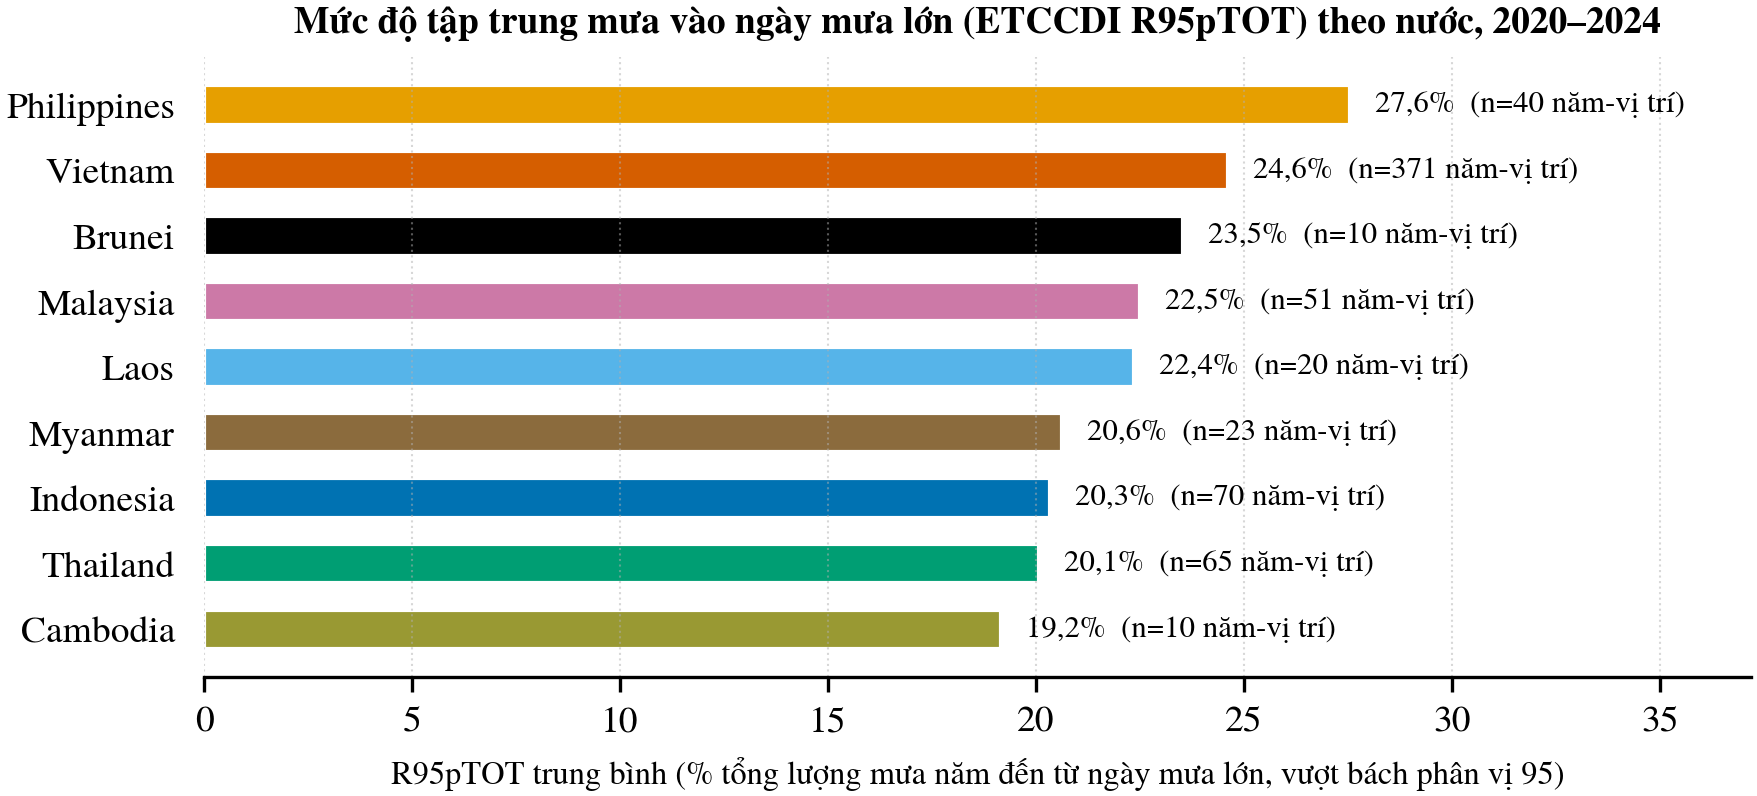
\includegraphics[width=0.82\linewidth]{figures/precip_r95ptot_by_country.png}
\caption[Chỉ số mưa cực đoan R95pTOT theo nước, 2020--2024]{R95pTOT trung bình theo nước, 2020--2024 (năm có từ 90\% số ngày có số liệu mưa, nước có từ 3 năm--vị trí; mỗi nguồn tại cùng vị trí tính riêng).}
\label{fig:r95ptot-country}
\end{figure}

\subsection{Xác nhận chéo đa nguồn}
\label{sec:anomaly-crosscheck}

Bước gắn trực tiếp với tích hợp dữ liệu là \emph{xác nhận chéo}: mỗi dị thường tại trạm GHCN/ISD được đối
chiếu với ERA5 nội suy đúng \texttt{location\_id} và với các trạm khác trong bán kính 200~km (bỏ các cặp dưới
5~km, vốn là cùng một trạm vật lý theo Entity Resolution). Dị thường được xác nhận là khí hậu thật khi ERA5
lệch cùng chiều ($|z|\ge1$) hoặc ít nhất một nửa trạm lân cận đồng chiều; bị coi là nghi lỗi khi trạm ở mức
cực đoan mà mọi đối chứng đều không ủng hộ.

Trong 2020--2024 (Hình~\ref{fig:anomaly-confirmation}), 5.515/5.910 ca (93,3\%) được xác nhận, 375 ca (6,3\%)
là dị thường cục bộ, 20 ca (0,3\%) nghi lỗi, và không ca nào thiếu đối chứng. So với chỉ dùng ERA5, trạm lân
cận thêm 135 ca được xác nhận, trong đó 3 ca từng bị nghi lỗi. Ví dụ: ISD Phnom Penh ngày 3/7/2023 có áp suất
thấp nhất $z=-5{,}5$ trong khi ERA5 cùng vị trí bình thường ($z=+1{,}6$); 13/20 ca nghi lỗi của cả cửa sổ thuộc
trạm này, dày đặc 6--9/2023, khớp với trôi áp suất ở Mục~6.10. Một nguồn đơn lẻ không tự phân biệt được cực
đoan thật với cảm biến hỏng; tích hợp trạm với lưới tái phân tích thì tách được.

\begin{figure}[!htbp]
\centering
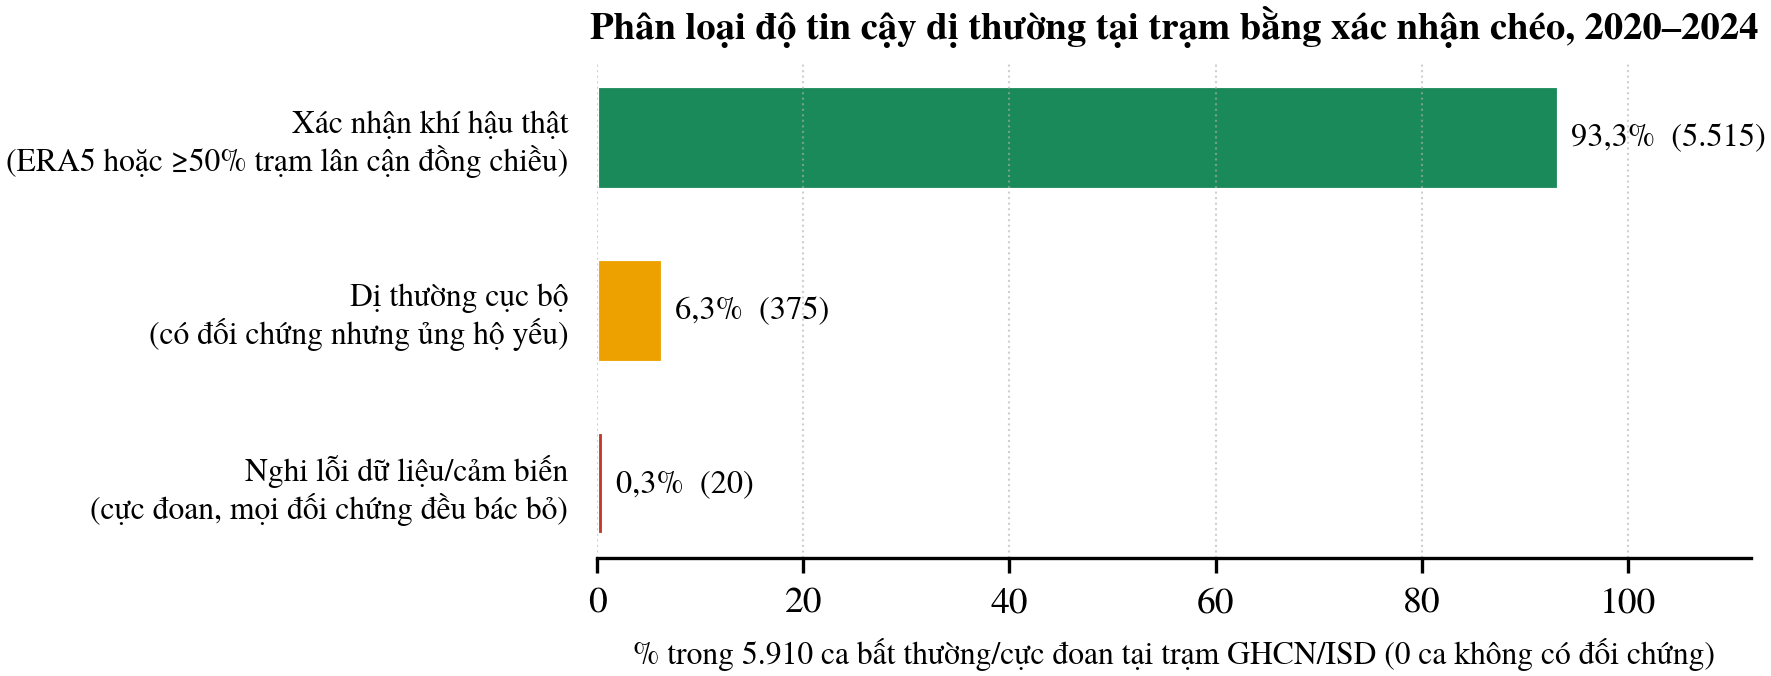
\includegraphics[width=0.84\linewidth]{figures/anomaly_confirmation_breakdown.png}
\caption[Phân loại độ tin cậy của dị thường tại trạm, 2020--2024]{Phân loại 5.910 ca bất thường/cực đoan tại trạm GHCN/ISD, 2020--2024, theo hai đối chứng độc lập: ERA5 nội suy cùng vị trí, cùng ngày và các trạm lân cận trong bán kính 200~km (\texttt{classify\_combined()} trong \path{warehouse/anomaly_detection.py}). Không có ca nào thiếu đối chứng.}
\label{fig:anomaly-confirmation}
\end{figure}

\section{Xu hướng khí hậu dài hạn}

Để tách biến đổi dài hạn khỏi dị thường ngắn hạn, \path{warehouse/climate_trends.py} áp dụng kiểm định
Mann--Kendall~\cite{mann1945nonparametric,kendall1975rank} (có hiệu chỉnh nhóm giá trị trùng) và độ dốc
Sen~\cite{sen1968estimates} trên chuỗi nhiệt độ trung bình năm của trạm GHCN; cả hai phi tham số và bền
với ngoại lai. Năm hợp lệ cần ít nhất 80\% số ngày có số liệu, mỗi chuỗi cần ít nhất 30 năm. Giai đoạn
1975--2024 có \textbf{25/27 trạm ấm lên có ý nghĩa} ($p < 0{,}05$), độ dốc Sen trung vị
\textbf{+0,21\textdegree{}C/thập kỷ}; nhanh nhất là Jakarta (+0,41), Penang (+0,35), Bangkok (+0,35) và Cao
Bằng (+0,34). Mưa chỉ có 1 đến 6 trạm đủ 30 năm nên chưa kết luận. Hạn chế: chưa hiệu chỉnh tự tương quan
Hamed--Rao~\cite{hamed1998modified}, và trạm đổi cách tính nhiệt độ ngày có thể tạo xu hướng giả (Mục~6.10).

\section{Phát hiện trôi cảm biến}

\path{warehouse/sensor_drift.py} đồng nhất hoá chuỗi (homogenization) bằng chuỗi tham chiếu: với mỗi
trạm, lấy chênh lệch trung bình tháng giữa trạm và ERA5 nội suy cùng vị trí, cùng ngày, nên biến động
khí hậu thật bị triệt tiêu và phần còn lại phản ánh lỗi cảm biến hoặc điểm đo. Trôi dần được kiểm định
bằng Mann--Kendall và độ dốc Sen, nhảy bậc bằng kiểm định Pettitt~\cite{pettitt1979nonparametric}. Chuỗi
chỉ bị gắn cờ khi vừa có ý nghĩa ($p < 0{,}05$) vừa vượt ngưỡng vật lý (nhiệt độ 0,3\textdegree{}C/năm
hoặc bước 0,5\textdegree{}C; áp suất 0,5~hPa/năm hoặc bước 1~hPa).

Trên 80 chuỗi trạm--biến (2020--2024), hệ thống gắn cờ 4 chuỗi (Hình~\ref{fig:data-error-density}b).
Rõ nhất là áp suất ISD Phnom Penh: trôi $-0{,}65$~hPa/năm, điểm gãy 11/2022, bước $-2{,}6$~hPa, khớp với
ca nghi lỗi phát hiện độc lập ở Mục~6.8. Ba chuỗi nhiệt độ (Viêng Chăn, Cần Thơ, một trạm GHCN ở Thái
Lan) nhảy bậc $-0{,}5$ đến $-0{,}7$\textdegree{}C quanh 2021--2022, nhiều khả năng do thay thiết bị hoặc
dời điểm đo. Tiêm trôi và bước nhảy nhân tạo (gấp đôi ngưỡng) vào 76 chuỗi ổn định cho tỷ lệ phát hiện
100\% với trôi và 95--98\% với nhảy bậc.

\section{Phân tích khám phá dữ liệu (EDA) và thành phần chính (PCA)}
\label{sec:eda-pca}

Trước khi tin ngưỡng hay mô hình nào, \texttt{warehouse/eda\_pca.py} kiểm tra phân phối và tương quan
trên kho đầy đủ (8.955.313 dòng). Lượng mưa và bức xạ lệch phải rất mạnh trên mọi nguồn (đa số gần 0,
đuôi dài do mưa cực đoan), là cơ sở định lượng để dùng IQR thay Z-score (Mục~6.12) và ngưỡng bách phân
vị ETCCDI/SPI thay $z$-score cho mưa (Mục~6.8). Tương quan Pearson ở Bảng~\ref{tab:correlation} tính
theo từng cặp biến trên các dòng đủ hai giá trị, không điền 0 vào chỗ thiếu (cách làm từng tạo tương
quan giả gió--độ ẩm $+0{,}57$, Mục~6.12); hệ số nhiệt độ--độ ẩm của ISD ($-0{,}59$) khớp với lần tính
độc lập ở Mục~6.12.

\begin{table}[H]
\centering\small
\caption{Tương quan Pearson giữa các biến, tính pairwise-complete trên dữ liệu thật}
\label{tab:correlation}
\begin{tabular}{@{}lrl@{}}
\toprule
\textbf{Nguồn} & \textbf{Cặp biến} & \textbf{Hệ số} \\
\midrule
Open-Meteo (263.088 dòng) & Nhiệt độ $\leftrightarrow$ Độ ẩm & $-0{,}52$ \\
Open-Meteo & Nhiệt độ $\leftrightarrow$ Áp suất MSL & $-0{,}56$ \\
Open-Meteo & Độ ẩm $\leftrightarrow$ Tốc độ gió & $-0{,}34$ \\
ISD (2.529.497 dòng đủ 4 biến) & Nhiệt độ $\leftrightarrow$ Độ ẩm & $-0{,}59$ \\
ISD & Nhiệt độ $\leftrightarrow$ Điểm sương & $+0{,}45$ \\
ISD & Độ ẩm $\leftrightarrow$ Điểm sương & $+0{,}43$ \\
\bottomrule
\end{tabular}
\end{table}

PCA cho biết 5--6 biến đo cùng lúc có bao nhiêu trục biến động độc lập (Bảng~\ref{tab:pca}). Dữ liệu
được chuẩn hoá Z-score, hướng gió tách thành $\sin$/$\cos$ để $359°$ và $1°$ gần nhau đúng như vật lý.
PC2 của Open-Meteo (ẩm, mưa và áp thấp cùng biến thiên) tự hiện ra mà không cần gán nhãn, đúng chữ ký
thống kê của bão/áp thấp nhiệt đới mà hệ thống dùng để bắt bão Yagi (Mục~6.8). PC1+PC2 chỉ giải thích
48--56\% phương sai: khí tượng Đông Nam Á có nhiều hơn hai trục biến động độc lập, đúng kỳ vọng vật lý
chứ không phải dấu hiệu PCA thất bại.

\begin{table}[H]
\centering\small
\caption{Kết quả PCA: tỷ lệ phương sai giải thích và diễn giải vật lý của hai thành phần đầu}
\label{tab:pca}
\begin{tabular}{@{}lrrp{3.3cm}p{3.3cm}@{}}
\toprule
\textbf{Nguồn} & \textbf{PC1} & \textbf{PC1+PC2} & \textbf{PC1 (hệ số tải lớn)} & \textbf{PC2} \\
\midrule
Open-Meteo & 27,2\% & 48,2\% & Nóng + áp thấp + gió mạnh & Ẩm + mưa + áp thấp \\
ISD & 29,9\% & 56,1\% & Nóng + khô + gió mạnh & Điểm sương cao (ẩm tuyệt đối) \\
\bottomrule
\end{tabular}
\end{table}

\section{Đánh giá chất lượng dữ liệu}

Trong thí nghiệm có đối chứng (tiêm 5 giá trị cực đoan vào dữ liệu mô phỏng), Z-score chỉ bắt được 1/5
vì chính các giá trị cực đoan làm độ lệch chuẩn phình từ 2,0 lên 72,2 (\textit{masking effect}), còn
IQR dựa trên tứ phân vị bắt đủ 5/5. Vì vậy IQR là chỉ số chính của báo cáo chất lượng tự động
(\texttt{archived/docs/13-data-quality-report.md}). Chạy lại trên bộ đầy đủ còn lộ bốn lỗi của pipeline, đã sửa:
(i) gió Open-Meteo theo km/h bị ghi thẳng vào \texttt{wind\_speed\_ms} (phóng đại 3,6 lần), nay đọc đơn
vị từ \texttt{hourly\_units}; (ii) tương quan tính sau khi điền 0 tạo tương quan giả, tính lại theo cặp
cho nhiệt độ--độ ẩm $-0{,}59$ và nhiệt độ--áp suất $-0{,}61$; (iii) phép đo partition so với bản sao cũ;
(iv) ERA5 bị ánh xạ bức xạ đỉnh khí quyển thay vì bức xạ bề mặt.

Bốn tầng QC ở Ingestion (\texttt{archived/docs/17}) đặt rỗng giá trị lỗi và ghi lý do vào cột \texttt{qc\_flag},
không xoá dòng (Hình~\ref{fig:qc-flags}). Tầng 1 đọc cờ QC của NOAA: trước đó pipeline vẫn dùng 406 giá
trị GHCN và 3.255 giá trị ISD bị NOAA đánh dấu sai, kể cả hai bản tin gió 83~m/s. Tầng 2 kiểm tra giới
hạn vật lý, tầng 3--4 kiểm tra nhất quán nội bộ và bước nhảy phi vật lý (18 điểm nhiệt độ, 18 điểm áp
suất). Ngoài ra, nhóm gộp 393.155 bản tin ISD trùng (METAR và SYNOP), đọc áp suất trạm ISD vào cột áp
suất bề mặt, tải gió NASA POWER ở 10~m thay vì 2~m, và sửa lỗi bỏ trống ngày thiếu TAVG dù đủ TMAX/TMIN
(tỷ lệ thiếu nhiệt độ GHCN giảm từ 4,1\% xuống 0,3\%). Các kết luận chính không đổi sau khi làm sạch.

\begin{figure}[H]
\centering
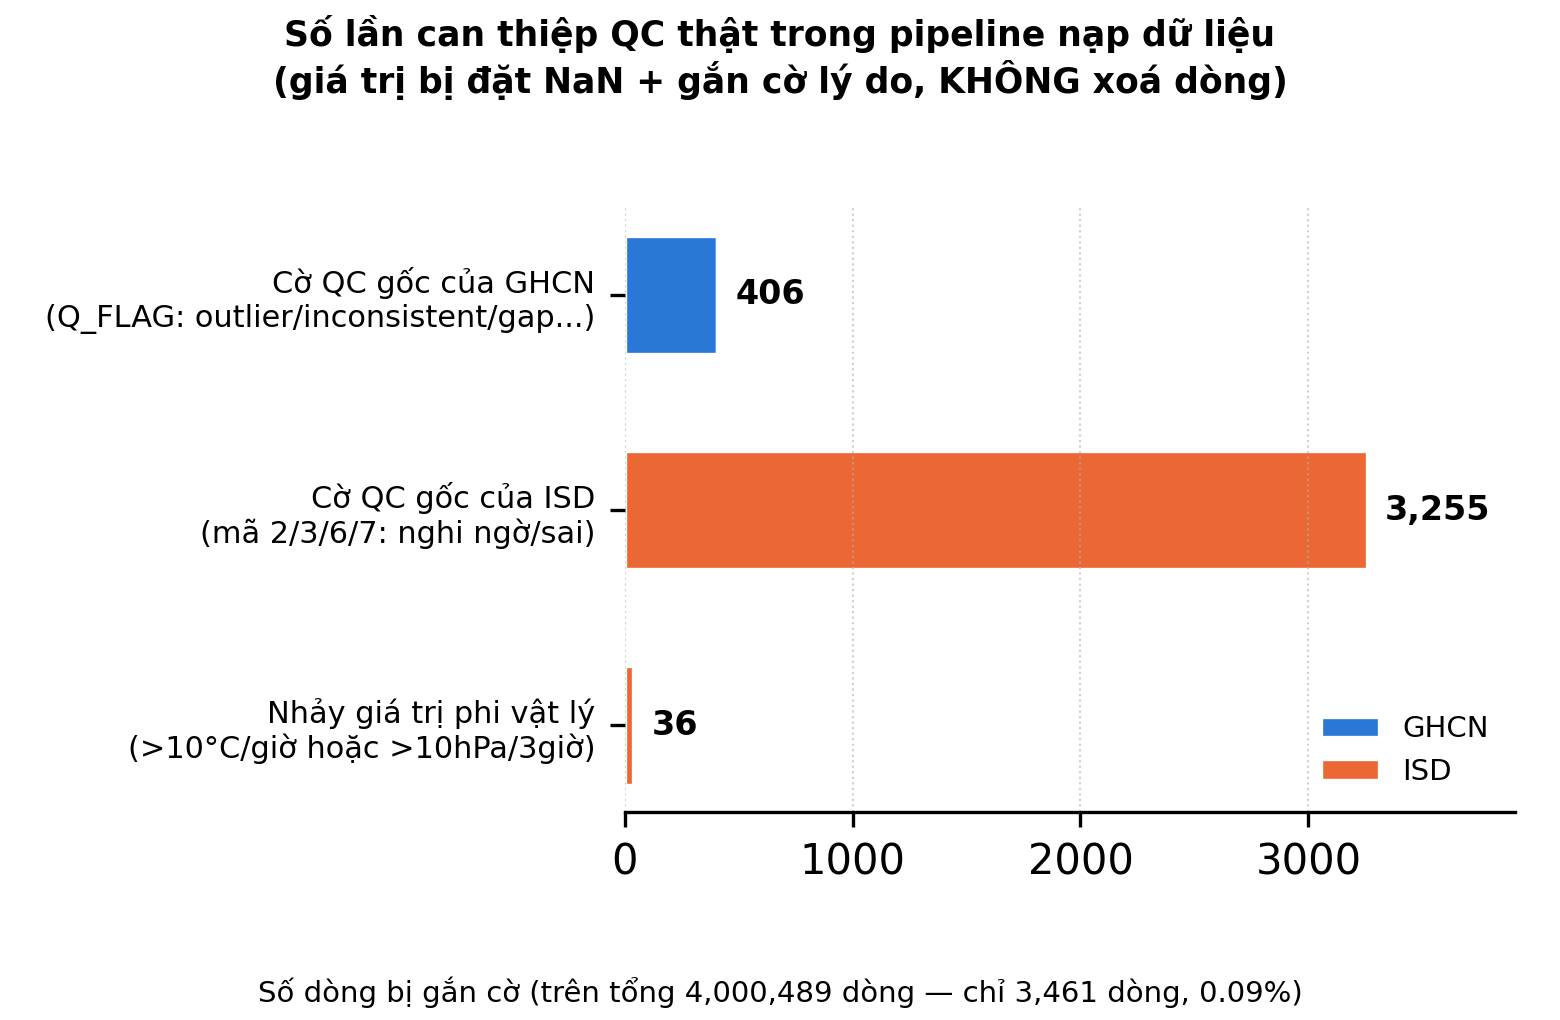
\includegraphics[max width=\linewidth]{figures/data_quality_qc_flags.png}
\caption[Số lần can thiệp QC theo loại cờ]{Số lần can thiệp QC theo loại cờ (406 GHCN, 3.255 ISD,
36 bước nhảy = 18+18), chiếm 0,09\% tổng số dòng.}
\label{fig:qc-flags}
\end{figure}

Hình~\ref{fig:data-error-density} đưa lỗi về từng trạm trong cửa sổ 2020--2024. Ở tầng Ingestion,
1.590 dòng có cờ QC nằm ở 32/61 trạm GHCN/ISD (ISD 1.561, GHCN 29), nhưng năm trạm ISD ở Campuchia, Lào,
Myanmar và Thái Lan chiếm 56,4\%, tức lỗi gắn với trạm và cơ quan vận hành. Ở tầng phân tích chỉ còn 20
ca nghi lỗi ở 8 trạm vì giai đoạn này luôn có ERA5 để đối chiếu; riêng ISD Phnom Penh chiếm 13 ca (65\%).
Hai tầng bổ sung nhau: cờ NOAA bắt giá trị sai trong từng bản tin, xác nhận chéo bắt chuỗi lệch so với
ERA5 và trạm lân cận. Phnom Penh (1) có mặt ở cả ba lớp (219 dòng gắn cờ QC, 13 ca nghi lỗi, trôi áp
suất), Viêng Chăn (3) ở hai lớp (210 dòng, nhảy bậc nhiệt độ); đây là các trạm cần kiểm tra hồ sơ thiết
bị trước khi dùng chuỗi.

\begin{figure}[H]
\centering
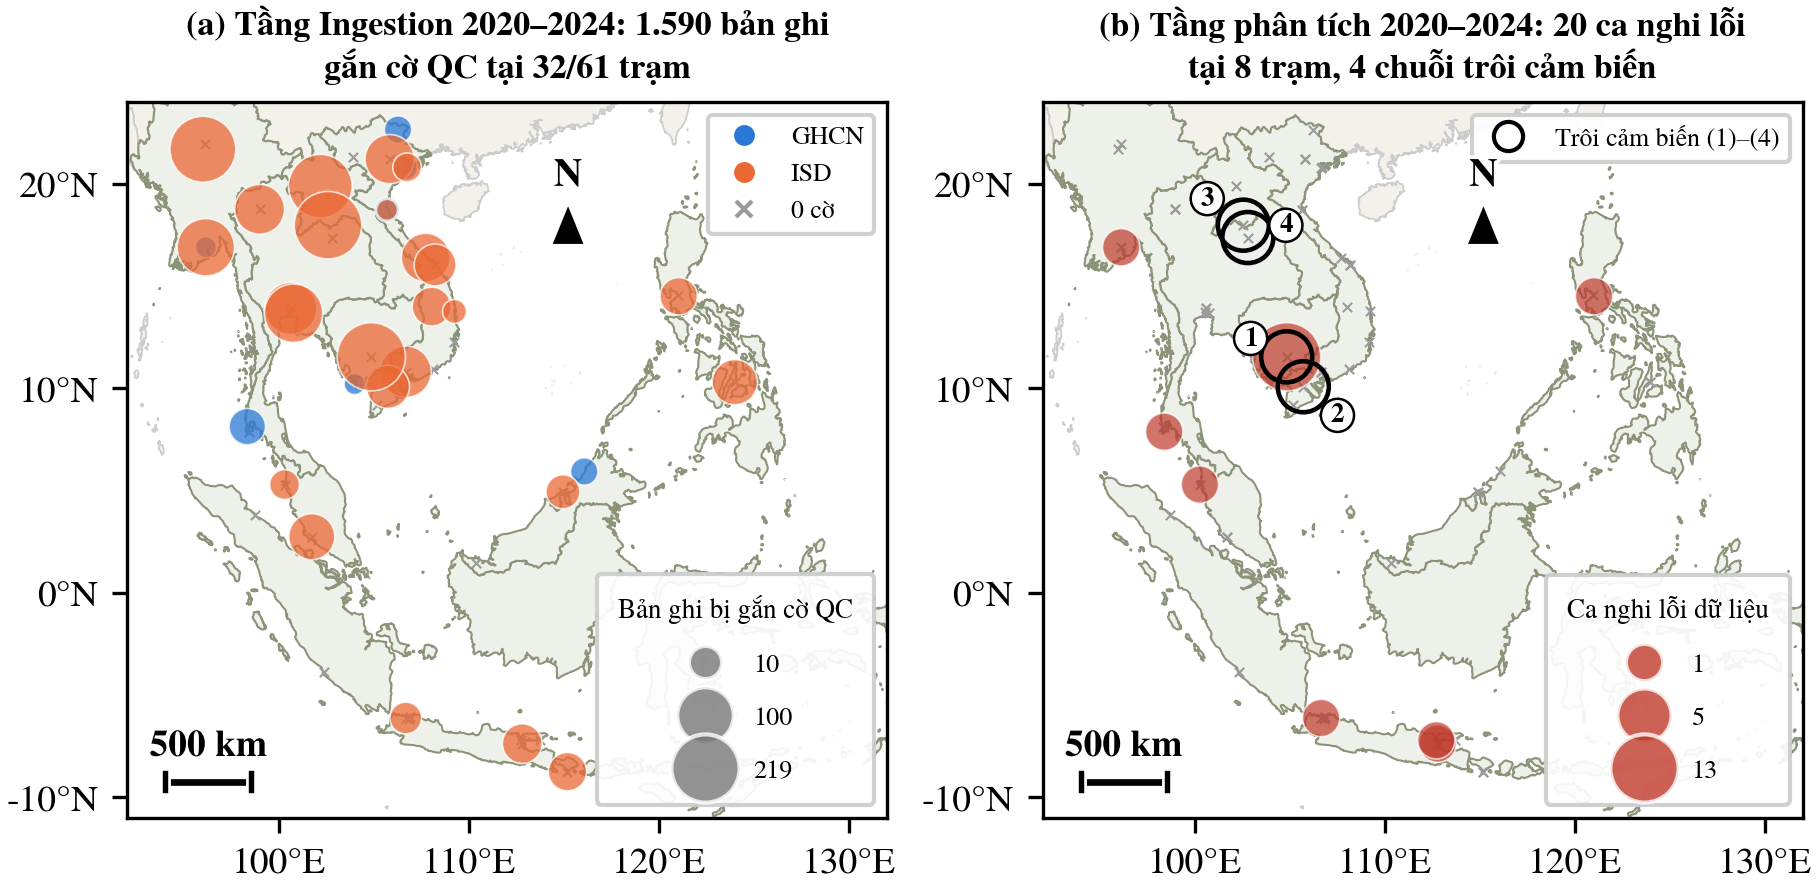
\includegraphics[max width=\linewidth]{figures/data_error_density.png}
\caption[Mật độ trạm đo lỗi dữ liệu 2020--2024 theo hai tầng phát hiện]{Mật độ lỗi dữ liệu 2020--2024
tại 61 trạm GHCN/ISD (diện tích bong bóng tỉ lệ thuận với số lỗi; $\times$: trạm không có lỗi). (a) Số
dòng có ít nhất một cờ QC, tô theo nguồn; một dòng có thể mang nhiều cờ và Hình~\ref{fig:qc-flags} đếm
trên toàn chuỗi nên hai con số khác nhau. (b) Số ca \texttt{nghi\_loi\_du\_lieu} từ xác nhận chéo; vòng
đen là chuỗi trôi cảm biến: (1) Phnom Penh, ISD, trôi áp suất $-0{,}65$~hPa/năm, bước $-2{,}6$~hPa từ
11/2022; (2) Cần Thơ, ISD, nhảy bậc nhiệt độ $-0{,}52$°C từ 11/2021; (3) Viêng Chăn, ISD, $-0{,}56$°C từ
3/2022; (4) GHCN THW00041018, Thái Lan, $-0{,}69$°C từ 5/2022. Ranh giới: Natural Earth 10m, EPSG:4326.}
\label{fig:data-error-density}
\end{figure}

\section{Tiến độ tổng thể tại thời điểm báo cáo}

Tiến độ được quản lý theo kế hoạch tuần, mỗi hạng mục có tiêu chí hoàn thành (Definition of Done) đối
chiếu với bằng chứng. Tại thời điểm báo cáo, mọi hạng mục kỹ thuật bắt buộc đã xong và có bằng chứng ở
Chương~6: đủ năm nguồn đúng phạm vi đề cương, Spark batch và streaming chạy thật, dị thường đối chứng
được với sự kiện thật, dashboard kiểm tra qua trình duyệt. Việc còn lại là phối hợp ở tuần cuối (diễn
tập, phân công trình bày).

% ==========================================================
\chapter{Đóng góp dự kiến}
% ==========================================================

\section{Đóng góp về sản phẩm}

Sản phẩm chính là một kho dữ liệu khí tượng đã chuẩn hoá cho Đông Nam Á, dùng lại được cho nhiều bài
toán phân tích. Trên kho này, nhóm đã cài đặt phát hiện dị thường khí hậu và đối chứng với ba sự kiện
thật (Mục~6.8--6.10). Thống kê hỗ trợ nông nghiệp/năng lượng tái tạo và khuyến nghị khung giờ bay UAV
là hai ứng dụng kho đủ khả năng phục vụ nhưng chưa cài đặt (Mục~\ref{sec:future-work}).

\section{Đóng góp về phương pháp}
\label{sec:contributions}

Đề tài không đề xuất kỹ thuật lý thuyết mới mà kiểm chứng có hệ thống các kỹ thuật tích hợp dữ liệu
lớn (Chương~2) trên một miền dị biệt không-thời gian rõ hơn các ví dụ bảng quan hệ thường gặp. Số liệu
thực nghiệm cho thấy: (i) mediated schema GAV đơn giản xử lý được năm nguồn với ba dạng cú pháp khác
nhau nhờ bước PIVOT/PARSE tường minh; (ii) tách \texttt{pressure\_surface\_hpa} và
\texttt{pressure\_msl\_hpa} ngay từ thiết kế lược đồ (Mục~3.2) tránh gộp nhầm hai đại lượng vật lý;
(iii) Survivorship theo xếp hạng độ tin cậy nguồn (Mục~3.3) xử lý đúng xung đột giá trị thay vì lấy
trung bình. Riêng PINN chưa vượt baseline hồi quy thuần ở quy mô hiện tại (Mục~6.5), nên đây là câu
hỏi mở chứ chưa phải đóng góp đã khẳng định.

% ==========================================================
\chapter{Quản lý rủi ro}
% ==========================================================

Bảng~\ref{tab:risks} tổng hợp các rủi ro chính và phương án dự phòng cụ thể.

\begin{table}[H]
\centering\small
\caption{Rủi ro và phương án dự phòng}
\label{tab:risks}
\begin{tabular}{@{}L{4.2cm}L{2.0cm}L{6.4cm}@{}}
\toprule
\textbf{Rủi ro} & \textbf{Ảnh hưởng} & \textbf{Phương án dự phòng} \\
\midrule
Đăng ký Copernicus CDS chậm & Trung bình & Dùng song song kênh ARCO-ERA5 (Google Cloud, không cần đăng ký, Mục~4.1) \\
Quá tải ở vai trò kiêm nhiệm & Cao & Bỏ PINN nếu cần, giữ Spark batch/streaming và Dashboard làm lõi (Mục~5.4) \\
Độ phủ trạm lệch giữa các nước & Thấp--TB & Nêu rõ giới hạn (Campuchia, Brunei chỉ một trạm GHCN mỗi nước) \\
Tràn bộ nhớ khi xử lý ERA5 & Trung bình & Chunking bằng \texttt{xarray}+\texttt{dask}, giới hạn bbox và số biến \\
\midrule
\multicolumn{3}{@{}l}{\textit{Rủi ro phát hiện khi triển khai (Tuần 3--4)}} \\
\midrule
Docker Desktop không tự khởi động lại (2 lần) & Trung bình & Khởi động lại thủ công; pipeline batch \texttt{local[*]} không bị ảnh hưởng (Mục~6.6) \\
GHCN và ISD dùng hai hệ mã trạm độc lập & Trung bình & Liên kết theo khoảng cách Haversine, khớp 84,6\% số trạm trong ngưỡng 5~km (Mục~6.2) \\
Tăng partition để giảm skew làm tăng tệp nhỏ & Thấp & Giữ chiến lược partition hiện tại (Mục~6.4) \\
Tải đủ ERA5 tốn $\approx$1~TB băng thông, gần 24 giờ & Trung bình & Tải theo tháng, chạy tiếp được sau khi ngắt; chia sẻ kho Parquet đã build (303~MB) \\
Image Bitnami bị gỡ khỏi Docker Hub & Thấp & Chuyển sang image chính thức \texttt{apache/spark}, \texttt{apache/kafka} \\
\bottomrule
\end{tabular}
\end{table}

% ==========================================================
\chapter{Kết luận}
% ==========================================================

Bảng~\ref{tab:goals-vs-results} đối chiếu năm mục tiêu đo được (Mục~1.4, Bảng~\ref{tab:measurable-goals})
với kết quả đo thật ở Chương~6.

\begin{table}[H]
\centering\small
\caption{Đối chiếu mục tiêu đo được với kết quả thật}
\label{tab:goals-vs-results}
\begin{tabular}{@{}L{0.7cm}L{3.9cm}L{7.0cm}L{1.6cm}@{}}
\toprule
\textbf{Mã} & \textbf{Ngưỡng / tiêu chí} & \textbf{Kết quả đo được} & \textbf{Đạt?} \\
\midrule
M1 & Đủ 5/5 nguồn, đúng phạm vi đề cương & 5/5 nguồn, 8.955.313 bản ghi; ERA5 đủ 540/540 file, ISD 10 năm (Mục~6.1) & Đạt \\
M2 & Kiểm chứng định lượng GAV + ER/Survivorship & Referential integrity 100\,\% (Mục~6.1); ER precision/recall 100\,\%/100\,\% trên 15 cặp nhãn WMO độc lập; bảng hợp giải 856.452 dòng; xung đột 0,0\,\% (áp suất MSL) đến 91,6\,\% (mưa), Bảng~\ref{tab:survivorship-conflict} & Đạt \\
M3 & Tăng tốc \texttt{cache()} $\geq 30\,\%$ & 69,4\,\% (0,36s $\to$ 0,11s, Mục~6.4); giảm skew thử riêng nhưng không áp dụng vì chậm hơn 1,5--2,5 lần & Đạt \\
M4 & Phát hiện đúng chiều 3 sự kiện đối chứng & Rõ ở nắng nóng 2024 và bão Yagi; đúng chiều nhưng yếu ở hạn Mekong (2 trạm đủ số liệu mưa, Mục~6.8) & Một phần \\
M5 & Dashboard đọc đúng dữ liệu, không lỗi runtime & 10 thành phần đã kiểm qua trình duyệt trên 8,96 triệu bản ghi (Mục~6.7) & Đạt \\
\midrule
\multicolumn{4}{@{}l}{\textit{Hạng mục tuỳ chọn nâng cao}} \\
\midrule
-- & PINN gió: RMSE thấp hơn baseline & Baseline 1,0473 thấp hơn PINN tốt nhất ($\lambda=0{,}1$) 1,0577 (Mục~6.5) & Không đạt \\
\bottomrule
\end{tabular}
\end{table}

\section{Tự đánh giá: đã giải quyết hết các vấn đề đã nêu chưa}
\label{sec:self-assessment}

Ngoài năm mục tiêu trên, Bảng~\ref{tab:self-check} rà lại các vấn đề cụ thể đã nêu trong quá trình làm
(gồm cả góp ý nhận được), kèm trạng thái tại thời điểm viết.

\begin{table}[H]
\centering\footnotesize
\caption{Tự đánh giá tiến độ xử lý từng nhóm vấn đề cụ thể}
\label{tab:self-check}
\begin{tabular}{@{}p{4.4cm}p{7.2cm}p{1.4cm}@{}}
\toprule
\textbf{Vấn đề} & \textbf{Trạng thái} & \textbf{Xong?} \\
\midrule
DOI cho tài liệu tham khảo & 13/13 nguồn có DOI đã thêm; McKee 1993 không có DOI & Xong \\
Văn phong tự khẳng định & Đã xoá 4 chỗ rõ nhất; phần lớn các câu trong file góp ý chi tiết chưa viết lại & Một phần \\
Hình/bảng minh hoạ còn thiếu & Thêm các hình dị thường, chất lượng dữ liệu, kiến trúc, EDA/PCA (Chương~3, 6) & Xong \\
Kiến trúc chưa có số liệu tại mối nối & Hình~\ref{fig:pipeline} ghi số bản ghi thật ở mỗi bước & Xong \\
Uy tín/trùng lặp giữa các nguồn & Bảng~\ref{tab:source-credibility} (Mục~4.1); Open-Meteo không độc lập hoàn toàn với ERA5 & Xong \\
EDA/PCA & Mục~\ref{sec:eda-pca} & Xong \\
Khả năng mở rộng toàn cầu & Mục~\ref{sec:global-scale} & Xong \\
ERA5 chưa đủ 5 năm & 540/540 file qua Copernicus CDS (9 biến $\times$ 60 tháng) & Xong \\
Số liệu phụ thuộc ERA5 & Chạy lại toàn bộ Chương~6 trên kho đầy đủ 8.955.313 dòng & Xong \\
Hình thức hoá Survivorship & Vector hoá \path{resolve_survivorship()} (15 giây cho toàn kho); ngưỡng xung đột ở Bảng~\ref{tab:conflict-threshold} & Xong \\
Đo tách riêng hiệu quả AQE & Mới nêu hạn chế (Mục~\ref{sec:infra-limits}), chưa chạy thí nghiệm bật/tắt & Chưa \\
16 khung slide tràn chữ & Đã sửa 4 khung đầu, còn 16 khung & Chưa \\
\bottomrule
\end{tabular}
\end{table}

Kết quả: 9/12 nhóm vấn đề đã xong, 1 làm một phần, 2 còn tồn đọng (đo AQE, slide tràn chữ).

Tóm lại, nhóm đã tích hợp năm nguồn thành một kho thống nhất 8.955.313 bản ghi đúng phạm vi đề cương,
và xử lý các vấn đề nảy sinh ngoài dự tính: hai hệ mã trạm độc lập, hiệu ứng masking của Z-score, chi
phí của partition, bốn lỗi số liệu trong pipeline và các giá trị NOAA đã gắn cờ lỗi. Trên kho đó, hệ
thống phát hiện đúng chiều các sự kiện khí hậu thật, tách xu hướng ấm lên +0,21\textdegree{}C/thập kỷ
(25/27 trạm) khỏi dị thường ngắn hạn, phát hiện trôi cảm biến bằng chuỗi tham chiếu ERA5 và phát cảnh
báo theo luồng qua Kafka và Spark Structured Streaming. GAV và Entity Resolution kết hợp Survivorship
được kiểm chứng định lượng (Bảng~\ref{tab:goals-vs-results}).

Các giới hạn còn lại: PINN trường gió chưa vượt hồi quy thuần (Mục~6.5); khí hậu nền của ERA5 và ISD
ngắn (5--10 năm); SPI và xu hướng mưa chỉ tính được cho rất ít trạm vì GHCN thiếu số liệu mưa; trước
2020, khi chưa có ERA5, phần lớn dị thường tại trạm không có đối chứng (Mục~6.8); luồng streaming mới
xử lý bản ghi theo ngày; và hạ tầng chạy trên một máy (Mục~\ref{sec:infra-limits}).

\section{Giới hạn hạ tầng triển khai}
\label{sec:infra-limits}

\begin{itemize}
    \item \textbf{Kafka một broker}: \texttt{apache/kafka:3.7.0} chế độ KRaft, replication factor 1,
    topic tự tạo với 1 partition. Đủ để kiểm tính đúng (179/179 cảnh báo khớp batch, Mục~6.6) nhưng
    không chịu lỗi, và Spark chỉ đọc bằng 1 task dù cụm có bao nhiêu worker.
    \item \textbf{Không có HDFS/object storage}: kho Parquet nằm trên ổ cục bộ, một bản sao. Cụm Spark
    ba container đọc được vì cùng mount một thư mục; worker ở máy khác sẽ cần HDFS, NFS hoặc MinIO
    (\texttt{s3a://}).
    \item \textbf{AQE dùng cấu hình mặc định}: tham số \path{spark.sql.adaptive.enabled} mặc định bật
    từ Spark 3.2, nên số đo ở Mục~6.4 chịu ảnh hưởng của việc Spark tự gộp partition và tự đổi chiến lược join. AQE tối
    ưu lại kế hoạch ở ranh giới stage (mid-query re-optimization), khác Eddy định tuyến từng tuple hay
    Symmetric Hash Join không chặn của học phần; nhóm chưa đo tách riêng hiệu quả này.
    \item \textbf{Không có table format ACID}: kho là thư mục Parquet thường (không dùng Delta, Iceberg hay Hudi),
    mỗi lần sửa lỗi phải build lại toàn kho (khoảng 3 phút).
    \item \textbf{Nhãn ER một phần}: 15/26 trạm ISD có đúng một cặp GHCN cùng số WMO để làm nhãn độc
    lập (Mục~6.2); 11 trạm còn lại (3 không theo quy ước USAF-WMO, 8 không ghép được đúng một cặp)
    chưa có nhãn.
\end{itemize}

Các giới hạn này không đổi tính đúng của kết quả phân tích (dị thường, xu hướng, PINN); chúng chỉ giới
hạn kết luận về hiệu năng và độ tin cậy của hạ tầng rút ra từ Mục~6.4 và 6.6.

\section{Hướng phát triển}
\label{sec:future-work}

\begin{enumerate}
    \item \textbf{Hạ tầng nhiều máy thật}: kho Parquet trên HDFS hoặc MinIO (\texttt{s3a://}), Spark trên
    2--3 máy vật lý, Kafka nhiều broker và partition với RF $\geq 2$ để đo tính chịu lỗi
    (Mục~\ref{sec:infra-limits}).
    \item \textbf{Thí nghiệm mở rộng quy mô}: đo thời gian truy vấn ở 1$\times$, 2$\times$, 4$\times$,
    8$\times$ kích thước dữ liệu và theo số worker để tìm ngưỡng Spark có lợi so với công cụ đơn máy.
    \item \textbf{Table format ACID/time travel}: Delta Lake hoặc Iceberg để so sánh kho trước/sau làm
    sạch bằng phiên bản thay vì mô tả bằng lời.
    \item \textbf{Mở rộng nhãn ER}: gán nhãn tay cho 11 trạm ISD chưa có cặp nhãn độc lập (Mục~6.2).
    \item \textbf{Hai ứng dụng chưa cài đặt}: thống kê hỗ trợ nông nghiệp/năng lượng tái tạo và khuyến
    nghị khung giờ bay UAV an toàn (Mục~7.1).
    \item \textbf{PINN có chiều thời gian và phân xử dị thường cục bộ}: thêm biến thời gian cho mô
    hình trường gió (dạng ràng buộc của Bihlo và Popovych~\cite{bihlo2022pinn}); đối chiếu RHNet
    với RH\% độc lập của NASA POWER/Open-Meteo; dựng trường tham chiếu PINN cho nhiệt độ và áp suất
    để phân xử 375 ca dị thường cục bộ 2020--2024 mà ERA5 không xác nhận được (Bảng~\ref{tab:pinn-summary}). Nếu kết quả vượt
    baseline, nhóm dự định viết thành một bài hội nghị ngắn; hiện đây mới là kế hoạch.
\end{enumerate}

\section{Đánh giá khả năng mở rộng ra quy mô toàn cầu}
\label{sec:global-scale}

Kiến trúc hiện tại đủ tốt ở quy mô Đông Nam Á (26--41 trạm, một máy), nhưng một số lựa chọn chỉ đúng
có điều kiện quy mô và sẽ phải đổi nếu mở ra toàn cầu (Bảng~\ref{tab:global-scale}).

\begin{table}[H]
\centering\footnotesize
\caption{Thành phần nào cần đổi nếu mở rộng hệ thống ra quy mô toàn cầu, và vì sao}
\label{tab:global-scale}
\begin{tabular}{@{}p{2.3cm}p{3.3cm}p{3.6cm}p{3.6cm}@{}}
\toprule
\textbf{Thành phần} & \textbf{Hiện tại (ĐNA)} & \textbf{Toàn cầu cần gì} & \textbf{Vì sao phải đổi} \\
\midrule
Entity Resolution & So toàn bộ 1.066 cặp ($26 \times 41$), không Blocking (Mục~6.2) & Blocking/LSH~\cite{gionis1999similarity}; GHCN có hơn 14.000 trạm & $O(n^2)$ không chạy nổi ở hàng trăm triệu cặp \\
Lưu trữ & Parquet trên ổ cục bộ, $\approx 23$\,GB dữ liệu thô & HDFS/object storage phân tán & ERA5 toàn cầu đầy đủ có thể tới hàng trăm TB \\
Kafka & 1 broker, 1 partition (Mục~\ref{sec:infra-limits}) & Nhiều broker (RF $\geq 3$), partition theo vùng & 1 partition chỉ cho 1 task đọc, nghẽn khi lưu lượng tăng \\
Spark so với đơn máy & DuckDB nhanh hơn Spark \texttt{local[*]} 7,3--8,4 lần (Mục~6.4) & Cụm Spark nhiều máy thật & Phân tán chỉ đáng khi dữ liệu vượt RAM/CPU một máy \\
Xu hướng dài hạn & Chỉ GHCN có chuỗi $\geq 30$ năm (Mục~6.9) & Chuẩn hoá chuỗi dài cho hàng chục nghìn trạm & Mann-Kendall/Sen không đổi, khối lượng QC tăng theo số trạm \\
\bottomrule
\end{tabular}
\end{table}

GAV đơn giản, ER không Blocking và Spark một máy là lựa chọn đúng cho năm nguồn ở quy mô hiện tại, đúng
lập luận ở Mục~2.1 về việc chưa cần Dataspace hay pay-as-you-go~\cite{halevy2006dataspace,dassarma2008payasyougo}.
Các kỹ thuật quy mô lớn của học phần (LSH, Dataspace, Adaptive Query Processing) sẽ trở thành bắt buộc
nếu hệ thống mở ra toàn cầu.

% ==========================================================
\chapter*{PHỤ LỤC: TÁI LẬP KẾT QUẢ}
\addcontentsline{toc}{chapter}{PHỤ LỤC: TÁI LẬP KẾT QUẢ}
\markboth{PHỤ LỤC: TÁI LẬP KẾT QUẢ}{PHỤ LỤC: TÁI LẬP KẾT QUẢ}
% ==========================================================

\section*{A.1--A.4 Mã nguồn, môi trường, thư viện và hạt giống ngẫu nhiên}

{\footnotesize
\begin{longtable}{@{}L{2.9cm}L{12.1cm}@{}}
\toprule
\textbf{Hạng mục} & \textbf{Nội dung} \\
\midrule
\endhead
A.1 Kho mã nguồn & \url{https://github.com/TatcataiTTN/IT5427-Nhom16-TichHopKhiTuong}, nhánh \texttt{master};
bản ứng với báo cáo là commit gần nhất lúc nộp (lịch sử: \texttt{git log}). Dữ liệu thô bị loại theo
\texttt{.gitignore}. \\
A.2 Môi trường chạy & Apple M4 Max, 36~GB RAM, macOS 15.7.4 (Darwin 24.6.0, ARM64), Python 3.12.9.
PySpark 4.2.0 cần JDK $\geq$17 (OpenJDK, Homebrew \path{openjdk@17}); thiếu JDK này sẽ gặp lỗi
\texttt{UnsupportedClassVersionError}. Spark và Kafka chạy trên Docker Desktop với image chính thức
\path{apache/spark:4.2.0-scala2.13-java17-python3-ubuntu} và \path{apache/kafka:3.7.0}. \\
A.3 Thư viện chính & Theo \texttt{requirements.txt} (sinh từ chính môi trường đã chạy pipeline):
\texttt{numpy} 2.2.6, \texttt{pandas} 2.3.3, \texttt{pyarrow} 24.0.0, \texttt{torch} 2.9.1,
\texttt{pyspark} 4.2.0, \texttt{kafka-python} 3.0.11, \texttt{streamlit} 1.51.0, \texttt{xarray}
2026.7.0, \texttt{zarr} 3.4.1, \texttt{pytest} 9.0.2. \\
A.4 Hạt giống ngẫu nhiên & \texttt{torch.manual\_seed(0)} và \texttt{np.random.seed(0)} trong bốn script
\path{model/}: \path{pinn_wind_field_v2.py}, \path{train_demo.py}, \path{pinn_rh_from_dewpoint.py},
\path{navier_stokes_autograd_check.py}; \texttt{np.random.RandomState(42)} khi chia train/test của PINN
trường gió; \texttt{np.random.RandomState(0)} trong \path{ingestion/veracity.py}. Cài lại môi trường mới
từ \texttt{requirements.txt} và chạy lại PINN trường gió cho RMSE trùng tới bốn chữ số thập phân
(Mục~6.5). \\
\bottomrule
\end{longtable}
}

\section*{A.5 Lệnh chạy lại}

Chạy từ thư mục gốc của kho, theo thứ tự: cài đặt, dựng cụm, dựng kho, phát hiện dị thường (cần
\texttt{JAVA\_HOME} trỏ JDK $\geq$17), Entity Resolution và liên kết trạm--lưới, PINN, vẽ hình, kiểm thử.
{\footnotesize
\begin{verbatim}
pip install -r requirements.txt
docker compose -f docker-compose.spark.yml \
               -f docker-compose.kafka.yml up -d
python3 warehouse/build_warehouse.py --dataset full
python3 warehouse/anomaly_detection.py
python3 warehouse/er_fellegi_sunter.py
python3 warehouse/station_grid_link.py
python3 model/pinn_wind_field_v2.py
for f in plot_anomaly_density plot_anomaly_extra plot_anomaly_points \
         plot_data_error_density; do python3 warehouse/$f.py; done
pytest tests/ -q
\end{verbatim}
}

Lần chạy gần nhất: 83 kiểm thử (76 nhanh, 7 chậm, gồm 3 kiểm thử cần Spark và Kafka thật) đều đạt
trong 92,26 giây trên môi trường ở Mục~A.2; dựng kho đầy đủ mất khoảng 3 phút (Mục~6.1).

\section*{A.6 Nguồn dữ liệu, dung lượng và giấy phép}

Bảng~\ref{tab:data-appendix} tổng hợp giấy phép (chi tiết tại \texttt{archived/docs/ingestion.md}, Mục~6), số
bản ghi trong kho (Bảng~\ref{tab:final-volume}) và dung lượng thô đã tải (Mục~4.3, 6.1). Không nguồn nào
cấm dùng cho nghiên cứu, học thuật phi thương mại.

\begin{table}[H]
\centering
\caption{Nguồn dữ liệu: giấy phép, số bản ghi và dung lượng thô thật}
\label{tab:data-appendix}
\begin{tabular}{@{}L{3.4cm}L{4.4cm}R{2.0cm}L{2.6cm}@{}}
\toprule
\textbf{Nguồn} & \textbf{Giấy phép / ràng buộc} & \textbf{Số bản ghi} & \textbf{Dung lượng thô} \\
\midrule
ERA5 (CDS, Copernicus) & Copernicus License (tương đương CC BY 4.0), phải ghi nguồn & 4.954.824 & $\approx$22\,GB \\
NOAA ISD/Global Hourly & Public Domain (US Government work) & 3.071.275 & \multirow{4}{2.6cm}{$\approx$1,4\,GB (bốn nguồn này cộng gộp, không tách riêng được từ log tải)} \\
GHCN-Daily & Public Domain (US Government work) & 655.164 & \\
Open-Meteo Historical & CC BY 4.0 (dữ liệu), AGPLv3 (mã nguồn API), phải ghi nguồn & 263.088 & \\
NASA POWER & Public Domain & 10.962 & \\
\bottomrule
\end{tabular}
\end{table}

% ==========================================================
\begin{thebibliography}{99}
\addcontentsline{toc}{chapter}{TÀI LIỆU THAM KHẢO}

\bibitem{rahm2001survey} E.~Rahm and P.~A.~Bernstein, ``A survey of approaches to automatic schema matching,'' \emph{The VLDB Journal}, vol.~10, pp.~334--350, 2001. doi: 10.1007/s007780100057.

\bibitem{ullman1997logical} J.~D.~Ullman, ``Information integration using logical views,'' in \emph{Proc. 6th International Conference on Database Theory (ICDT)}, 1997, pp.~19--40.

\bibitem{abiteboul1998complexity} S.~Abiteboul and O.~M.~Duschka, ``Complexity of answering queries using materialized views,'' in \emph{Proc. 17th ACM SIGACT-SIGMOD-SIGART Symposium on Principles of Database Systems (PODS)}, 1998, pp.~254--263.

\bibitem{levy2001survey} A.~Y.~Halevy, ``Answering queries using views: A survey,'' \emph{The VLDB Journal}, vol.~10, no.~4, pp.~270--294, 2001.

\bibitem{lenzerini2002theoretical} M.~Lenzerini, ``Data integration: A theoretical perspective,'' in \emph{Proc. 21st ACM SIGMOD-SIGACT-SIGART Symposium on Principles of Database Systems (PODS)}, 2002, pp.~233--246.

\bibitem{halevy2006dataspace} A.~Y.~Halevy, M.~J.~Franklin, and D.~Maier, ``Principles of dataspace systems,'' in \emph{Proc. 25th ACM SIGMOD-SIGACT-SIGART Symposium on Principles of Database Systems (PODS)}, 2006, pp.~1--9. doi: 10.1145/1142351.1142352.

\bibitem{dassarma2008payasyougo} A.~Das Sarma, X.~Dong, and A.~Y.~Halevy, ``Bootstrapping pay-as-you-go data integration systems,'' in \emph{Proc. ACM SIGMOD International Conference on Management of Data}, 2008, pp.~861--874. doi: 10.1145/1376616.1376702.

\bibitem{cafarella2008webtables} M.~J.~Cafarella, A.~Halevy, D.~Z.~Wang, E.~Wu, and Y.~Zhang, ``WebTables: exploring the power of tables on the web,'' \emph{Proc. VLDB Endowment}, vol.~1, no.~1, pp.~538--549, 2008.

\bibitem{talukdar2008learning} P.~P.~Talukdar, M.~Jacob, M.~S.~Mehmood, K.~Crammer, Z.~G.~Ives, F.~Pereira, and S.~Guha, ``Learning to create data-integrating queries,'' \emph{Proc. VLDB Endowment}, vol.~1, no.~1, pp.~785--796, 2008.

\bibitem{fellegi1969theory} I.~P.~Fellegi and A.~B.~Sunter, ``A theory for record linkage,'' \emph{Journal of the American Statistical Association}, vol.~64, no.~328, pp.~1183--1210, 1969. doi: 10.2307/2286061.

\bibitem{kopcke2010evaluation} H.~Köpcke, A.~Thor, and E.~Rahm, ``Evaluation of entity resolution approaches on real-world match problems,'' \emph{Proc. VLDB Endowment}, vol.~3, no.~1, pp.~484--493, 2010.

\bibitem{gionis1999similarity} A.~Gionis, P.~Indyk, and R.~Motwani, ``Similarity search in high dimensions via hashing,'' in \emph{Proc. 25th International Conference on Very Large Data Bases (VLDB)}, 1999, pp.~518--529.

\bibitem{bansal2004correlation} N.~Bansal, A.~Blum, and S.~Chawla, ``Correlation clustering,'' \emph{Machine Learning}, vol.~56, no.~1, pp.~89--113, 2004.

\bibitem{hassanzadeh2009framework} O.~Hassanzadeh, F.~Chiang, R.~J.~Miller, and H.~C.~Lee, ``Framework for evaluating clustering algorithms in duplicate detection,'' \emph{Proc. VLDB Endowment}, vol.~2, no.~1, pp.~1282--1293, 2009.

\bibitem{ebraheem2018deeper} M.~Ebraheem, S.~Thirumuruganathan, S.~Joty, M.~Ouzzani, and N.~Tang, ``Distributed representations of tuples for entity resolution,'' \emph{Proc. VLDB Endowment}, vol.~11, no.~11, pp.~1454--1467, 2018.

\bibitem{mudgal2018deep} S.~Mudgal, H.~Li, T.~Rekatsinas, A.~Doan, Y.~Park, G.~Krishnan, R.~Deep, E.~Arcaute, and V.~Raghavendra, ``Deep learning for entity matching: A design space exploration,'' in \emph{Proc. ACM SIGMOD International Conference on Management of Data}, 2018, pp.~19--34.

\bibitem{kasai2019lowresource} J.~Kasai, K.~Qian, S.~Gurajada, Y.~Li, and L.~Popa, ``Low-resource deep entity resolution with transfer and active learning,'' in \emph{Proc. 57th Annual Meeting of the Association for Computational Linguistics (ACL)}, 2019, pp.~5851--5861.

\bibitem{burdick2017expressive} D.~Burdick, R.~Fagin, P.~G.~Kolaitis, L.~Popa, and W.-C.~Tan, ``Expressive power of entity-linking frameworks,'' \emph{Journal of Computer and System Sciences}, vol.~100, pp.~44--69, 2019.

\bibitem{gruenheid2014incremental} A.~Gruenheid, X.~L.~Dong, and D.~Srivastava, ``Incremental record linkage,'' \emph{Proc. VLDB Endowment}, vol.~7, no.~9, pp.~697--708, 2014.

\bibitem{raissi2019physics} M.~Raissi, P.~Perdikaris, and G.~E.~Karniadakis, ``Physics-informed neural networks: A deep learning framework for solving forward and inverse problems involving nonlinear partial differential equations,'' \emph{Journal of Computational Physics}, vol.~378, pp.~686--707, 2019. doi: 10.1016/j.jcp.2018.10.045.

\bibitem{kashinath2021physics} K.~Kashinath, M.~Mustafa, A.~Albert, et al., ``Physics-informed machine learning: case studies for weather and climate modelling,'' \emph{Philosophical Transactions of the Royal Society A}, vol.~379, no.~2194, art.~20200093, 2021. doi: 10.1098/rsta.2020.0093.

\bibitem{bihlo2022pinn} A.~Bihlo and R.~O.~Popovych, ``Physics-informed neural networks for the shallow-water equations on the sphere,'' \emph{Journal of Computational Physics}, vol.~456, art.~111024, 2022. doi: 10.1016/j.jcp.2022.111024.

\bibitem{lam2023graphcast} R.~Lam, A.~Sanchez-Gonzalez, M.~Willson, et al., ``Learning skillful medium-range global weather forecasting,'' \emph{Science}, vol.~382, no.~6677, pp.~1416--1421, 2023. doi: 10.1126/science.adi2336.

\bibitem{pathak2022fourcastnet} J.~Pathak, S.~Subramanian, P.~Harrington, et al., ``FourCastNet: A global data-driven high-resolution weather model using adaptive Fourier neural operators,'' arXiv:2202.11214, 2022.

\bibitem{hersbach2020era5} H.~Hersbach, B.~Bell, P.~Berrisford, et al., ``The ERA5 global reanalysis,'' \emph{Quarterly Journal of the Royal Meteorological Society}, vol.~146, no.~730, pp.~1999--2049, 2020. doi: 10.1002/qj.3803.

\bibitem{mckee1993spi} T.~B.~McKee, N.~J.~Doesken, and J.~Kleist, ``The relationship of drought frequency and duration to time scales,'' in \emph{Proc. 8th Conference on Applied Climatology}, American Meteorological Society, 1993, pp.~179--184. (Kỷ yếu hội thảo trước thời DOI phổ biến; không có DOI chính thức.)

\bibitem{mann1945nonparametric} H.~B.~Mann, ``Nonparametric tests against trend,'' \emph{Econometrica}, vol.~13, no.~3, pp.~245--259, 1945. doi: 10.2307/1907187.

\bibitem{kendall1975rank} M.~G.~Kendall, \emph{Rank Correlation Methods}, 4th ed. London: Griffin, 1975.

\bibitem{sen1968estimates} P.~K.~Sen, ``Estimates of the regression coefficient based on Kendall's tau,'' \emph{Journal of the American Statistical Association}, vol.~63, no.~324, pp.~1379--1389, 1968. doi: 10.1080/01621459.1968.10480934.

\bibitem{pettitt1979nonparametric} A.~N.~Pettitt, ``A non-parametric approach to the change-point problem,'' \emph{Journal of the Royal Statistical Society: Series C (Applied Statistics)}, vol.~28, no.~2, pp.~126--135, 1979. doi: 10.2307/2346729.

\bibitem{hamed1998modified} K.~H.~Hamed and A.~R.~Rao, ``A modified Mann-Kendall trend test for autocorrelated data,'' \emph{Journal of Hydrology}, vol.~204, no.~1--4, pp.~182--196, 1998. doi: 10.1016/S0022-1694(97)00125-X.

\bibitem{menne2012ghcnd} M.~J.~Menne, I.~Durre, R.~S.~Vose, B.~E.~Gleason, and T.~G.~Houston, ``An overview of the Global Historical Climatology Network-Daily database,'' \emph{Journal of Atmospheric and Oceanic Technology}, vol.~29, no.~7, pp.~897--910, 2012. doi: 10.1175/JTECH-D-11-00103.1.

\bibitem{smith2011isd} A.~Smith, N.~Lott, and R.~Vose, ``The integrated surface database: Recent developments and partnerships,'' \emph{Bulletin of the American Meteorological Society}, vol.~92, no.~6, pp.~704--708, 2011. doi: 10.1175/2011BAMS3015.1.

\bibitem{nasapower} NASA Langley Research Center, ``POWER Project,'' \url{https://power.larc.nasa.gov/}, truy cập 30/9/2026.

\bibitem{openmeteo} P.~Zippenfenig, ``Open-Meteo.com Weather API,'' Zenodo, 2023. doi: 10.5281/zenodo.7970649.

\bibitem{arcoera5} Google Research, ``ARCO-ERA5: Analysis-Ready, Cloud Optimized ERA5,'' \url{https://github.com/google-research/arco-era5}, truy cập 30/9/2026.

\end{thebibliography}

\end{document}
